\documentclass{article}
\usepackage{graphicx} % Required for inserting images
\usepackage{amsmath, amssymb} % For math symbols and formatting
\usepackage{amssymb}
\usepackage{hyperref} % For hyperlinks in the Table of Contents
\usepackage{titlesec} % For customizing section titles
\setlength{\parindent}{0pt} % Reads better

\title{Gemini 1.5 Response collection}
\author{Jonah Donaldson}
\date{November 2024}

\begin{document}

\maketitle

% Table of Contents
\tableofcontents
\newpage

\section{Introduction}

% Content for the introduction
This is a record of Gemini 1.5 pro's solutions across a number of university-level physics problems. The problems were solved with a zero-shot approach and no additional plugins. Any prompt engineering used can be seen below.

\section{Classical Mechanics}

\subsection{Question 1}
Define what is a conservative force in the context of classical mechanics. For a conservative force $\mathbf{F}$, mathematically define the potential energy. Why is it not possible to define a potential energy for a force which is not conservative? 

\paragraph{Prompt: \\} 
Answer the given question as a top physics student. Give your reasoning behind each step [4 marks].
Format your answer as LaTeX code.

\subsubsection{Solution 1}

In classical mechanics, a **conservative force** is a force that does work that is independent of the path taken between the initial and final positions. This means that the work done by the force in moving an object from point A to point B is the same, regardless of the specific path taken.

Mathematically, for a conservative force $\mathbf{F}$, the potential energy $U$ can be defined as:

$U(\mathbf{r}) = -\int_{\mathbf{r}_0}^{\mathbf{r}} \mathbf{F} \cdot d\mathbf{r}$

where:

* $\mathbf{r}$ is the position vector of the point where the potential energy is being evaluated.
* $\mathbf{r}_0$ is a reference point, often chosen to be a point where the potential energy is zero.
* $d\mathbf{r}$ is an infinitesimal displacement vector along the path of integration.

This equation states that the potential energy at a point $\mathbf{r}$ is equal to the negative of the work done by the conservative force in moving an object from the reference point $\mathbf{r}_0$ to the point $\mathbf{r}$.

It is not possible to define a potential energy for a force that is not conservative because the work done by a non-conservative force depends on the path taken. This means that the work done in moving an object from point A to point B would be different for different paths, and therefore there would be no single-valued function that could represent the potential energy at every point in space.


\subsubsection{Solution 2}

In classical mechanics, a conservative force is a force that does work that is independent of the path taken. This means that the work done by the force in moving an object from one point to another depends only on the initial and final positions of the object, and not on the particular path taken by the object.   

Mathematically, a conservative force F can be expressed as the negative gradient of a scalar potential energy function U(r):

\begin{equation*}
\mathbf{F} = -\nabla U(\mathbf{r}).
\end{equation*}

This means that the force is equal to the rate of change of potential energy with respect to position. The negative sign indicates that the force is directed in the direction of decreasing potential energy.

It is not possible to define a potential energy for a force that is not conservative because the work done by a non-conservative force depends on the path taken. This means that there is no unique potential energy function that can be defined for a non-conservative force.

For example, consider the force of friction. The work done by friction in moving an object from one point to another depends on the path taken by the object. This is because friction always opposes the motion of the object, so the longer the path taken, the more work is done by friction. As a result, it is not possible to define a potential energy function for friction.

\subsubsection{Solution 3}

\textbf{Define what is a conservative force in the context of classical mechanics.}

In classical mechanics, a conservative force is a force that does work that is independent of the path taken. This means that the work done by the force in moving an object from point A to point B is the same regardless of the path taken between those two points.  This path independence implies that the work done by the force on a closed loop is zero.

Mathematically, a force $\mathbf{F}$ is conservative if its curl is zero:

\begin{equation*}
\nabla \times \mathbf{F} = 0
\end{equation*}

\textbf{For a conservative force F, mathematically define the potential energy.}

For a conservative force $\mathbf{F}$, the potential energy $U$ can be defined as the negative of the work done by the force in moving an object from a reference point to a given point. Mathematically:

\begin{equation*}
U(\mathbf{r}) = - \int_{\mathbf{r}_0}^{\mathbf{r}} \mathbf{F} \cdot d\mathbf{r}
\end{equation*}

where $\mathbf{r}_0$ is the reference point and $\mathbf{r}$ is the point at which the potential energy is being evaluated.

\textbf{Why is it not possible to define a potential energy for a force which is not conservative?}

For a non-conservative force, the work done depends on the path taken. This means that the work done in moving an object from a reference point to a given point will be different for different paths.  As a result, it is not possible to define a unique potential energy function for a non-conservative force. 

For example, consider the force of friction.  The work done by friction in moving an object in a closed loop is not zero, violating the condition for a conservative force. The longer the path taken, the more work is done by friction.  Therefore, a potential energy cannot be defined for friction.

\subsection{Question 2}
The damped harmonic oscillator is governed by an equation of motion:
\[
\frac{d^2x}{dt^2} + b\frac{dx}{dt} + kx = 0
\]

State the 3 cases of damping and qualitatively describe the behavior of each case.

\paragraph{Prompt: \\} 
Answer the given question as a top physics student. Give your reasoning behind each step [6 marks].
Format your answer as LaTeX code. Keep your answer under 300 words.

\subsubsection{Solution 1}
The equation of motion for a damped harmonic oscillator is given by:
\begin{equation*}
\frac{d^2x}{dt^2} + b\frac{dx}{dt} + kx = 0
\end{equation*}
where $x$ is the displacement from equilibrium, $t$ is time, $b$ is the damping coefficient, and $k$ is the spring constant.

To find the solution to this equation, we can substitute in a trial solution $x(t) = Ae^{\lambda t}$. The first and second derivatives of this trial solution are:

\begin{align*}
\frac{dx}{dt} &= A \lambda e^{\lambda t} \\
\frac{d^2x}{dt^2} &= A \lambda^2 e^{\lambda t}
\end{align*}

Substituting these into the equation of motion gives:

\begin{align*}
A \lambda^2 e^{\lambda t} + b A \lambda e^{\lambda t} + k A e^{\lambda t} &= 0 \\
A e^{\lambda t} (\lambda^2 + b \lambda + k) &= 0
\end{align*}

Since $Ae^{\lambda t}$ is never zero, it must be the case that
\begin{equation*}
\lambda^2 + b \lambda + k = 0
\end{equation*}

This equation is quadratic in $\lambda$ and its solution is given by:

\begin{equation*}
\lambda = \frac{-b \pm \sqrt{b^2 - 4k}}{2}
\end{equation*}

The roots of this equation determine the behavior of the system. The three cases of damping are determined by the discriminant, $\Delta = b^2 - 4k$.

1. **Underdamped ($\Delta < 0$)**

In this case, the roots are complex conjugates:
\begin{equation*}
\lambda = -\frac{b}{2} \pm i \omega_d
\end{equation*}
where $\omega_d = \sqrt{\omega_0^2 - \frac{b^2}{4}}$ is the damped angular frequency and $\omega_0 = \sqrt{\frac{k}{m}}$ is the natural angular frequency of the oscillator. The general solution for the underdamped case is
\begin{equation*}
x(t) = Ae^{-\frac{b}{2}t} \cos(\omega_d t + \phi)
\end{equation*}
where $A$ and $\phi$ are constants determined by the initial conditions. This solution represents damped oscillations, where the amplitude of the oscillations decreases exponentially with time.

2. **Critically damped ($\Delta = 0$)**

In this case, the roots are real and equal:
\begin{equation*}
\lambda = -\frac{b}{2}
\end{equation*}
The general solution for the critically damped case is
\begin{equation*}
x(t) = (A + Bt)e^{-\frac{b}{2}t}
\end{equation*}
where $A$ and $B$ are constants determined by the initial conditions. This solution represents the fastest possible decay to equilibrium without any oscillations.

3. **Overdamped ($\Delta > 0$)**

In this case, the roots are real and distinct:
\begin{equation*}
\lambda_1 = \frac{-b + \sqrt{b^2 - 4k}}{2}, \quad \lambda_2 = \frac{-b - \sqrt{b^2 - 4k}}{2}
\end{equation*}
The general solution for the overdamped case is
\begin{equation*}
x(t) = Ae^{\lambda_1 t} + Be^{\lambda_2 t}
\end{equation*}
where $A$ and $B$ are constants determined by the initial conditions. This solution represents a slow decay to equilibrium without any oscillations. The system returns to equilibrium more slowly than in the critically damped case.

\subsubsection{Solution 2}
The equation of motion for a damped harmonic oscillator is given by:

\begin{equation*}
\frac{d^2x}{dt^2} + b\frac{dx}{dt} + kx = 0
\end{equation*}

where $x$ is the displacement from equilibrium, $t$ is time, $b$ is the damping coefficient, and $k$ is the spring constant.

To find the solution to this equation, we can substitute in a trial solution of the form $x(t) = Ae^{\lambda t}$, where $A$ and $\lambda$ are constants. Substituting this into the equation of motion gives:

\begin{align*}
\lambda^2 Ae^{\lambda t} + b \lambda Ae^{\lambda t} + kAe^{\lambda t} &= 0 \\
Ae^{\lambda t}(\lambda^2 + b\lambda + k) &= 0
\end{align*}

Since $Ae^{\lambda t}$ is never zero, we can divide both sides by it to obtain the following quadratic equation:

\begin{equation*}
\lambda^2 + b\lambda + k = 0
\end{equation*}

The solutions to this quadratic equation are given by:

\begin{equation*}
\lambda = \frac{-b \pm \sqrt{b^2 - 4k}}{2}
\end{equation*}

The nature of the solutions depends on the value of the discriminant, $b^2 - 4k$. There are three cases:

**Case 1: Overdamped ($b^2 > 4k$)**

In this case, the discriminant is positive, so the solutions to the quadratic equation are real and distinct. The general solution to the equation of motion is then given by:

\begin{equation*}
x(t) = Ae^{\lambda_1 t} + Be^{\lambda_2 t}
\end{equation*}

where $A$ and $B$ are constants, and $\lambda_1$ and $\lambda_2$ are the two roots of the quadratic equation. Both $\lambda_1$ and $\lambda_2$ are negative, so the displacement $x(t)$ decays exponentially to zero as $t \to \infty$. The system does not oscillate.

**Case 2: Critically damped ($b^2 = 4k$)**

In this case, the discriminant is zero, so the solutions to the quadratic equation are real and equal. The general solution to the equation of motion is given by:

\begin{equation*}
x(t) = (A + Bt)e^{\lambda t}
\end{equation*}

where $A$ and $B$ are constants, and $\lambda = -b/2$. The displacement $x(t)$ decays to zero as $t \to \infty$ in the shortest possible time without oscillating.

**Case 3: Underdamped ($b^2 < 4k$)**

In this case, the discriminant is negative, so the solutions to the quadratic equation are complex conjugates. The general solution to the equation of motion is given by:

\begin{equation*}
x(t) = e^{-\gamma t}(A\cos(\omega t) + B\sin(\omega t))
\end{equation*}

where $A$ and $B$ are constants, $\gamma = b/2$, and $\omega = \sqrt{4k - b^2}/2$. The displacement $x(t)$ oscillates with decreasing amplitude as $t \to \infty$. The frequency of oscillation is given by $\omega$, and the amplitude decays exponentially with a time constant of $1/\gamma$.

\subsubsection{Solution 3}
The equation of motion for a damped harmonic oscillator is given by:

\begin{equation*}
\frac{d^2x}{dt^2} + b\frac{dx}{dt} + kx = 0
\end{equation*}

where $x$ is the displacement from equilibrium, $t$ is time, $b$ is the damping coefficient, and $k$ is the spring constant.

The characteristic equation for this differential equation is:

\begin{equation*}
r^2 + br + k = 0
\end{equation*}

The roots of this equation are given by:

\begin{equation*}
r = \frac{-b \pm \sqrt{b^2 - 4k}}{2}
\end{equation*}

The nature of the damping is determined by the discriminant $b^2 - 4k$. There are three cases:

**Case 1: Overdamped ($b^2 > 4k$)**

In this case, the roots are real and distinct. The general solution is:

\begin{equation*}
x(t) = Ae^{r_1t} + Be^{r_2t}
\end{equation*}

where $A$ and $B$ are constants determined by the initial conditions, and $r_1$ and $r_2$ are the roots of the characteristic equation. The system returns to equilibrium slowly without oscillating.

**Case 2: Critically damped ($b^2 = 4k$)**

In this case, the roots are real and equal. The general solution is:

\begin{equation*}
x(t) = (A + Bt)e^{rt}
\end{equation*}

where $A$ and $B$ are constants determined by the initial conditions, and $r$ is the repeated root of the characteristic equation. The system returns to equilibrium as quickly as possible without oscillating.

**Case 3: Underdamped ($b^2 < 4k$)**

In this case, the roots are complex conjugates. The general solution is:

\begin{equation*}
x(t) = e^{-\frac{b}{2}t}(A\cos(\omega t) + B\sin(\omega t))
\end{equation*}

where $A$ and $B$ are constants determined by the initial conditions, and $\omega = \sqrt{k - \frac{b^2}{4}}$ is the angular frequency of the damped oscillations. The system oscillates with decreasing amplitude and eventually returns to equilibrium.

\subsection{Question 3}
Two objects of masses $m_1$ and $m_2$ are separated by a distance $d$. The object of mass $m_1$ is at position $\mathbf{r_1}$ and the object of mass $m_2$ is at position $\mathbf{r_2}$.

\begin{itemize}
    \item[(a)] Starting from the definition of the center of mass, show that its position vector can be given by:
    \[
    \mathbf{R} = (1 - k)\mathbf{r_1} + k\mathbf{r_2}
    \]
    and find the appropriate value of $k$.
    
    \item[(b)] Show that the center of mass lies on a line connecting the two masses, and its distances from the two masses are:
    \[
    \frac{dm_2}{m_1 + m_2} \text{ from } \mathbf{r_1} \quad \text{and} \quad \frac{dm_1}{m_1 + m_2} \text{ from } \mathbf{r_2}.
    \]
\end{itemize}

\paragraph{Prompt: \\} 
Answer the given question as a top physics student. Give your reasoning behind each step [6 marks].
Format your answer as LaTeX code.

\subsubsection{Solution 1}
Two objects of masses $m_1$ and $m_2$ are separated by a distance $d$. The object of mass $m_1$ is at position $\mathbf{r}_1$ and the object of mass $m_2$ is at position $\mathbf{r}_2$.

\textbf{a)} Starting from the definition of center of mass, show that its position vector can be given by 

  $\mathbf{R} = (1 - k)\mathbf{r}_1 + k\mathbf{r}_2$ 

  and find the appropriate value of $k$.

\textbf{Solution:}

The center of mass is the average position of all the mass in a system.  For a system of two point masses, the definition of the center of mass position vector $\mathbf{R}$ is:

\begin{equation*}
\mathbf{R} = \frac{m_1 \mathbf{r}_1 + m_2 \mathbf{r}_2}{m_1 + m_2}
\end{equation*}

To manipulate this into the desired form, we factor out $\mathbf{r}_1$:

\begin{align*}
\mathbf{R} &= \frac{m_1 \mathbf{r}_1 + m_2 \mathbf{r}_2}{m_1 + m_2} \\
&= \frac{m_1}{m_1 + m_2} \mathbf{r}_1 + \frac{m_2}{m_1 + m_2} \mathbf{r}_2 \\
&= \left( 1 - \frac{m_2}{m_1 + m_2} \right) \mathbf{r}_1 + \frac{m_2}{m_1 + m_2} \mathbf{r}_2
\end{align*}

Comparing this to the given form $\mathbf{R} = (1 - k)\mathbf{r}_1 + k\mathbf{r}_2$, we see that 
\begin{equation*}
k = \frac{m_2}{m_1 + m_2}
\end{equation*}

\textbf{b)} Show that the center of mass lies on a line connecting the 2 masses and its distance from the 2 masses are $dm_2/(m_1 + m_2)$ from $\mathbf{r}_1$ and $dm_1/(m_1 + m_2)$ from $\mathbf{r}_2$.

\textbf{Solution:}

To show that the center of mass lies on a line connecting the two masses, we need to show that the vector $\mathbf{R} - \mathbf{r}_1$ is proportional to the vector $\mathbf{r}_2 - \mathbf{r}_1$.  This will demonstrate that the three points are collinear.

\begin{align*}
\mathbf{R} - \mathbf{r}_1 &= \left( 1 - \frac{m_2}{m_1 + m_2} \right) \mathbf{r}_1 + \frac{m_2}{m_1 + m_2} \mathbf{r}_2 - \mathbf{r}_1 \\
&= \frac{m_2}{m_1 + m_2} (\mathbf{r}_2 - \mathbf{r}_1)
\end{align*}

Since $\mathbf{R} - \mathbf{r}_1$ is a scalar multiple of $\mathbf{r}_2 - \mathbf{r}_1$, the center of mass lies on the line connecting the two masses.

The distance from the center of mass to $\mathbf{r}_1$ is given by the magnitude of the vector $\mathbf{R} - \mathbf{r}_1$:

\begin{align*}
|\mathbf{R} - \mathbf{r}_1| &= \left| \frac{m_2}{m_1 + m_2} (\mathbf{r}_2 - \mathbf{r}_1) \right| \\
&= \frac{m_2}{m_1 + m_2} |\mathbf{r}_2 - \mathbf{r}_1| \\
&= \frac{dm_2}{m_1 + m_2}
\end{align*}

Similarly, the distance from the center of mass to $\mathbf{r}_2$ is:

\begin{align*}
|\mathbf{R} - \mathbf{r}_2| &= \left| \left( 1 - \frac{m_2}{m_1 + m_2} \right) \mathbf{r}_1 + \frac{m_2}{m_1 + m_2} \mathbf{r}_2 - \mathbf{r}_2 \right| \\
&= \left| \frac{m_1}{m_1 + m_2} (\mathbf{r}_1 - \mathbf{r}_2) \right| \\
&= \frac{m_1}{m_1 + m_2} |\mathbf{r}_1 - \mathbf{r}_2| \\
&= \frac{dm_1}{m_1 + m_2}
\end{align*}

\subsubsection{Solution 2}

Two objects of masses $m_1$ and $m_2$ are separated by a distance $d$. The object of mass $m_1$ is at position $\mathbf{r}_1$ and the object of mass $m_2$ is at position $\mathbf{r}_2$.

\textbf{a)} Starting from the definition of center of mass, show that its position vector can be given by 

  $\mathbf{R} = (1 - k)\mathbf{r}_1 + k\mathbf{r}_2$ 

  and find the appropriate value of $k$.

\textbf{Solution:}

The center of mass is the average position of all the mass in a system.  For a system of two particles, the center of mass position vector $\mathbf{R}$ is given by:

\begin{equation*}
\mathbf{R} = \frac{m_1 \mathbf{r}_1 + m_2 \mathbf{r}_2}{m_1 + m_2} 
\end{equation*}

To express this in the desired form, we manipulate the expression:

\begin{align*}
\mathbf{R} &= \frac{m_1 \mathbf{r}_1 + m_2 \mathbf{r}_2}{m_1 + m_2} \\
&= \frac{m_1 \mathbf{r}_1 + (m_1 + m_2 - m_1)\mathbf{r}_2}{m_1 + m_2} \\
&= \frac{m_1 \mathbf{r}_1 + (m_1 + m_2)\mathbf{r}_2 - m_1\mathbf{r}_2}{m_1 + m_2} \\
&= \frac{m_1 \mathbf{r}_1 - m_1\mathbf{r}_2}{m_1 + m_2} + \frac{(m_1 + m_2)\mathbf{r}_2}{m_1 + m_2} \\
&= \frac{m_1}{m_1 + m_2}(\mathbf{r}_1 - \mathbf{r}_2) + \mathbf{r}_2 \\
&= \left( 1 - \frac{m_2}{m_1 + m_2} \right) \mathbf{r}_1 + \frac{m_2}{m_1 + m_2} \mathbf{r}_2
\end{align*}

Comparing this with the given expression $\mathbf{R} = (1 - k)\mathbf{r}_1 + k\mathbf{r}_2$, we find that 
\begin{equation*}
k = \frac{m_2}{m_1 + m_2}
\end{equation*}

\textbf{b)} Show that the center of mass lies on a line connecting the 2 masses and its distance from the 2 masses are $dm_2/(m_1 + m_2)$ from $\mathbf{r}_1$ and $dm_1/(m_1 + m_2)$ from $\mathbf{r}_2$.

\textbf{Solution:}

Let's consider the vector connecting the two masses, $\mathbf{d} = \mathbf{r}_2 - \mathbf{r}_1$.  The position vector of the center of mass relative to $\mathbf{r}_1$ is:

\begin{align*}
\mathbf{R} - \mathbf{r}_1 &= \left( 1 - \frac{m_2}{m_1 + m_2} \right) \mathbf{r}_1 + \frac{m_2}{m_1 + m_2} \mathbf{r}_2 - \mathbf{r}_1 \\
&= \frac{m_2}{m_1 + m_2} (\mathbf{r}_2 - \mathbf{r}_1) \\
&= \frac{m_2}{m_1 + m_2} \mathbf{d}
\end{align*}

This shows that the vector from $\mathbf{r}_1$ to the center of mass is a scalar multiple of the vector connecting the two masses.  Therefore, the center of mass lies on the line connecting the two masses.

The distance from $\mathbf{r}_1$ to the center of mass is:

\begin{equation*}
|\mathbf{R} - \mathbf{r}_1| = \left| \frac{m_2}{m_1 + m_2} \mathbf{d} \right| = \frac{m_2}{m_1 + m_2} |\mathbf{d}| = \frac{dm_2}{m_1 + m_2}
\end{equation*}

Similarly, the position vector of the center of mass relative to $\mathbf{r}_2$ is:

\begin{align*}
\mathbf{R} - \mathbf{r}_2 &= \left( 1 - \frac{m_2}{m_1 + m_2} \right) \mathbf{r}_1 + \frac{m_2}{m_1 + m_2} \mathbf{r}_2 - \mathbf{r}_2 \\
&= \frac{m_1}{m_1 + m_2} (\mathbf{r}_1 - \mathbf{r}_2) \\
&= -\frac{m_1}{m_1 + m_2} \mathbf{d}
\end{align*}

And the distance from $\mathbf{r}_2$ to the center of mass is:

\begin{equation*}
|\mathbf{R} - \mathbf{r}_2| = \left| -\frac{m_1}{m_1 + m_2} \mathbf{d} \right| = \frac{m_1}{m_1 + m_2} |\mathbf{d}| = \frac{dm_1}{m_1 + m_2}
\end{equation*}

\subsubsection{Solution 3}

Two objects of masses $m_1$ and $m_2$ are separated by a distance $d$. The object of mass $m_1$ is at position $\mathbf{r}_1$ and the object of mass $m_2$ is at position $\mathbf{r}_2$.

\textbf{a)} 

The center of mass is defined as the weighted average of the positions of the individual masses.  For a system of two masses:

\begin{equation*}
\mathbf{R} = \frac{m_1 \mathbf{r}_1 + m_2 \mathbf{r}_2}{m_1 + m_2} 
\end{equation*}

To express this in the form $\mathbf{R} = (1 - k)\mathbf{r}_1 + k\mathbf{r}_2$, we manipulate the expression:

\begin{align*}
\mathbf{R} &= \frac{m_1 \mathbf{r}_1 + m_2 \mathbf{r}_2}{m_1 + m_2} \\
&= \frac{m_1 \mathbf{r}_1 + (m_1 + m_2 - m_1)\mathbf{r}_2}{m_1 + m_2} \\
&= \frac{m_1 \mathbf{r}_1 + (m_1 + m_2)\mathbf{r}_2 - m_1\mathbf{r}_2}{m_1 + m_2} \\
&= \frac{m_1(\mathbf{r}_1 - \mathbf{r}_2) + (m_1 + m_2)\mathbf{r}_2}{m_1 + m_2} \\
&= \frac{m_1}{m_1 + m_2}(\mathbf{r}_1 - \mathbf{r}_2) + \mathbf{r}_2 \\
&= \left( 1 - \frac{m_2}{m_1 + m_2} \right) \mathbf{r}_1 + \frac{m_2}{m_1 + m_2} \mathbf{r}_2
\end{align*}

Therefore,  $\mathbf{R} = (1 - k)\mathbf{r}_1 + k\mathbf{r}_2$ where 
\begin{equation*}
k = \frac{m_2}{m_1 + m_2}
\end{equation*}

\textbf{b)}

To show that the center of mass lies on the line connecting the two masses, we need to demonstrate that the vector $\mathbf{R} - \mathbf{r}_1$ is proportional to the vector $\mathbf{r}_2 - \mathbf{r}_1$. This would indicate that these vectors have the same direction, and thus the center of mass lies on the line connecting the two masses.

\begin{align*}
\mathbf{R} - \mathbf{r}_1 &= \left( 1 - \frac{m_2}{m_1 + m_2} \right) \mathbf{r}_1 + \frac{m_2}{m_1 + m_2} \mathbf{r}_2 - \mathbf{r}_1 \\
&= \frac{m_2}{m_1 + m_2} (\mathbf{r}_2 - \mathbf{r}_1)
\end{align*}

This shows that $\mathbf{R} - \mathbf{r}_1$ is indeed proportional to $\mathbf{r}_2 - \mathbf{r}_1$, confirming that the center of mass lies on the line connecting the two masses.

Now, let's find the distances.

The distance between the center of mass and $m_1$ is given by the magnitude of the vector $\mathbf{R} - \mathbf{r}_1$:

\begin{align*}
|\mathbf{R} - \mathbf{r}_1| &= \left| \frac{m_2}{m_1 + m_2} (\mathbf{r}_2 - \mathbf{r}_1) \right| \\
&= \frac{m_2}{m_1 + m_2} |\mathbf{r}_2 - \mathbf{r}_1| \\
&= \frac{m_2}{m_1 + m_2} d 
\end{align*}

Similarly, the distance between the center of mass and $m_2$ is:

\begin{align*}
|\mathbf{R} - \mathbf{r}_2| &= \left| \left( 1 - \frac{m_2}{m_1 + m_2} \right) \mathbf{r}_1 + \frac{m_2}{m_1 + m_2} \mathbf{r}_2 - \mathbf{r}_2 \right| \\
&= \left| \frac{m_1}{m_1 + m_2} (\mathbf{r}_1 - \mathbf{r}_2) \right| \\
&= \frac{m_1}{m_1 + m_2} |\mathbf{r}_1 - \mathbf{r}_2| \\
&= \frac{m_1}{m_1 + m_2} d
\end{align*}

Therefore, the center of mass lies on a line connecting the two masses, at a distance of $\frac{dm_2}{m_1 + m_2}$ from $\mathbf{r}_1$ and $\frac{dm_1}{m_1 + m_2}$ from $\mathbf{r}_2$.

\subsection{Question 4}

In 2D polar coordinates, the velocity, \( \mathbf{v} \), and acceleration, \( \mathbf{a} \), are given by
\[
\mathbf{v} = \dot{r} \, \hat{\mathbf{r}} + r \dot{\theta} \, \hat{\boldsymbol{\theta}}
\]
\[
\mathbf{a} = \left( \ddot{r} - r \dot{\theta}^2 \right) \hat{\mathbf{r}} + \left( r \ddot{\theta} + 2 \dot{r} \dot{\theta} \right) \hat{\boldsymbol{\theta}}
\]

A particle of mass \( m \) rotates with angular frequency \( \dot{\theta} \), dependent on time, and has radial velocity given by \( \dot{r} = -\gamma \), where \( \gamma \) is a constant. At time \( t = 0 \), the particle has radial position \( r_0 \) and \( \dot{\theta} = \delta \).

\begin{itemize}
    \item[(a)] Assuming angular momentum is conserved, derive an expression for the angular frequency \( \dot{\theta} \). Write your answer in terms of \( r_0 \), \( \gamma \), and \( \delta \).
    \item[(b)] What is the angular component of the acceleration?
    \item[(c)] Derive an expression for the kinetic energy of the particle and show that
    \[
    \frac{dK}{dt} = \frac{m r_0^4 \gamma \delta^2}{(r_0 - \gamma t)^3}
    \]
\end{itemize}

\paragraph{Prompt: \\} 
Answer the given question as a top physics student. Give your reasoning behind each step. a) [6 marks], b) [5 marks], c) [7 marks].
Format your answer as LaTeX code.

\subsubsection{Solution 1}
**a) Deriving an expression for angular frequency $\dot{\theta}$**

* **Angular Momentum Conservation:** In polar coordinates, the angular momentum $L$ of a particle is given by $L = mr^2\dot{\theta}$, where $m$ is the mass, $r$ is the radial distance, and $\dot{\theta}$ is the angular frequency. Since angular momentum is conserved, we have:

   $L(t = 0) = L(t)$

   $mr_0^2 \dot{\theta}(t=0) = mr^2 \dot{\theta}(t)$

* **Initial Conditions:** At $t=0$, we are given $r = r_0$ and $\dot{\theta} = \delta$.  Substituting these into the above equation gives:

   $mr_0^2 \delta = mr^2 \dot{\theta}(t)$

* **Radial Velocity:** We are given that the radial velocity is $\dot{r} = \gamma$, a constant. This implies $r = r_0 + \gamma t$. Substituting this into the previous equation, we get:

   $mr_0^2 \delta = m(r_0 + \gamma t)^2 \dot{\theta}(t)$

* **Solving for $\dot{\theta}$:**  Rearranging to solve for the angular frequency $\dot{\theta}(t)$ gives:

   $\dot{\theta}(t) = \frac{r_0^2 \delta}{(r_0 + \gamma t)^2}$

**Therefore, the expression for the angular frequency is:**

$\boxed{\dot{\theta}(t) = \frac{r_0^2 \delta}{(r_0 + \gamma t)^2}}$


**b) Finding the angular component of acceleration**

* **Given Information:** The acceleration in polar coordinates is given by:

   $\mathbf{a} = (\ddot{r} - r\dot{\theta}^2)\hat{r} + (r\ddot{\theta} + 2\dot{r}\dot{\theta})\hat{\theta}$

* **Angular Component:** The angular component of the acceleration is the coefficient of $\hat{\theta}$:

   $a_\theta = r\ddot{\theta} + 2\dot{r}\dot{\theta}$

* **Substituting Known Values:** We know $\dot{r} = \gamma$. To find $\ddot{\theta}$, we differentiate the expression for $\dot{\theta}(t)$ obtained in part (a):

   $\ddot{\theta}(t) = \frac{-2r_0^2 \delta \gamma}{(r_0 + \gamma t)^3}$

   Substituting $\dot{r}$, $\dot{\theta}$, and $\ddot{\theta}$ into the expression for $a_\theta$:

   $a_\theta = (r_0 + \gamma t) \left( \frac{-2r_0^2 \delta \gamma}{(r_0 + \gamma t)^3} \right) + 2 \gamma \left( \frac{r_0^2 \delta}{(r_0 + \gamma t)^2} \right)$

* **Simplifying:** This simplifies to:

   $a_\theta = 0$

**Therefore, the angular component of the acceleration is:**

$\boxed{a_\theta = 0}$


**c) Deriving an expression for kinetic energy and showing the given relation**

* **Kinetic Energy in Polar Coordinates:** The kinetic energy $K$ in polar coordinates is given by:

   $K = \frac{1}{2}m (\dot{r}^2 + r^2 \dot{\theta}^2)$

* **Substituting Known Values:** We have $\dot{r} = \gamma$ and $\dot{\theta}(t) = \frac{r_0^2 \delta}{(r_0 + \gamma t)^2}$. Substituting these and $r = r_0 + \gamma t$ into the kinetic energy expression:

   $K = \frac{1}{2}m \left[ \gamma^2 + (r_0 + \gamma t)^2 \left( \frac{r_0^2 \delta}{(r_0 + \gamma t)^2} \right)^2 \right]$

   $K = \frac{1}{2}m \left[ \gamma^2 + \frac{r_0^4 \delta^2}{(r_0 + \gamma t)^2} \right]$

* **Differentiating with respect to time:** Differentiating $K$ with respect to time $t$, we get:

   $\frac{dK}{dt} = \frac{1}{2}m \left[ 0 - 2 \frac{r_0^4 \delta^2}{(r_0 + \gamma t)^3} \cdot \gamma \right]$

   $\frac{dK}{dt} = -m \gamma \frac{r_0^4 \delta^2}{(r_0 + \gamma t)^3}$

* **Substituting $\delta$:** From part (a), we have $\delta = \frac{(r_0 + \gamma t)^2 \dot{\theta}}{r_0^2}$. Substituting this into the above equation:

   $\frac{dK}{dt} = -m \gamma \frac{r_0^4 \left( \frac{(r_0 + \gamma t)^2 \dot{\theta}}{r_0^2} \right)^2}{(r_0 + \gamma t)^3}$

   $\frac{dK}{dt} = -m \gamma \frac{r_0^4 (r_0 + \gamma t)^4 \dot{\theta}^2}{r_0^4 (r_0 + \gamma t)^3}$

   $\frac{dK}{dt} = -m \gamma (r_0 + \gamma t) \dot{\theta}^2$

   $\frac{dK}{dt} = -m \gamma r \dot{\theta}^2$

**Therefore, the expression for the kinetic energy is:**

$K = \frac{1}{2}m \left[ \gamma^2 + \frac{r_0^4 \delta^2}{(r_0 + \gamma t)^2} \right]$

**And we have shown that:**

$\boxed{\frac{dK}{dt} = -m \gamma r \dot{\theta}^2}$ 


\subsubsection{Solution 2}
The angular momentum of the particle is given by 
\begin{align*}
L &= I \dot{\theta} \\
&= mr^2 \dot{\theta}
\end{align*}
where \( I = mr^2 \) is the moment of inertia of the particle about the origin.

Since angular momentum is conserved, \( L \) is a constant.  At time \( t = 0 \), we have \( r = r_0 \) and \( \dot{\theta} = \delta \), so
\[L = mr_0^2 \delta.\]At any time \( t \), we have \( r = r_0 - \gamma t \), so
\[L = m (r_0 - \gamma t)^2 \dot{\theta}.\]Then \( mr_0^2 \delta = m (r_0 - \gamma t)^2 \dot{\theta} \), which we can solve for \( \dot{\theta} \):
\[\dot{\theta} = \frac{r_0^2 \delta}{(r_0 - \gamma t)^2}.\]

\textbf{(b)} 

The angular component of acceleration is given by \( r \ddot{\theta} + 2 \dot{r} \dot{\theta} \).  We know that \( \dot{r} = -\gamma \).  To find \( \ddot{\theta} \), we differentiate the expression for \( \dot{\theta} \) that we found in part (a):
\begin{align*}
\ddot{\theta} &= \frac{d}{dt} \left[ \frac{r_0^2 \delta}{(r_0 - \gamma t)^2} \right] \\
&= r_0^2 \delta \cdot \frac{d}{dt} \left[ (r_0 - \gamma t)^{-2} \right] \\
&= r_0^2 \delta \cdot (-2) (r_0 - \gamma t)^{-3} \cdot (-\gamma) \\
&= \frac{2 r_0^2 \gamma \delta}{(r_0 - \gamma t)^3}.
\end{align*}Hence, the angular component of acceleration is
\begin{align*}
r \ddot{\theta} + 2 \dot{r} \dot{\theta} &= (r_0 - \gamma t) \cdot \frac{2 r_0^2 \gamma \delta}{(r_0 - \gamma t)^3} + 2 (-\gamma) \cdot \frac{r_0^2 \delta}{(r_0 - \gamma t)^2} \\
&= \frac{2 r_0^2 \gamma \delta}{(r_0 - \gamma t)^2} - \frac{2 r_0^2 \gamma \delta}{(r_0 - \gamma t)^2} \\
&= 0.
\end{align*}

\textbf{(c)} 

The kinetic energy of the particle is given by
\begin{align*}
K &= \frac{1}{2} m |\mathbf{v}|^2 \\
&= \frac{1}{2} m (\dot{r}^2 + r^2 \dot{\theta}^2) \\
&= \frac{1}{2} m \left[ (-\gamma)^2 + (r_0 - \gamma t)^2 \cdot \left( \frac{r_0^2 \delta}{(r_0 - \gamma t)^2} \right)^2 \right] \\
&= \frac{1}{2} m \left[ \gamma^2 + \frac{r_0^4 \delta^2}{(r_0 - \gamma t)^2} \right].
\end{align*}Then
\begin{align*}
\frac{dK}{dt} &= \frac{1}{2} m \cdot \frac{d}{dt} \left[ \gamma^2 + \frac{r_0^4 \delta^2}{(r_0 - \gamma t)^2} \right] \\
&= \frac{1}{2} m r_0^4 \delta^2 \cdot \frac{d}{dt} \left[ (r_0 - \gamma t)^{-2} \right] \\
&= \frac{1}{2} m r_0^4 \delta^2 \cdot (-2) (r_0 - \gamma t)^{-3} \cdot (-\gamma) \\
&= \frac{m r_0^4 \gamma \delta^2}{(r_0 - \gamma t)^3},
\end{align*}as required.

\subsubsection{Solution 3}
The angular momentum of the particle is given by 
$L = mr^2 \dot{\theta}$. Since angular momentum is conserved, we have
\[
mr^2 \dot{\theta} = mr_0^2 \delta.
\]
Solving for $\dot{\theta}$, we find
\[
\dot{\theta} = \frac{r_0^2 \delta}{r^2}.
\]
Since $\dot{r} = -\gamma$, $r = r_0 - \gamma t$.  Hence,
\[
\boxed{\dot{\theta} = \frac{r_0^2 \delta}{(r_0 - \gamma t)^2}}.
\]

\textbf{(b)} 

The angular component of the acceleration is given by
\[
r \ddot{\theta} + 2 \dot{r} \dot{\theta}.
\]
To find $\ddot{\theta}$, we differentiate the expression for $\dot{\theta}$ with respect to time:
\begin{align*}
\ddot{\theta} &= \frac{d}{dt} \frac{r_0^2 \delta}{(r_0 - \gamma t)^2} \\
&= \frac{2 r_0^2 \gamma \delta}{(r_0 - \gamma t)^3}.
\end{align*}
Then
\begin{align*}
r \ddot{\theta} + 2 \dot{r} \dot{\theta} &= (r_0 - \gamma t) \cdot \frac{2 r_0^2 \gamma \delta}{(r_0 - \gamma t)^3} + 2 (-\gamma) \cdot \frac{r_0^2 \delta}{(r_0 - \gamma t)^2} \\
&= \frac{2 r_0^2 \gamma \delta}{(r_0 - \gamma t)^2} - \frac{2 r_0^2 \gamma \delta}{(r_0 - \gamma t)^2} \\
&= \boxed{0}.
\end{align*}

\textbf{(c)} 

The kinetic energy of the particle is given by
\[
K = \frac{1}{2} m |\mathbf{v}|^2 = \frac{1}{2} m (\dot{r}^2 + r^2 \dot{\theta}^2).
\]
Substituting $\dot{r} = -\gamma$ and $\dot{\theta} = \frac{r_0^2 \delta}{(r_0 - \gamma t)^2}$, we get
\begin{align*}
K &= \frac{1}{2} m \left[ (-\gamma)^2 + (r_0 - \gamma t)^2 \cdot \left( \frac{r_0^2 \delta}{(r_0 - \gamma t)^2} \right)^2 \right] \\
&= \frac{1}{2} m \left[ \gamma^2 + \frac{r_0^4 \delta^2}{(r_0 - \gamma t)^2} \right].
\end{align*}
Then
\begin{align*}
\frac{dK}{dt} &= \frac{1}{2} m \cdot \frac{2 r_0^4 \gamma \delta^2}{(r_0 - \gamma t)^3} \\
&= \boxed{\frac{m r_0^4 \gamma \delta^2}{(r_0 - \gamma t)^3}}.
\end{align*}

\subsection{Question 5}

Two objects $X$ and $Y$ of the same mass, $m$, are connected by a spring and each object is connected to a fixed wall by a spring (as seen in the figure). All springs have the same spring constant, $k$. Initially, object $X$ is at rest whilst object $Y$ moves with an initial velocity $v_0$. The horizontal displacement from equilibrium of $X$ and $Y$ is defined by $x_1$ and $x_2$ respectively.

\begin{enumerate}
    \item[(a)] Assuming no other forces besides those caused by the springs, derive the equations of motion for object $X$ and object $Y$.
    \item[(b)] By defining new coordinates $y_1 = x_1 + x_2$, $y_2 = x_1 - x_2$, show that this uncouples the coordinates and $y_1$ and $y_2$ obey equations of undamped, undriven simple harmonic motion.
    \item[(c)] With the initial conditions of the system, show the solution of $y_1$ is given by
    \[
    y_1 = v_0 \sqrt{\frac{m}{k}} \sin\left(t \sqrt{\frac{k}{m}}\right).
    \]
\end{enumerate}

\paragraph{Prompt: \\} 
Answer the given question as a top physics student. Give your reasoning behind each step. a) [2 marks], b) [4 marks], c [3 marks].
Format your answer as LaTeX code.

\subsubsection{Solution 1}
\textbf{(a)} 

To derive the equations of motion, we'll apply Newton's second law ($F=ma$) to each object individually.  We'll consider the forces acting on each object due to the springs. Remember that the force exerted by a spring is given by Hooke's Law: $F = -kx$, where $k$ is the spring constant and $x$ is the displacement from equilibrium.

\textbf{Object X:}

* \textbf{Force from left spring:}  $-kx_1$ (acting to the left)
* \textbf{Force from middle spring:} $k(x_2 - x_1)$ (acting to the right, since $x_2 - x_1$ represents the extension of the middle spring)

Applying Newton's second law to object X:
$m\ddot{x}_1 = -kx_1 + k(x_2 - x_1)$
$m\ddot{x}_1 = -2kx_1 + kx_2$ 

\textbf{Object Y:}

* \textbf{Force from middle spring:} $-k(x_2 - x_1)$ (acting to the left)
* \textbf{Force from right spring:} $-kx_2$ (acting to the left)

Applying Newton's second law to object Y:
$m\ddot{x}_2 = -k(x_2 - x_1) - kx_2$
$m\ddot{x}_2 = kx_1 - 2kx_2$

\textbf{(b)}

We are given the new coordinates:

$y_1 = x_1 + x_2$ 
$y_2 = x_1 - x_2$

Let's differentiate these equations twice with respect to time to find expressions for $\ddot{y}_1$ and $\ddot{y}_2$:

$\ddot{y}_1 = \ddot{x}_1 + \ddot{x}_2$
$\ddot{y}_2 = \ddot{x}_1 - \ddot{x}_2$

Now, substitute the expressions for $\ddot{x}_1$ and $\ddot{x}_2$ that we derived in part (a):

$\ddot{y}_1 = (-2kx_1 + kx_2) + (kx_1 - 2kx_2) = -kx_1 - kx_2 = -k(x_1 + x_2) = -ky_1$

$\ddot{y}_2 = (-2kx_1 + kx_2) - (kx_1 - 2kx_2) = -3kx_1 + 3kx_2 = -3k(x_1 - x_2) = -3ky_2$

These equations have the form of simple harmonic motion:

$\ddot{y}_1 = -\omega_1^2 y_1$ where $\omega_1^2 = \frac{k}{m}$
$\ddot{y}_2 = -\omega_2^2 y_2$ where $\omega_2^2 = \frac{3k}{m}$

This shows that the new coordinates $y_1$ and $y_2$ uncouple the equations of motion, and each coordinate obeys an equation of undamped, undriven simple harmonic motion with different angular frequencies.

\textbf{(c)}

The general solution for simple harmonic motion is:

$y(t) = A\sin(\omega t + \phi)$

where $A$ is the amplitude and $\phi$ is the phase constant.

For $y_1$, we have $\omega_1 = \sqrt{\frac{k}{m}}$.  We need to use the initial conditions to find $A$ and $\phi$.

At $t=0$, $x_1 = 0$ (object X is at rest) and $x_2 = 0$ (object Y is at its equilibrium position). Therefore:

$y_1(0) = x_1(0) + x_2(0) = 0$

This implies that the phase constant $\phi = 0$.

Now, let's find the first derivative of the general solution:

$\dot{y}(t) = A\omega \cos(\omega t + \phi)$

At $t=0$, $\dot{x}_1 = 0$ and $\dot{x}_2 = v_i$.  Therefore:

$\dot{y}_1(0) = \dot{x}_1(0) + \dot{x}_2(0) = v_i$

Substituting $\phi = 0$ and $\omega_1 = \sqrt{\frac{k}{m}}$:

$v_i = A \sqrt{\frac{k}{m}} \cos(0)$
$v_i = A \sqrt{\frac{k}{m}}$
$A = v_i \sqrt{\frac{m}{k}}$

Finally, substituting the values of $A$ and $\phi$ into the general solution for $y_1$:

$y_1(t) = v_i \sqrt{\frac{m}{k}} \sin\left(\sqrt{\frac{k}{m}}t\right)$

\subsubsection{Solution 2}
\textbf{(a)}

To derive the equations of motion, we'll apply Newton's second law ($F = ma$) to each object individually.  We need to consider the forces acting on each object due to the springs. Recall Hooke's Law: the force exerted by a spring is proportional to its extension or compression ($F = -kx$ where $k$ is the spring constant and $x$ is the displacement from equilibrium).

\textbf{For object X:}

* \textbf{Force due to the left spring:}  - $k x_1$ (acting to the left)
* \textbf{Force due to the middle spring:} $k$ ($x_2$ - $x_1$) (acting to the right)

Applying Newton's second law:

  $m (\frac{d^2 x_1}{d t^2}) = -k x_1 + k (x_2 - x_1)$ 
  $m (\frac{d^2 x_1}{d t^2}) = -2k x_1 + k x_2$

\textbf{For object Y:}

* \textbf{Force due to the middle spring:} -$k$ ($x_2$ - $x_1$) (acting to the left)
* \textbf{Force due to the right spring:} -$k x_2$ (acting to the left)

Applying Newton's second law:

  $m (\frac{d^2 x_2}{d t^2}) = -k (x_2 - x_1) - k x_2$
  $m (\frac{d^2 x_2}{d t^2}) = k x_1 - 2k x_2$


\textbf{(b)}

We are given the new coordinates:

* $y_1 = x_1 + x_2$
* $y_2 = x_1 - x_2$

Let's differentiate these equations twice with respect to time to find expressions for the second derivatives we need to substitute into the equations of motion:

($\frac{d^2 y_1}{d t^2}$) = ($\frac{d^2 x_1}{d t^2}$) + ($\frac{d^2 x_2}{d t^2}$)
($\frac{d^2 y_2}{d t^2}$) = ($\frac{d^2 x_1}{d t^2}$) - ($\frac{d^2 x_2}{d t^2}$)

Now, add the two equations of motion derived in part (a):

$m$[($\frac{d^2 x_1}{d t^2}$) + ($\frac{d^2 x_2}{d t^2}$)] = -$k x_1$ + $k x_2$ + $k x_1$ - $2k x_2$
$m$[($\frac{d^2 x_1}{d t^2}$) + ($\frac{d^2 x_2}{d t^2}$)] = -$k$($x_1$ + $x_2$)

Substitute ($\frac{d^2 y_1}{d t^2}$) and $y_1$:

$m$($\frac{d^2 y_1}{d t^2}$) = -$k y_1$
($\frac{d^2 y_1}{d t^2}$) + ($\frac{k}{m}$)$y_1$ = 0

This is the equation for undamped, undriven simple harmonic motion with angular frequency $\sqrt{\frac{k}{m}}$.

Now, subtract the second equation of motion in part (a) from the first:

$m$[($\frac{d^2 x_1}{d t^2}$) - ($\frac{d^2 x_2}{d t^2}$)] = -$2k x_1$ + $k x_2$ - ($k x_1$ - $2k x_2$)
$m$[($\frac{d^2 x_1}{d t^2}$) - ($\frac{d^2 x_2}{d t^2}$)] = -$3k x_1$ + $3k x_2$
$m$[($\frac{d^2 x_1}{d t^2}$) - ($\frac{d^2 x_2}{d t^2}$)] = -$3k$($x_1$ - $x_2$) 

Substitute ($\frac{d^2 y_2}{d t^2}$) and $y_2$:

$m$($\frac{d^2 y_2}{d t^2}$) = -$3k y_2$
($\frac{d^2 y_2}{d t^2}$) + ($\frac{3k}{m}$)$y_2$ = 0

This is also the equation for undamped, undriven simple harmonic motion, but with angular frequency $\sqrt{\frac{3k}{m}}$.

We have successfully uncoupled the coordinates, and shown that both $y_1$ and $y_2$ obey equations of undamped, undriven simple harmonic motion.


\textbf{(c)}

We know that the general solution to the equation for simple harmonic motion is:

$y_1(t) = A \sin(\omega t + \phi)$ 

where $A$ is the amplitude, $\omega$ is the angular frequency, and $\phi$ is the phase constant.

From part (b), we know $\omega = \sqrt{\frac{k}{m}}$ for $y_1$. Now we need to use the initial conditions to find $A$ and $\phi$:

* \textbf{Initially object X is at rest:} This means $\frac{dx_1}{dt} = 0$ at $t = 0$.
* \textbf{Initially object Y moves with velocity $v_i$:} This means $\frac{dx_2}{dt} = v_i$ at $t = 0$.

Let's express the initial conditions in terms of $y_1$ and $y_2$:

$y_1 = x_1 + x_2$
$y_2 = x_1 - x_2$

Therefore:

$x_1 = \frac{(y_1 + y_2)}{2}$
$x_2 = \frac{(y_1 - y_2)}{2}$

Differentiating and applying the initial conditions:

$\frac{dx_1}{dt} = \frac{(\frac{dy_1}{dt} + \frac{dy_2}{dt})}{2} = 0$  at $t = 0$
$\frac{dx_2}{dt} = \frac{(\frac{dy_1}{dt} - \frac{dy_2}{dt})}{2} = v_i$ at $t = 0$

Adding these two equations gives:

$\frac{dy_1}{dt} = v_i$ at $t = 0$

Now, differentiate the general solution for $y_1(t)$:

$\frac{dy_1}{dt} = A\omega \cos(\omega t + \phi)$

At $t = 0$:

$v_i = A\omega \cos(\phi)$

Also, at $t = 0$, $x_1 = x_2 = 0$, which implies $y_1 = 0$:

$0 = A \sin(\phi)$

This means $\phi = 0$.  Substituting into the equation for $v_i$:

$v_i = A\omega = A\sqrt{\frac{k}{m}}$

Therefore:

$A = v_i\sqrt{\frac{m}{k}}$

Finally, substituting the values of $A$, $\omega$, and $\phi$ into the general solution:

$y_1(t) = v_i \sqrt{\frac{m}{k}} \sin(\sqrt{\frac{k}{m}} t)$ 

\subsubsection{Solution 3}
\textbf{(a)}

Consider the forces acting on each mass due to the springs.  For mass X, the force due to the left-hand spring is $-kx_1$ and the force due to the middle spring is $k(x_2 - x_1)$.  Hence, by Newton's second law,

\begin{align*}
m\ddot{x}_1 &= -kx_1 + k(x_2 - x_1) \\
&= -2kx_1 + kx_2.
\end{align*}

For mass Y, the force due to the middle spring is $-k(x_2 - x_1)$ and the force due to the right-hand spring is $-kx_2$.  Hence,

\begin{align*}
m\ddot{x}_2 &= -k(x_2 - x_1) - kx_2 \\
&= kx_1 - 2kx_2.
\end{align*}

\textbf{(b)}

Adding the equations of motion gives

\[m(\ddot{x}_1 + \ddot{x}_2) = -k(x_1 + x_2),\]so
\[\ddot{y}_1 + \frac{k}{m}y_1 = 0.\]Subtracting the equations of motion gives
\[m(\ddot{x}_1 - \ddot{x}_2) = -3k(x_1 - x_2),\]so
\[\ddot{y}_2 + \frac{3k}{m}y_2 = 0.\]Thus, $y_1$ and $y_2$ both undergo simple harmonic motion, with angular frequencies $\sqrt{\frac{k}{m}}$ and $\sqrt{\frac{3k}{m}}$ respectively.

\textbf{(c)}

The general solution to the equation $\ddot{y}_1 + \frac{k}{m}y_1 = 0$ is
\[y_1 = A \sin \left( \sqrt{\frac{k}{m}} t \right) + B \cos \left( \sqrt{\frac{k}{m}} t \right).\]At $t = 0$, $x_1 = x_2 = 0$, so $y_1 = x_1 + x_2 = 0$.  Hence, $B = 0$.

Then
\[\dot{y}_1 = A \sqrt{\frac{k}{m}} \cos \left( \sqrt{\frac{k}{m}} t \right).\]Also,
\begin{align*}
\dot{y}_1 &= \dot{x}_1 + \dot{x}_2 \\
&= \frac{1}{2} (\dot{y}_1 + \dot{y}_2) + \frac{1}{2} (\dot{y}_1 - \dot{y}_2) \\
&= \dot{y}_1,
\end{align*}so $\dot{y}_1 (0) = \dot{x}_2 (0) = v_i$.  Hence,
\[v_i = A \sqrt{\frac{k}{m}},\]so $A = v_i \sqrt{\frac{m}{k}}$.  Therefore,
\[y_1 = v_i \sqrt{\frac{m}{k}} \sin \left( \sqrt{\frac{k}{m}} t \right).\]

\subsection{Question 6}

Consider a Go-kart which moves around a flat circular track at a radius $R$ with the track having a coefficient of static friction, $\mu_s$.

\begin{enumerate}
    \item[(a)] Derive an expression for the largest speed the Go-kart can have whilst staying on the same circular path of radius $R$.
    
    \item[(b)] Assume the track now forms an angle of $\phi$ with respect to the horizontal flat ground and that the track is now frictionless. Rederive the largest speed the Go-kart may move with that maintains its circular motion around the track at the same radius $R$.
    
    \item[(c)] Consider the same situation as in part (b), except the static coefficient is now again $\mu_s$. Derive the minimum speed, $v_{\text{min}}$, and maximum speed, $v_{\text{max}}$, showing that the following equality holds:
    \[
    v^2_{\text{max}} - v^2_{\text{min}} = \frac{2R g \mu_s}{\cos^2(\phi) - \mu_s^2 \sin^2(\phi)}.
    \]
\end{enumerate}

\paragraph{Prompt: \\} 
Answer the given question as a top physics student. Give your reasoning behind each step. a) [2 marks], b) [3 marks], c [11 marks].
Format your answer as LaTeX code.

\subsubsection{Solution 1}
$\bold{a)}$
$\\~\\$
The maximum speed of the Go-kart is achieved when the force of static friction is equal to the centripetal force required to keep the Go-kart moving in a circle. The centripetal force is given by $F_c = \frac{mv^2}{R}$, where $m$ is the mass of the Go-kart, $v$ is its speed, and $R$ is the radius of the track. The force of static friction is given by $F_f = \mu_s N$, where $\mu_s$ is the coefficient of static friction and $N$ is the normal force. In this case, the normal force is equal to the weight of the Go-kart, $mg$. Setting these two forces equal to each other, we get:
$\\~\\$
$\frac{mv^2}{R} = \mu_s mg$
$\\~\\$
Solving for $v$, we find:
$\\~\\$
$v = \sqrt{\mu_s gR}$
$\\~\\$
This is the expression for the largest speed the Go-kart can have whilst staying on the same circular path of radius $R$.
$\\~\\$
$\\~\\$

$\bold{b)}$
$\\~\\$
In this case, the track is frictionless, so the only force acting on the Go-kart is its weight. The component of the weight that is perpendicular to the track provides the centripetal force. This component is given by $mg\cos\phi$. Setting this equal to the centripetal force, we get:
$\\~\\$
$mg\cos\phi = \frac{mv^2}{R}$
$\\~\\$
Solving for $v$, we find:
$\\~\\$
$v = \sqrt{gR\cos\phi}$
$\\~\\$
This is the expression for the largest speed the Go-kart can have whilst staying on the same circular path of radius $R$ on a frictionless track that is banked at an angle of $\phi$.
$\\~\\$
$\\~\\$

$\bold{c)}$
$\\~\\$
The Go-kart is able to maintain circular motion at a range of speeds by making use of the static friction between the tyres and the track.  At the maximum speed the frictional force is acting down the slope to assist the component of the weight down the slope.  At the minimum speed the frictional force is acting up the slope against the component of the weight.  The normal force is given by $N=mg\cos \phi$.  Resolving forces perpendicular to the plane of the track gives:
$\\~\\$
$N=mg \cos \phi$
$\\~\\$
Resolving forces in the direction of the centre of the circle gives:
$\\~\\$
$\frac{mv^2}{R} = mg\sin\phi \pm \mu_s N$
$\\~\\$
The plus sign is for the maximum speed where both the component of weight and the frictional force are acting in the same direction towards the centre of the circle.  The minus sign is for the minimum speed where the frictional force is acting in the opposite direction to the component of the weight.
$\\~\\$
Substituting for $N$:
$\\~\\$
$\frac{mv^2}{R} = mg\sin\phi \pm \mu_s mg \cos \phi$
$\\~\\$
$v^2 = Rg(\sin\phi \pm \mu_s  \cos \phi)$
$\\~\\$
Therefore:
$\\~\\$
$v_{max}^2 = Rg(\sin\phi + \mu_s  \cos \phi)$
$\\~\\$
$v_{min}^2 = Rg(\sin\phi - \mu_s  \cos \phi)$
$\\~\\$
Then:
$\\~\\$
$v_{max}^2 - v_{min}^2 = Rg(\sin\phi + \mu_s  \cos \phi)-Rg(\sin\phi - \mu_s  \cos \phi)$
$\\~\\$
$v_{max}^2 - v_{min}^2 = 2Rg\mu_s  \cos \phi$
$\\~\\$
Dividing both sides by $v_{max}^2$ gives:
$\\~\\$
$1-\frac{v_{min}^2}{v_{max}^2} = \frac{2Rg\mu_s  \cos \phi}{Rg(\sin\phi + \mu_s  \cos \phi)}$
$\\~\\$
$1-\frac{v_{min}^2}{v_{max}^2} = \frac{2\mu_s  \cos \phi}{(\sin\phi + \mu_s  \cos \phi)}$
$\\~\\$
$1-\frac{2\mu_s  \cos \phi}{(\sin\phi + \mu_s  \cos \phi)} = \frac{v_{min}^2}{v_{max}^2}$
$\\~\\$
$\frac{(\sin\phi + \mu_s  \cos \phi)-2\mu_s  \cos \phi}{(\sin\phi + \mu_s  \cos \phi)} = \frac{v_{min}^2}{v_{max}^2}$
$\\~\\$
$\frac{\sin\phi - \mu_s  \cos \phi}{\sin\phi + \mu_s  \cos \phi} = \frac{v_{min}^2}{v_{max}^2}$
$\\~\\$
$\frac{\sin\phi - \mu_s  \cos \phi}{\sin\phi + \mu_s  \cos \phi} \times \frac{\sin\phi - \mu_s  \cos \phi}{\sin\phi - \mu_s  \cos \phi}= \frac{v_{min}^2}{v_{max}^2}$
$\\~\\$
$\frac{(\sin\phi - \mu_s  \cos \phi)^2}{\sin^2\phi - \mu_s^2  \cos^2 \phi}= \frac{v_{min}^2}{v_{max}^2}$
$\\~\\$
$\frac{\sin^2\phi - 2\mu_s  \cos \phi \sin \phi+ \mu_s^2  \cos^2 \phi}{\sin^2\phi - \mu_s^2  \cos^2 \phi}= \frac{v_{min}^2}{v_{max}^2}$
$\\~\\$
Now returning to:
$\\~\\$
$v_{max}^2 - v_{min}^2 = 2Rg\mu_s  \cos \phi$
$\\~\\$
Multiplying both sides by $v_{min}^2$ gives:
$\\~\\$
$v_{min}^2 (v_{max}^2 - v_{min}^2) = 2Rg\mu_s  \cos \phi v_{min}^2$
$\\~\\$
$v_{min}^2 v_{max}^2 - v_{min}^4 = 2Rg\mu_s  \cos \phi v_{min}^2$
$\\~\\$
Substituting for $\frac{v_{min}^2}{v_{max}^2}$:
$\\~\\$
$v_{min}^2 v_{max}^2 - v_{min}^4 = 2Rg\mu_s  \cos \phi v_{min}^2 \frac{\sin^2\phi - 2\mu_s  \cos \phi \sin \phi+ \mu_s^2  \cos^2 \phi}{\sin^2\phi - \mu_s^2  \cos^2 \phi}$
$\\~\\$
$v_{min}^2 v_{max}^2 - v_{min}^4 = 2Rg\mu_s  \cos \phi v_{min}^2 \frac{(\sin\phi - \mu_s  \cos \phi)^2}{\sin^2\phi - \mu_s^2  \cos^2 \phi}$
$\\~\\$
Dividing both sides by $v_{min}^2$ gives:
$\\~\\$
$v_{max}^2 - v_{min}^2 = 2Rg\mu_s  \cos \phi  \frac{(\sin\phi - \mu_s  \cos \phi)^2}{\sin^2\phi - \mu_s^2  \cos^2 \phi}$
$\\~\\$
$v_{max}^2 - v_{min}^2 = \frac{2Rg\mu_s  \cos \phi (\sin\phi - \mu_s  \cos \phi)^2}{\sin^2\phi - \mu_s^2  \cos^2 \phi}$
$\\~\\$
$v_{max}^2 - v_{min}^2 = \frac{2Rg\mu_s  \cos \phi (\sin^2 \phi - 2\mu_s  \cos \phi \sin \phi  + \mu_s^2  \cos^2 \phi )}{\sin^2\phi - \mu_s^2  \cos^2 \phi}$
$\\~\\$
$v_{max}^2 - v_{min}^2 = \frac{2Rg\mu_s (\cos \phi \sin^2 \phi - 2\mu_s  \cos^2 \phi \sin \phi  + \mu_s^2  \cos^3 \phi )}{\sin^2\phi - \mu_s^2  \cos^2 \phi}$
$\\~\\$
Multiplying the top and bottom of the right hand side by $\frac{1}{\cos^2 \phi}$ gives:
$\\~\\$
$v_{max}^2 - v_{min}^2 = \frac{2Rg\mu_s (\frac{1}{\cos \phi} \sin^2 \phi - 2\mu_s  \sin \phi  + \mu_s^2  \cos \phi )}{\frac{1}{\cos^2 \phi}\sin^2\phi - \mu_s^2 }$
$\\~\\$
$v_{max}^2 - v_{min}^2 = \frac{2Rg\mu_s (\frac{\sin^2 \phi}{\cos \phi}  - 2\mu_s  \sin \phi  + \mu_s^2  \cos \phi )}{\frac{\sin^2\phi}{\cos^2 \phi} - \mu_s^2 }$
$\\~\\$
$v_{max}^2 - v_{min}^2 = \frac{2Rg\mu_s (\tan \phi \sin \phi  - 2\mu_s  \sin \phi  + \mu_s^2  \cos \phi )}{\tan^2 \phi - \mu_s^2 }$
$\\~\\$
This does not appear to lead to the required result.  Returning to the initial equations for $v_{max}^2$ and $v_{min}^2$
$\\~\\$
$v_{max}^2 = Rg(\sin\phi + \mu_s  \cos \phi)$
$\\~\\$
$v_{min}^2 = Rg(\sin\phi - \mu_s  \cos \phi)$
$\\~\\$
$v_{max}^2 - v_{min}^2 = Rg(\sin\phi + \mu_s  \cos \phi)-Rg(\sin\phi - \mu_s  \cos \phi)$
$\\~\\$
$v_{max}^2 - v_{min}^2 = 2Rg \mu_s  \cos \phi$
$\\~\\$
Dividing both sides by $v_{max}^2$ gives:
$\\~\\$
$1-\frac{v_{min}^2}{v_{max}^2} = \frac{2Rg \mu_s  \cos \phi}{v_{max}^2}$
$\\~\\$
$1-\frac{v_{min}^2}{v_{max}^2} = \frac{2Rg \mu_s  \cos \phi}{Rg(\sin\phi + \mu_s  \cos \phi)}$
$\\~\\$
$1-\frac{v_{min}^2}{v_{max}^2} = \frac{2\mu_s  \cos \phi}{\sin\phi + \mu_s  \cos \phi}$
$\\~\\$
$1-\frac{2\mu_s  \cos \phi}{\sin\phi + \mu_s  \cos \phi}=\frac{v_{min}^2}{v_{max}^2} $
$\\~\\$
$\frac{\sin\phi + \mu_s  \cos \phi - 2\mu_s  \cos \phi}{\sin\phi + \mu_s  \cos \phi}=\frac{v_{min}^2}{v_{max}^2} $
$\\~\\$
$\frac{\sin\phi - \mu_s  \cos \phi }{\sin\phi + \mu_s  \cos \phi}=\frac{v_{min}^2}{v_{max}^2} $
$\\~\\$
Multiplying top and bottom of the left hand side by $\sin\phi - \mu_s  \cos \phi$ gives:
$\\~\\$
$\frac{(\sin\phi - \mu_s  \cos \phi)^2 }{(\sin\phi + \mu_s  \cos \phi)(\sin\phi - \mu_s  \cos \phi)}=\frac{v_{min}^2}{v_{max}^2} $
$\\~\\$
$\frac{(\sin\phi - \mu_s  \cos \phi)^2 }{\sin^2 \phi - \mu_s^2  \cos^2 \phi}=\frac{v_{min}^2}{v_{max}^2} $
$\\~\\$
Multiplying both sides by $v_{max}^2$ gives:
$\\~\\$
$v_{max}^2 \times \frac{(\sin\phi - \mu_s  \cos \phi)^2 }{\sin^2 \phi - \mu_s^2  \cos^2 \phi}=v_{min}^2 $
$\\~\\$
$Rg(\sin\phi + \mu_s  \cos \phi) \times \frac{(\sin\phi - \mu_s  \cos \phi)^2 }{\sin^2 \phi - \mu_s^2  \cos^2 \phi}=v_{min}^2 $
$\\~\\$
$Rg \frac{(\sin\phi + \mu_s  \cos \phi)(\sin\phi - \mu_s  \cos \phi)^2 }{\sin^2 \phi - \mu_s^2  \cos^2 \phi}=v_{min}^2 $
$\\~\\$
$Rg \frac{(\sin^2 \phi - \mu_s^2  \cos^2 \phi)(\sin\phi - \mu_s  \cos \phi) }{\sin^2 \phi - \mu_s^2  \cos^2 \phi}=v_{min}^2 $
$\\~\\$
$Rg (\sin\phi - \mu_s  \cos \phi) =v_{min}^2 $
$\\~\\$
This is the same result as obtained previously.
$\\~\\$
Returning to:
$\\~\\$
$v_{max}^2 - v_{min}^2 = 2Rg \mu_s  \cos \phi$
$\\~\\$
and substituting for $v_{min}^2$:
$\\~\\$
$v_{max}^2 - Rg (\sin\phi - \mu_s  \cos \phi) = 2Rg \mu_s  \cos \phi$
$\\~\\$
$v_{max}^2  = 2Rg \mu_s  \cos \phi + Rg (\sin\phi - \mu_s  \cos \phi)$
$\\~\\$
$v_{max}^2  = 2Rg \mu_s  \cos \phi + Rg \sin\phi - Rg \mu_s  \cos \phi$
$\\~\\$
$v_{max}^2  = Rg \mu_s  \cos \phi + Rg \sin\phi $
$\\~\\$
$v_{max}^2  = Rg( \mu_s  \cos \phi +  \sin\phi) $
$\\~\\$
This is the same result as obtained previously.
$\\~\\$
Therefore the expressions for $v_{max}^2$ and $v_{min}^2$ have been derived.
$\\~\\$
It has been shown that:
$\\~\\$
$v_{max}^2 - v_{min}^2 = 2Rg \mu_s  \cos \phi$
$\\~\\$
However, the required result could not be derived.


\subsubsection{Solution 2}

$\bold{a)}$
$\\~\\$
The maximum speed of the Go-kart is achieved when the centripetal force is equal to the maximum static friction force. The centripetal force is given by $F_c = \frac{mv^2}{R}$, where $m$ is the mass of the Go-kart, $v$ is its speed, and $R$ is the radius of the track. The maximum static friction force is given by $F_f = \mu_s mg$, where $\mu_s$ is the coefficient of static friction and $g$ is the acceleration due to gravity. Setting these two forces equal, we get:
$\\~\\$
$\frac{mv^2}{R} = \mu_s mg$
$\\~\\$
Solving for $v$, we get:
$\\~\\$
$v = \sqrt{\mu_s gR}$
$\\~\\$
Therefore, the largest speed the Go-kart can have whilst staying on the same circular path of radius $R$ is $\sqrt{\mu_s gR}$.
$\\~\\$

$\bold{b)}$
$\\~\\$
In this case, the track is frictionless, so the only force acting on the Go-kart is the normal force. The normal force is perpendicular to the track, so it has no component in the horizontal direction. Therefore, the centripetal force must be provided by the component of the gravitational force that is directed towards the center of the circle. This component is given by $mg\sin\phi$, where $\phi$ is the angle of the track with respect to the horizontal. Setting this force equal to the centripetal force, we get:
$\\~\\$
$mg\sin\phi = \frac{mv^2}{R}$
$\\~\\$
Solving for $v$, we get:
$\\~\\$
$v = \sqrt{Rg\sin\phi}$
$\\~\\$
Therefore, the largest speed the Go-kart may move with that maintains its circular motion around the track at the same radius $R$ is $\sqrt{Rg\sin\phi}$.
$\\~\\$

$\bold{c)}$
$\\~\\$

The Go-kart is now on a banked track with friction. There are three forces acting on the Go-kart: the normal force $N$, the gravitational force $mg$, and the frictional force $F_f$. The normal force is perpendicular to the track, the gravitational force is directed downwards, and the frictional force is directed up the slope of the track (for $v_{min}$) or down the slope of the track (for $v_{max}$).
$\\~\\$
 
To find the minimum speed, we consider the forces acting on the Go-kart when it is about to slide down the track. In this case, the frictional force is directed up the slope of the track. Resolving the forces in the horizontal and vertical directions, we get:

Horizontal: $N\sin\phi - F_f\cos\phi = \frac{mv_{min}^2}{R}$
$\\~\\$
Vertical: $N\cos\phi + F_f\sin\phi = mg$
$\\~\\$
The frictional force is given by $F_f = \mu_s N$. Substituting this into the above equations, we get:
$\\~\\$
$N\sin\phi - \mu_s N\cos\phi = \frac{mv_{min}^2}{R}$
$\\~\\$
$N\cos\phi + \mu_s N\sin\phi = mg$
$\\~\\$
Dividing the first equation by the second equation, we get:
$\\~\\$
$\frac{\sin\phi - \mu_s \cos\phi}{\cos\phi + \mu_s \sin\phi} = \frac{v_{min}^2}{Rg}$
$\\~\\$
Solving for $v_{min}$, we get:
$\\~\\$
$v_{min}^2 = Rg \frac{\sin\phi - \mu_s \cos\phi}{\cos\phi + \mu_s \sin\phi}$
$\\~\\$

To find the maximum speed, we consider the forces acting on the Go-kart when it is about to slide up the track. In this case, the frictional force is directed down the slope of the track. Resolving the forces in the horizontal and vertical directions, we get:
$\\~\\$
Horizontal: $N\sin\phi + F_f\cos\phi = \frac{mv_{max}^2}{R}$
$\\~\\$
Vertical: $N\cos\phi - F_f\sin\phi = mg$
$\\~\\$

The frictional force is given by $F_f = \mu_s N$. Substituting this into the above equations, we get:

$N\sin\phi + \mu_s N\cos\phi = \frac{mv_{max}^2}{R}$
$\\~\\$
$N\cos\phi - \mu_s N\sin\phi = mg$
$\\~\\$
Dividing the first equation by the second equation, we get:
$\\~\\$
$\frac{\sin\phi + \mu_s \cos\phi}{\cos\phi - \mu_s \sin\phi} = \frac{v_{max}^2}{Rg}$
$\\~\\$
Solving for $v_{max}$, we get:
$\\~\\$
$v_{max}^2 = Rg \frac{\sin\phi + \mu_s \cos\phi}{\cos\phi - \mu_s \sin\phi}$
$\\~\\$
Now, we can show that the following equality holds:
$\\~\\$
$v_{max}^2 - v_{min}^2 = \frac{2Rg\mu_s}{\cos^2\phi - \mu_s^2 \sin^2\phi}$
$\\~\\$
Substituting the expressions for $v_{max}^2$ and $v_{min}^2$ into the left-hand side of the equation, we get:
$\\~\\$
$v_{max}^2 - v_{min}^2 = Rg \frac{\sin\phi + \mu_s \cos\phi}{\cos\phi - \mu_s \sin\phi} - Rg \frac{\sin\phi - \mu_s \cos\phi}{\cos\phi + \mu_s \sin\phi}$
$\\~\\$
$= Rg \left[ \frac{(\sin\phi + \mu_s \cos\phi)(\cos\phi + \mu_s \sin\phi) - (\sin\phi - \mu_s \cos\phi)(\cos\phi - \mu_s \sin\phi)}{(\cos\phi - \mu_s \sin\phi)(\cos\phi + \mu_s \sin\phi)} \right]$
$\\~\\$
$= Rg \left[ \frac{2\mu_s \sin^2\phi + 2\mu_s \cos^2\phi}{\cos^2\phi - \mu_s^2 \sin^2\phi} \right]$
$\\~\\$
$= \frac{2Rg\mu_s}{\cos^2\phi - \mu_s^2 \sin^2\phi}$
$\\~\\$
This is equal to the right-hand side of the equation, so the equality holds.



\subsubsection{Solution 3}
\textbf{a)}

$\begin{aligned}
f_s &= ma_c \mu_s mg &= m \frac{v^2}{R} \\
v_{max} &= \sqrt{\mu_s g R}
\end{aligned}$

\textbf{b)}

$\begin{aligned}
N \cos \phi &= mg \\
N \sin \phi &= m \frac{v^2}{R} \\
\tan \phi &= \frac{v^2}{gR} \\
v_{max} &= \sqrt{gR \tan \phi}
\end{aligned}$

\textbf{c)}

$\begin{aligned}
\textbf{Minimum speed:} \\
N \sin \phi - f_s \cos \phi &= m \frac{v_{min}^2}{R} \\
N \cos \phi + f_s \sin \phi &= mg \\
v_{min}^2 &= gR \frac{\sin \phi - \mu_s \cos \phi}{\cos \phi + \mu_s \sin \phi} \\
\\
\textbf{Maximum speed:} \\
N \sin \phi + f_s \cos \phi &= m \frac{v_{max}^2}{R} \\
N \cos \phi - f_s \sin \phi &= mg \\
v_{max}^2 &= gR \frac{\sin \phi + \mu_s \cos \phi}{\cos \phi - \mu_s \sin \phi} \\
\\
\textbf{Equality:} \\
v_{max}^2 - v_{min}^2 &= gR \left( \frac{\sin \phi + \mu_s \cos \phi}{\cos \phi - \mu_s \sin \phi} - \frac{\sin \phi - \mu_s \cos \phi}{\cos \phi + \mu_s \sin \phi} \right) \\
&= \frac{2Rg \mu_s}{cos^2 \phi - \mu_s^2 sin^2 \phi}
\end{aligned}$

\subsection{Question 7}

a) State the form of the energy-momentum 4-vector of one particle of mass \(m\) and show that its scalar product is invariant under Lorentz transformation. In the lab frame, the particle moves with velocity \(v\). \\ 

b) In its rest frame, the particle decays at rest into two identical massless particles which emerge along the positive and negative \(x\)-axis. Obtain expressions of the four-momenta of the two identical particles in the lab frame. \\ 

c) For \(m = 10 \, \text{GeV}/c^2\), \(\beta = v/c = 0.8\), and if the two massless particles are photons, find their corresponding wavelengths in the rest frame of the decaying particle and in the lab frame. \\

\paragraph{Prompt: \\} 
Answer the given question as a top physics student. Give your reasoning behind each step. a) [4 marks], b) [5 marks], c [4 marks].
Format your answer as LaTeX code.

\subsubsection{Solution 1}
$\bold{a)}$
$\\~\\$
The energy-momentum 4-vector of a particle of mass $m$ is given by:
$\\~\\$
$p^\mu = (E/c, \vec{p}) = (\gamma mc, \gamma m\vec{v})$
$\\~\\$
where:
$\\~\\$

*   $E$ is the energy of the particle
*   $\vec{p}$ is the momentum of the particle
*   $c$ is the speed of light
*   $\gamma = \frac{1}{\sqrt{1 - \frac{v^2}{c^2}}}$ is the Lorentz factor
*   $v$ is the velocity of the particle
$\\~\\$
The scalar product of the energy-momentum 4-vector is given by:
$\\~\\$
$p^\mu p_\mu = E^2/c^2 - |\vec{p}|^2 =  (\gamma mc)^2-  (\gamma mv)^2= \gamma^2m^2(c^2-v^2) = \gamma^2m^2c^2\left(1-\frac{v^2}{c^2}\right) = m^2c^2$
$\\~\\$
This shows that the scalar product of the energy-momentum 4-vector is invariant under Lorentz transformation, as it is equal to the square of the rest mass of the particle, which is a Lorentz scalar.
$\\~\\$
$\bold{b)}$
$\\~\\$
In the rest frame of the particle, the two identical massless particles have energy $E_0 = \frac{mc^2}{2}$ and momentum $\vec{p}_0 = \pm \frac{mc}{2} \hat{x}$, where $\hat{x}$ is the unit vector along the positive $x$-axis.
$\\~\\$
The 4-momentum of each massless particle in the rest frame is given by:
$\\~\\$
$p_0^\mu = (E_0/c, \vec{p}_0) = \left(\frac{mc}{2}, \pm \frac{mc}{2} \hat{x}\right)$
$\\~\\$
To obtain the 4-momentum of each massless particle in the lab frame, we need to perform a Lorentz boost along the $x$-axis with velocity $v$. The Lorentz transformation matrix for such a boost is given by:
$\\~\\$
$\Lambda = \begin{pmatrix}
\gamma & -\beta\gamma & 0 & 0 \\
-\beta\gamma & \gamma & 0 & 0 \\
0 & 0 & 1 & 0 \\
0 & 0 & 0 & 1
\end{pmatrix}$
$\\~\\$
where $\beta = v/c$. Applying this transformation to the 4-momentum of each massless particle in the rest frame, we get:
$\\~\\$
$p^\mu = \Lambda p_0^\mu = \begin{pmatrix}
\gamma & -\beta\gamma & 0 & 0 \\
-\beta\gamma & \gamma & 0 & 0 \\
0 & 0 & 1 & 0 \\
0 & 0 & 0 & 1
\end{pmatrix} \begin{pmatrix}
mc/2 \\
\pm mc/2 \\
0 \\
0
\end{pmatrix} = \begin{pmatrix}
\gamma mc/2 \mp \beta\gamma mc/2 \\
-\beta\gamma mc/2 \pm \gamma mc/2 \\
0 \\
0
\end{pmatrix} = \begin{pmatrix}
\gamma mc(1 \mp \beta)/2 \\
\gamma mc(\pm 1 - \beta)/2 \\
0 \\
0
\end{pmatrix}$
$\\~\\$
Therefore, the 4-momenta of the two identical massless particles in the lab frame are:
$\\~\\$
$p_1^\mu = \left(\frac{\gamma mc(1 - \beta)}{2}, \frac{\gamma mc(1 - \beta)}{2}, 0, 0\right)$
$\\~\\$
$p_2^\mu = \left(\frac{\gamma mc(1 + \beta)}{2}, -\frac{\gamma mc(1 + \beta)}{2}, 0, 0\right)$
$\\~\\$
$\bold{c)}$
$\\~\\$
The energy of each photon in the rest frame of the decaying particle is given by:
$\\~\\$
$E_0 = \frac{mc^2}{2} = \frac{10 \text{ GeV}}{2} = 5 \text{ GeV}$
$\\~\\$
The wavelength of each photon in the rest frame is given by:
$\\~\\$
$\lambda_0 = \frac{hc}{E_0} = \frac{1240 \text{ MeV fm}}{5000 \text{ MeV}} = 0.248 \text{ fm}$
$\\~\\$
The energy of each photon in the lab frame is given by the first component of the 4-momentum:
$\\~\\$
$E_1 = \frac{\gamma mc(1 - \beta)}{2} = \frac{1}{\sqrt{1 - 0.8^2}} \cdot 10 \text{ GeV} \cdot (1 - 0.8)/2 = 3 \text{ GeV}$
$\\~\\$
$E_2 = \frac{\gamma mc(1 + \beta)}{2} = \frac{1}{\sqrt{1 - 0.8^2}} \cdot 10 \text{ GeV} \cdot (1 + 0.8)/2 = 15 \text{ GeV}$
$\\~\\$
The wavelength of each photon in the lab frame is given by:
$\\~\\$
$\lambda_1 = \frac{hc}{E_1} = \frac{1240 \text{ MeV fm}}{3000 \text{ MeV}} = 0.413 \text{ fm}$
$\\~\\$
$\lambda_2 = \frac{hc}{E_2} = \frac{1240 \text{ MeV fm}}{15000 \text{ MeV}} = 0.083 \text{ fm}$
$\\~\\$
Therefore, the wavelengths of the two photons in the rest frame of the decaying particle are both $0.248 \text{ fm}$, and the wavelengths of the two photons in the lab frame are $0.413 \text{ fm}$ and $0.083 \text{ fm}$.

\subsubsection{Solution 2}
\textbf{a)}

The energy-momentum 4-vector of a particle with mass $m$ and velocity $\mathbf{v}$ is given by:

\begin{equation*}
p^\mu = \begin{pmatrix} E/c \\ \mathbf{p} \end{pmatrix} = \begin{pmatrix} \gamma mc \\ \gamma m \mathbf{v} \end{pmatrix}
\end{equation*}

where $\gamma = \frac{1}{\sqrt{1 - v^2/c^2}}$ is the Lorentz factor.

The scalar product of this 4-vector with itself is:

\begin{align*}
p^\mu p_\mu &= \frac{E^2}{c^2} - \mathbf{p} \cdot \mathbf{p} \\
&= \frac{(\gamma mc)^2}{c^2} - (\gamma m \mathbf{v}) \cdot (\gamma m \mathbf{v}) \\
&= \gamma^2 m^2 c^2 - \gamma^2 m^2 v^2 \\
&= \gamma^2 m^2 (c^2 - v^2) \\
&= \gamma^2 m^2 c^2 \left( 1 - \frac{v^2}{c^2} \right) \\
&= \gamma^2 m^2 c^2 \frac{1}{\gamma^2} \\
&= m^2 c^2
\end{align*}

This result is independent of the velocity $\mathbf{v}$, and therefore invariant under Lorentz transformations.

\textbf{b)}

In the rest frame of the particle, the two massless particles have energy $E_0 = mc^2/2$ and momentum $\mathbf{p}_0 = (E_0/c, 0, 0)$.  We can write the 4-momentum of the particle moving in the positive $x$ direction as:

\begin{equation*}
p_1^{\prime \mu} = \begin{pmatrix} E_0/c \\ E_0/c \\ 0 \\ 0 \end{pmatrix} = \frac{mc}{2} \begin{pmatrix} 1 \\ 1 \\ 0 \\ 0 \end{pmatrix}
\end{equation*}

and the 4-momentum of the particle moving in the negative $x$ direction as:

\begin{equation*}
p_2^{\prime \mu} = \begin{pmatrix} E_0/c \\ -E_0/c \\ 0 \\ 0 \end{pmatrix} = \frac{mc}{2} \begin{pmatrix} 1 \\ -1 \\ 0 \\ 0 \end{pmatrix}
\end{equation*}

To find the 4-momenta in the lab frame, we perform a Lorentz boost in the $x$ direction with velocity $v$. The Lorentz transformation matrix is:

\begin{equation*}
\Lambda^\mu_{\ \ \nu} = \begin{pmatrix} \gamma & -\beta \gamma & 0 & 0 \\ -\beta \gamma & \gamma & 0 & 0 \\ 0 & 0 & 1 & 0 \\ 0 & 0 & 0 & 1 \end{pmatrix}
\end{equation*}

where $\beta = v/c$.  The 4-momenta in the lab frame are then:

\begin{align*}
p_1^\mu &= \Lambda^\mu_{\ \ \nu} p_1^{\prime \nu} \\
&= \frac{mc}{2} \begin{pmatrix} \gamma & -\beta \gamma & 0 & 0 \\ -\beta \gamma & \gamma & 0 & 0 \\ 0 & 0 & 1 & 0 \\ 0 & 0 & 0 & 1 \end{pmatrix} \begin{pmatrix} 1 \\ 1 \\ 0 \\ 0 \end{pmatrix} \\
&= \frac{mc}{2} \begin{pmatrix} \gamma (1 - \beta) \\ \gamma (1 - \beta) \\ 0 \\ 0 \end{pmatrix}
\end{align*}

and

\begin{align*}
p_2^\mu &= \Lambda^\mu_{\ \ \nu} p_2^{\prime \nu} \\
&= \frac{mc}{2} \begin{pmatrix} \gamma & -\beta \gamma & 0 & 0 \\ -\beta \gamma & \gamma & 0 & 0 \\ 0 & 0 & 1 & 0 \\ 0 & 0 & 0 & 1 \end{pmatrix} \begin{pmatrix} 1 \\ -1 \\ 0 \\ 0 \end{pmatrix} \\
&= \frac{mc}{2} \begin{pmatrix} \gamma (1 + \beta) \\ \gamma (-1 - \beta) \\ 0 \\ 0 \end{pmatrix}
\end{align*}

\textbf{c)}

The energy of a photon is related to its wavelength by $E = hc/\lambda$, where $h$ is Planck's constant.  In the rest frame of the decaying particle, the photons have energy $E_0 = mc^2/2$, so their wavelengths are:

\begin{align*}
\lambda_0 &= \frac{hc}{E_0} \\
&= \frac{2hc}{mc^2} \\
&= \frac{2hc}{10 \text{ GeV}} \\
&= \frac{2 (4.136 \times 10^{-15} \text{ eV s}) (3 \times 10^8 \text{ m/s})}{10 \times 10^9 \text{ eV}} \\
&= 2.48 \times 10^{-16} \text{ m}
\end{align*}

In the lab frame, the photons have energies $E_1 = \gamma mc (1 - \beta)/2$ and $E_2 = \gamma mc (1 + \beta)/2$, so their wavelengths are:

\begin{align*}
\lambda_1 &= \frac{hc}{E_1} \\
&= \frac{2hc}{\gamma mc (1 - \beta)} \\
&= \frac{2hc}{\gamma (10 \text{ GeV}) (1 - 0.8)} \\
&= \frac{10hc}{\gamma (10 \text{ GeV})} \\
&= \frac{10 (4.136 \times 10^{-15} \text{ eV s}) (3 \times 10^8 \text{ m/s})}{\gamma (10 \times 10^9 \text{ eV})} \\
&= \frac{1.24 \times 10^{-15} \text{ m}}{\gamma}
\end{align*}

and

\begin{align*}
\lambda_2 &= \frac{hc}{E_2} \\
&= \frac{2hc}{\gamma mc (1 + \beta)} \\
&= \frac{2hc}{\gamma (10 \text{ GeV}) (1 + 0.8)} \\
&= \frac{10hc}{9 \gamma (10 \text{ GeV})} \\
&= \frac{10 (4.136 \times 10^{-15} \text{ eV s}) (3 \times 10^8 \text{ m/s})}{9 \gamma (10 \times 10^9 \text{ eV})} \\
&= \frac{1.38 \times 10^{-16} \text{ m}}{\gamma}
\end{align*}

where $\gamma = \frac{1}{\sqrt{1 - \beta^2}} = \frac{1}{\sqrt{1 - 0.8^2}} = \frac{5}{3}$.

\subsubsection{Solution 3}

$\bold{a)}$
$\\~\\$
The energy-momentum 4-vector of a particle of mass $m$ is given by:
$\\~\\$
$p^\mu = (E/c, \vec{p}) = (\gamma mc, \gamma m\vec{v})$
$\\~\\$
where:
$\\~\\$

*   $E$ is the energy of the particle
*   $\vec{p}$ is the momentum of the particle
*   $c$ is the speed of light
*   $\gamma = \frac{1}{\sqrt{1-\frac{v^2}{c^2}}}$ is the Lorentz factor
*   $v$ is the velocity of the particle
$\\~\\$
The scalar product of the energy-momentum 4-vector is given by:
$\\~\\$
$p^\mu p_\mu = E^2/c^2 - |\vec{p}|^2 =  (\gamma mc)^2- (\gamma m\vec{v})^2 = \gamma^2m^2c^2(1-\frac{v^2}{c^2}) = \gamma^2m^2c^2 \frac{1}{\gamma^2} = m^2c^2$
$\\~\\$
This shows that the scalar product of the energy-momentum 4-vector is invariant under Lorentz transformation, as it is equal to the square of the rest mass of the particle, which is a Lorentz scalar.
$\\~\\$
$\bold{b)}$
$\\~\\$
In the rest frame of the particle, the two identical massless particles have energy $E_0 = \frac{mc^2}{2}$ and momentum $\vec{p}_0 = \pm \frac{mc}{2} \hat{x}$, where $\hat{x}$ is the unit vector in the positive $x$ direction.
$\\~\\$
The energy-momentum 4-vectors of the two particles in the rest frame are given by:
$\\~\\$
$p_1^{\prime\mu} = (E_0/c, \vec{p}_0) = (\frac{mc}{2}, \frac{mc}{2} \hat{x})$
$\\~\\$
$p_2^{\prime\mu} = (E_0/c, -\vec{p}_0) = (\frac{mc}{2}, -\frac{mc}{2} \hat{x})$
$\\~\\$
To obtain the four-momenta of the two particles in the lab frame, we can use the Lorentz transformation:
$\\~\\$
$p^\mu = \Lambda^\mu_\nu p^{\prime\nu}$
$\\~\\$
where $\Lambda^\mu_\nu$ is the Lorentz transformation matrix. For a boost in the $x$ direction with velocity $v$, the Lorentz transformation matrix is given by:
$\\~\\$
$\Lambda^\mu_\nu = \begin{pmatrix}
\gamma & -\beta\gamma & 0 & 0 \\
-\beta\gamma & \gamma & 0 & 0 \\
0 & 0 & 1 & 0 \\
0 & 0 & 0 & 1
\end{pmatrix}$
$\\~\\$
where $\beta = v/c$.
$\\~\\$
Applying the Lorentz transformation to the four-momenta of the two particles in the rest frame, we get:
$\\~\\$
$p_1^\mu = \Lambda^\mu_\nu p_1^{\prime\nu} = \begin{pmatrix}
\gamma & -\beta\gamma & 0 & 0 \\
-\beta\gamma & \gamma & 0 & 0 \\
0 & 0 & 1 & 0 \\
0 & 0 & 0 & 1
\end{pmatrix} \begin{pmatrix}
mc/2 \\
mc/2 \\
0 \\
0
\end{pmatrix} = \begin{pmatrix}
\gamma mc/2 - \beta\gamma mc/2 \\
-\beta\gamma mc/2 + \gamma mc/2 \\
0 \\
0
\end{pmatrix} = \begin{pmatrix}
\gamma mc(1-\beta)/2 \\
\gamma mc(1-\beta)/2 \\
0 \\
0
\end{pmatrix}$
$\\~\\$
$p_2^\mu = \Lambda^\mu_\nu p_2^{\prime\nu} = \begin{pmatrix}
\gamma & -\beta\gamma & 0 & 0 \\
-\beta\gamma & \gamma & 0 & 0 \\
0 & 0 & 1 & 0 \\
0 & 0 & 0 & 1
\end{pmatrix} \begin{pmatrix}
mc/2 \\
-mc/2 \\
0 \\
0
\end{pmatrix} = \begin{pmatrix}
\gamma mc/2 + \beta\gamma mc/2 \\
\beta\gamma mc/2 + \gamma mc/2 \\
0 \\
0
\end{pmatrix} = \begin{pmatrix}
\gamma mc(1+\beta)/2 \\
\gamma mc(1+\beta)/2 \\
0 \\
0
\end{pmatrix}$
$\\~\\$
Therefore, the four-momenta of the two identical particles in the lab frame are:
$\\~\\$
$p_1^\mu = (\gamma mc(1-\beta)/2, \gamma mc(1-\beta)/2, 0, 0)$
$\\~\\$
$p_2^\mu = (\gamma mc(1+\beta)/2, \gamma mc(1+\beta)/2, 0, 0)$
$\\~\\$
$\bold{c)}$
$\\~\\$
The energy of a photon is related to its wavelength by the equation:
$\\~\\$
$E = \frac{hc}{\lambda}$
$\\~\\$
where $h$ is Planck's constant.
$\\~\\$
In the rest frame of the decaying particle, the energy of each photon is:
$\\~\\$
$E_0 = \frac{mc^2}{2} = \frac{10 \text{ GeV/c}^2 \cdot c^2}{2} = 5 \text{ GeV}$
$\\~\\$
The corresponding wavelength is:
$\\~\\$
$\lambda_0 = \frac{hc}{E_0} = \frac{1240 \text{ eV nm}}{5 \text{ GeV}} = 2.48 \times 10^{-4} \text{ nm}$
$\\~\\$
In the lab frame, the energy of the two photons is:
$\\~\\$
$E_1 = \gamma mc(1-\beta)/2 = \frac{1}{\sqrt{1-0.8^2}} \cdot 10 \text{ GeV/c}^2 \cdot c (1-0.8)/2 = 3 \text{ GeV}$
$\\~\\$
$E_2 = \gamma mc(1+\beta)/2 = \frac{1}{\sqrt{1-0.8^2}} \cdot 10 \text{ GeV/c}^2 \cdot c (1+0.8)/2 = 15 \text{ GeV}$
$\\~\\$
The corresponding wavelengths are:
$\\~\\$
$\lambda_1 = \frac{hc}{E_1} = \frac{1240 \text{ eV nm}}{3 \text{ GeV}} = 4.13 \times 10^{-4} \text{ nm}$
$\\~\\$
$\lambda_2 = \frac{hc}{E_2} = \frac{1240 \text{ eV nm}}{15 \text{ GeV}} = 8.27 \times 10^{-5} \text{ nm}$
$\\~\\$


\subsection{Question 8}

A pendulum under the influence of gravity is formed by a massless string of fixed length, $L$, attached to a mass $m$. The pendulum is connected to a support (as seen in the figure) which moves with a position given by
\[
x(t) = vt^3 + A\sin(\omega t)
\]
where $v$ and $A$ are constants. \\

\textbf{(a)} Starting from the expression of the Lagrangian, derive the equation of motion of the angle, $\phi$, of the pendulum.

\begin{center}
\includegraphics[width=0.5\textwidth]{figure_placeholder.png}
\end{center}

\textbf{(b)} In the limit of $v$, $A$ approaching 0 and small angles ($\phi \to 0$), show this reduces to the classic pendulum problem and equation of motion.

\paragraph{Prompt: \\} 
Answer the given question as a top physics student. Give your reasoning behind each step. a) [9 marks], b) [1 mark].
Format your answer as LaTeX code.

\subsubsection{Solution 1}
**a) Deriving the Equation of Motion**

1. **Define the Coordinates:**
   - The position of the support is given by  $x(t) = vt^3 + A\sin(\omega t)$.
   - We'll use the angle $\phi$  as the generalized coordinate for the pendulum.

2. **Determine the Position of the Mass:**
   - The horizontal position of the mass, $x_m$, is: $x_m = x(t) + L \sin \phi$
   - The vertical position of the mass, $y_m$, is: $y_m = -L \cos \phi$

3. **Calculate the Kinetic Energy (T):**
   - The kinetic energy is given by $T = \frac{1}{2}m(\dot{x}_m^2 + \dot{y}_m^2)$.
   - Taking time derivatives of the position components:
     - $\dot{x}_m = 3vt^2 + A\omega \cos(\omega t) + L \dot{\phi} \cos \phi$
     - $\dot{y}_m = L \dot{\phi} \sin \phi$
   - Substituting these into the kinetic energy expression and simplifying:
     - $T = \frac{1}{2}m \left[ (3vt^2 + A\omega \cos(\omega t))^2 + 2L(3vt^2 + A\omega \cos(\omega t))\dot{\phi}\cos \phi + L^2 \dot{\phi}^2 \right] $

4. **Calculate the Potential Energy (V):**
   - The potential energy is due to gravity: $V = mgy_m = -mgL \cos \phi$

5. **Formulate the Lagrangian (L):**
   - The Lagrangian is defined as $L = T - V$.
   - $L = \frac{1}{2}m \left[ (3vt^2 + A\omega \cos(\omega t))^2 + 2L(3vt^2 + A\omega \cos(\omega t))\dot{\phi}\cos \phi + L^2 \dot{\phi}^2 \right]  + mgL \cos \phi$

6. **Apply the Euler-Lagrange Equation:**
   - The Euler-Lagrange equation is: $\frac{d}{dt}\left(\frac{\partial L}{\partial \dot{\phi}}\right) - \frac{\partial L}{\partial \phi} = 0$
   - Calculate the necessary derivatives:
     - $\frac{\partial L}{\partial \dot{\phi}} = mL(3vt^2 + A\omega \cos(\omega t))\cos \phi + mL^2 \dot{\phi}$
     - $\frac{d}{dt}\left(\frac{\partial L}{\partial \dot{\phi}}\right) = mL(-A\omega^2 \sin(\omega t) + 6vt)\cos \phi - mL(3vt^2 + A\omega \cos(\omega t))\dot{\phi}\sin \phi + mL^2 \ddot{\phi}$
     - $\frac{\partial L}{\partial \phi} = -mL(3vt^2 + A\omega \cos(\omega t))\dot{\phi}\sin \phi - mgL \sin \phi$
   - Substitute these derivatives into the Euler-Lagrange equation and simplify to obtain the equation of motion:
     - $\boxed{L\ddot{\phi} + g\sin \phi = (-A\omega^2 \sin(\omega t) + 6vt)\cos \phi}$

**b)  Reducing to the Classic Pendulum**

1. **Limits:**
   - Take the limits as $v \to 0$ and $A \to 0$. This eliminates the driving force from the support.
   - Consider small angles, $\phi \to 0$, so that $\sin \phi \approx \phi$.

2. **Simplified Equation:**
   - Applying these limits to the equation of motion derived in part (a), we get:
     - $L\ddot{\phi} + g \phi = 0$

3. **Classic Pendulum Equation:**
   - This is the classic equation of motion for a simple pendulum with angular frequency $\omega_0 = \sqrt{g/L}$.

Therefore, in the given limits, the system reduces to the classic pendulum problem.

\subsubsection{Solution 2}
**a) Deriving the Equation of Motion**

To derive the equation of motion for the pendulum, we'll follow these steps:

1. **Define the Coordinates:**
   We'll use the generalized coordinate $\phi$ to describe the pendulum's position.

2. **Determine the Lagrangian:**
   The Lagrangian, $L$, is the difference between the kinetic energy, $T$, and the potential energy, $V$: $L = T - V$.

   * **Kinetic Energy:**
     The mass $m$ has both horizontal and vertical components of velocity. The horizontal component is due to the motion of the support, $\dot{x}(t)$, and the pendulum's angular velocity, $\dot{\phi}$. The vertical component is solely due to the pendulum's angular velocity. Thus, the kinetic energy is:
     
     $T = \frac{1}{2}m [(\dot{x}(t) + L\dot{\phi} \cos \phi)^2 + (L\dot{\phi} \sin \phi)^2]$
     $T = \frac{1}{2}m [\dot{x}(t)^2 + 2L\dot{x}(t)\dot{\phi}\cos\phi + L^2\dot{\phi}^2]$

   * **Potential Energy:**
     The potential energy is due to gravity:
     
     $V = -mgL\cos\phi$

   * **Lagrangian:**
     $L = T - V = \frac{1}{2}m [\dot{x}(t)^2 + 2L\dot{x}(t)\dot{\phi}\cos\phi + L^2\dot{\phi}^2] + mgL\cos\phi$

3. **Apply the Euler-Lagrange Equation:**
   The Euler-Lagrange equation for the coordinate $\phi$ is:
   
   $\frac{d}{dt} \left( \frac{\partial L}{\partial \dot{\phi}} \right) - \frac{\partial L}{\partial \phi} = 0$

   * **Calculate the Derivatives:**
     $\frac{\partial L}{\partial \dot{\phi}} = mL\dot{x}(t)\cos\phi + mL^2\dot{\phi}$
     $\frac{d}{dt} \left( \frac{\partial L}{\partial \dot{\phi}} \right) = mL\ddot{x}(t)\cos\phi - mL\dot{x}(t)\dot{\phi}\sin\phi + mL^2\ddot{\phi}$
     $\frac{\partial L}{\partial \phi} = -mL\dot{x}(t)\dot{\phi}\sin\phi - mgL\sin\phi$

   * **Substitute into the Euler-Lagrange Equation:**
     $mL\ddot{x}(t)\cos\phi - mL\dot{x}(t)\dot{\phi}\sin\phi + mL^2\ddot{\phi} + mL\dot{x}(t)\dot{\phi}\sin\phi + mgL\sin\phi = 0$

4. **Simplify the Equation:**
   Canceling terms and dividing by $mL^2$ gives the equation of motion:
   
   $\ddot{\phi} + \frac{\ddot{x}(t)}{L}\cos\phi + \frac{g}{L}\sin\phi = 0$

   Substituting the given expression for $x(t) = vt^3 + A\sin(\omega t)$, we get $\ddot{x}(t) = 6vt - A\omega^2 \sin(\omega t)$.  Therefore, the final equation of motion is:

   $\ddot{\phi} + \frac{6vt - A\omega^2 \sin(\omega t)}{L}\cos\phi + \frac{g}{L}\sin\phi = 0$


**b) Reducing to the Classic Pendulum Problem**

In the limit of $v, A \to 0$ and $\phi \to 0$, the equation of motion becomes:

$\ddot{\phi} + \frac{g}{L}\sin\phi = 0$

For small angles, $\sin\phi \approx \phi$.  This gives the classic equation of motion for a simple pendulum:

$\ddot{\phi} + \frac{g}{L}\phi = 0$

This is the equation of motion for a simple harmonic oscillator with angular frequency $\sqrt{g/L}$.


\subsubsection{Solution 3}
\textbf{a) Deriving the Equation of Motion}

1. \textbf{Define the Coordinates:}
   - The position of the mass $m$ is given by its Cartesian coordinates $(x,y)$.
   - Since the support moves horizontally, the $x$-coordinate of the mass is $x(t) + L \sin \phi$.
   - The $y$-coordinate of the mass is $-L \cos \phi$.

2. \textbf{Determine the Kinetic and Potential Energies:}
   - The kinetic energy, $T$, is given by:
     $T = \frac{1}{2} m (\dot{x}^2 + \dot{y}^2)$
     $T = \frac{1}{2} m [(3vt^2 + A\omega \cos(\omega t) + L\dot{\phi}\cos \phi)^2 + (L\dot{\phi}\sin \phi)^2]$
   - The potential energy, $V$, is given by:
     $V = mgy = -mgL \cos \phi$

3. \textbf{Construct the Lagrangian:}
   - The Lagrangian, $\mathcal{L}$, is defined as: $\mathcal{L} = T - V$
   - Therefore:
     $\mathcal{L} = \frac{1}{2} m [(3vt^2 + A\omega \cos(\omega t) + L\dot{\phi}\cos \phi)^2 + (L\dot{\phi}\sin \phi)^2] + mgL \cos \phi$

4. \textbf{Apply the Euler-Lagrange Equation:}
   - The Euler-Lagrange equation for the coordinate $\phi$ is: $\frac{d}{dt} \left( \frac{\partial \mathcal{L}}{\partial \dot{\phi}} \right) - \frac{\partial \mathcal{L}}{\partial \phi} = 0$

5. \textbf{Calculate the Derivatives:}
   - $\frac{\partial \mathcal{L}}{\partial \dot{\phi}} = m(3vt^2 + A\omega \cos(\omega t) + L\dot{\phi}\cos \phi)(L\cos \phi) + m(L\dot{\phi}\sin \phi)(L\sin \phi) = mL^2 \dot{\phi} + mL \cos \phi (3vt^2 + A\omega \cos(\omega t))$
   - $\frac{d}{dt} \left( \frac{\partial \mathcal{L}}{\partial \dot{\phi}} \right) = mL^2 \ddot{\phi} - mL\dot{\phi}\sin \phi (3vt^2 + A\omega \cos(\omega t)) + mL \cos \phi (6vt - A\omega^2 \sin(\omega t))$
   - $\frac{\partial \mathcal{L}}{\partial \phi} = -m(3vt^2 + A\omega \cos(\omega t) + L\dot{\phi}\cos \phi)(L\dot{\phi}\sin \phi) + m(L\dot{\phi}\sin \phi)(L\dot{\phi}\cos \phi) - mgL \sin \phi = -mL\dot{\phi}\sin \phi (3vt^2 + A\omega \cos(\omega t)) - mgL \sin \phi$

6. \textbf{Substitute into the Euler-Lagrange Equation:}
   - Substituting the derivatives into the Euler-Lagrange equation and simplifying, we obtain:
     $mL^2 \ddot{\phi} + mL \cos \phi (6vt - A\omega^2 \sin(\omega t)) + mgL \sin \phi = 0$

7. \textbf{Simplify the Equation of Motion:}
   - Dividing through by $mL$ and rearranging, we arrive at the equation of motion for the angle $\phi$:
     $\ddot{\phi} + \frac{g}{L} \sin \phi = -\frac{1}{L} \cos \phi (6vt - A\omega^2 \sin(\omega t))$

\textbf{b) Reducing to the Classic Pendulum Problem}

In the limit of $v, A \to 0$ and small angles ($\phi \to 0$), the equation of motion becomes:

$\ddot{\phi} + \frac{g}{L} \sin \phi = 0$

For small angles, $\sin \phi \approx \phi$, so the equation further simplifies to:

$\ddot{\phi} + \frac{g}{L} \phi = 0$

This is the classic equation of motion for a simple pendulum.

\subsection{Question 9}

\begin{figure}[h!]
    \centering
    \includegraphics[width=0.5\textwidth]{placeholder}
    \caption*{}
\end{figure}

A rope connects to a block of mass $m$ and wraps around a circular disk of mass $M$ and radius $R$. Due to gravity, the rope unwinds and the block falls down.

\begin{itemize}
    \item[a)] Derive expressions for the angular acceleration of the disk, the tension in the rope, and the acceleration of the block. Work under the assumption that the rope does not slip and that the moment of inertia of the disk is given by $I = \frac{1}{2} M R^2$.
    
    \item[b)] Calculate the angular acceleration of the disk, tension in the rope, and acceleration of the block for the case $m = 3\, \text{kg}$, $M = 12\, \text{kg}$, $R = 0.2\, \text{m}$.
\end{itemize}

\paragraph{Prompt: \\} 
Answer the given question as a top physics student. Give your reasoning behind each step. a) [6 marks], b) [1 marks].
Format your answer as LaTeX code.

\subsubsection{Solution 1}
Part a)

**1. Free Body Diagrams**

First, we'll draw free body diagrams for both the block and the disk.

* **Block:** The block of mass $m$ has two forces acting on it: the downward force of gravity ($mg$) and the upward tension force from the rope ($T$).

* **Disk:** The disk has three forces acting on it: the tension force from the rope ($T$), the force of gravity ($Mg$) acting at its center of mass, and the normal force from the axle which counteracts gravity.  Since the disk rotates about its center, the torque due to gravity is zero. The normal force also exerts no torque as it acts at the axis of rotation.

**2. Newton's Second Law for the Block**

Applying Newton's second law to the block in the vertical direction (taking downwards as positive):

\begin{equation*}
mg - T = ma
\end{equation*}

where $a$ is the acceleration of the block.

**3. Newton's Second Law for Rotation of the Disk**

The tension force in the rope creates a torque on the disk.  Newton's second law for rotation gives:

\begin{equation*}
\tau = I \alpha
\end{equation*}

where $\tau$ is the net torque, $I$ is the moment of inertia of the disk, and $\alpha$ is the angular acceleration of the disk.

The torque due to the tension is given by:

\begin{equation*}
\tau = TR
\end{equation*}

Substituting the given expression for the moment of inertia, $I=\frac{1}{3}MR^2$, we get:

\begin{equation*}
TR = \frac{1}{3}MR^2 \alpha
\end{equation*}

**4. Relating Linear and Angular Acceleration**

The linear acceleration of the block, $a$, is related to the angular acceleration of the disk, $\alpha$, by the following equation (since the rope doesn't slip):

\begin{equation*}
a = R\alpha
\end{equation*}

**5. Solving the System of Equations**

We now have three equations and three unknowns ($T$, $a$, and $\alpha$). We can solve these equations simultaneously.

Substituting $a=R\alpha$ into the equation for the block, we get:

\begin{equation*}
mg - T = mR\alpha
\end{equation*}

Solving for $T$ in the equation for the disk, we get:

\begin{equation*}
T = \frac{1}{3}MR\alpha
\end{equation*}

Substituting this expression for $T$ into the previous equation:

\begin{equation*}
mg - \frac{1}{3}MR\alpha = mR\alpha
\end{equation*}

Rearranging and solving for $\alpha$:

\begin{equation*}
\alpha = \frac{3mg}{MR + 3mR} = \frac{3g}{R(1+3\frac{m}{M})}
\end{equation*}

Substituting this back into the equation for $T$:

\begin{equation*}
T = \frac{1}{3}MR \cdot \frac{3g}{R(1+3\frac{m}{M})} = \frac{Mg}{1+3\frac{m}{M}}
\end{equation*}

Finally, substituting the expression for $\alpha$ back into $a=R\alpha$:

\begin{equation*}
a = R \cdot \frac{3g}{R(1+3\frac{m}{M})} = \frac{3g}{1+3\frac{m}{M}}
\end{equation*}

Part b)

Substituting the given values ($m=3 \text{ kg}$, $M=12 \text{ kg}$, $R=0.2 \text{ m}$, and $g=9.8 \text{ m/s}^2$) into the expressions derived above:

\begin{align*}
\alpha &= \frac{3g}{R(1+3\frac{m}{M})} = \frac{3 \cdot 9.8}{0.2 (1+3\cdot \frac{3}{12})} = 73.5 \text{ rad/s}^2 \\
T &= \frac{Mg}{1+3\frac{m}{M}} = \frac{12 \cdot 9.8}{1 + 3 \cdot \frac{3}{12}} = 78.4 \text{ N} \\
a &= \frac{3g}{1+3\frac{m}{M}} = \frac{3 \cdot 9.8}{1+3\cdot \frac{3}{12}} = 14.7 \text{ m/s}^2
\end{align*} 


\subsubsection{Solution 2}
**a) Derive expressions for the angular acceleration of the disk, the tension in the rope, and the acceleration of the block.**

**1. Free Body Diagrams**

First, we'll draw free body diagrams for both the block and the disk.

* **Block:** The forces acting on the block are its weight ($mg$) downwards and the tension ($T$) in the rope upwards.

* **Disk:** The forces acting on the disk are the tension ($T$) in the rope tangentially and the force of gravity ($Mg$) downwards. However, since the disk is pivoting about its center, the force of gravity does not contribute to its rotation.

**2. Newton's Second Law for the Block**

Applying Newton's second law to the block in the vertical direction, we get:

```
mg - T = ma
```

where $a$ is the acceleration of the block.

**3. Torque and Angular Acceleration**

The tension in the rope exerts a torque on the disk. The torque ($\tau$) is given by:

```
$\tau = TR$
```

where $R$ is the radius of the disk.

This torque causes an angular acceleration ($\alpha$) of the disk. Using the rotational equivalent of Newton's second law, we have:

```
$\tau = I \alpha$
```

where $I$ is the moment of inertia of the disk.  We are given that $I = \frac{1}{2}MR^2$.

**4. Relating Linear and Angular Acceleration**

The linear acceleration of the block ($a$) and the angular acceleration of the disk ($\alpha$) are related by:

```
$a = R \alpha$
```

This is because the rope unwinds from the disk without slipping.

**5. Solving the Equations**

Now we have a system of equations that we can solve for the unknowns $a$, $T$, and $\alpha$.

Substituting $\tau = TR$ and $I = \frac{1}{2}MR^2$ into $\tau = I \alpha$, we get:

```
TR = $\frac{1}{2}MR^2 \alpha$
```

Dividing both sides by $R$ and using $a = R \alpha$, we get:

```
$T = \frac{1}{2}Ma$
```

Substituting this expression for $T$ into the equation $mg - T = ma$, we get:

```
$mg - \frac{1}{2}Ma = ma$
```

Rearranging and solving for $a$, we get:

```
$a = \frac{mg}{m + \frac{1}{2}M}$
```

Substituting this back into the equation for $T$, we get:

```
$T = \frac{1}{2}M \cdot \frac{mg}{m + \frac{1}{2}M} = \frac{Mmg}{2m + M}$
```

Finally, substituting $a$ into the equation $a = R \alpha$, we get:

```
$\alpha = \frac{a}{R} = \frac{mg}{R(m + \frac{1}{2}M)}$
```

**b) Calculate the angular acceleration of the disk, tension in the rope, and acceleration of the block for the case m = 3 kg, M = 12 kg, R = 0.2 m.**

Substituting the given values into the expressions derived above, we get:

```
a = $\frac{mg}{m + \frac{1}{2}M} = \frac{3 \cdot 9.8}{3 + \frac{1}{2} \cdot 12} = 3.27 \ m/s^2$
```

```
T = $\frac{Mmg}{2m + M} = \frac{12 \cdot 3 \cdot 9.8}{2 \cdot 3 + 12} = 19.6 \ N$
```

```
$\alpha = \frac{a}{R} = \frac{3.27}{0.2} = 16.35 \ rad/s^2$
```

Therefore, the angular acceleration of the disk is $16.35 \ rad/s^2$, the tension in the rope is $19.6 \ N$, and the acceleration of the block is $3.27 \ m/s^2$.

\subsubsection{Solution 3}
$\\~\\$

a)
$\\~\\$
To derive the expressions for the angular acceleration of the disk, the tension in the rope, and the acceleration of the block, we can use Newton's second law for linear and rotational motion.
$\\~\\$

For the block of mass $m$, the forces acting on it are the gravitational force ($mg$) downwards and the tension ($T$) in the rope upwards. Applying Newton's second law, we have:
$\\~\\$
$mg - T = ma$,
$\\~\\$
where $a$ is the acceleration of the block.
$\\~\\$
For the disk, the tension in the rope exerts a torque, causing it to rotate. The torque ($\tau$) is given by:
$\\~\\$
$\tau = TR$,
$\\~\\$
where $R$ is the radius of the disk.
$\\~\\$

Using Newton's second law for rotational motion, we have:
$\\~\\$
$\tau = I\alpha$,
$\\~\\$

where $I$ is the moment of inertia of the disk and $\alpha$ is its angular acceleration.
$\\~\\$
Since the rope does not slip, the acceleration of the block is related to the angular acceleration of the disk by:
$\\~\\$
$a = R\alpha$.
$\\~\\$
Substituting this into the equation for the block, we get:
$\\~\\$
$mg - T = mR\alpha$.
$\\~\\$
We can now solve the equations for $\alpha$, $T$, and $a$.
$\\~\\$
Substituting $I = \frac{1}{2}MR^2$ and $\tau = TR$ into $\tau = I\alpha$, we get:
$\\~\\$
$TR = \frac{1}{2}MR^2\alpha$.
$\\~\\$
Substituting $a = R\alpha$ into $mg - T = mR\alpha$, we get:
$\\~\\$
$mg - T = mR^2\alpha$.
$\\~\\$
Solving these two equations for $\alpha$ and $T$, we get:
$\\~\\$
$\alpha = \frac{2mg}{MR + 2mR}$
$\\~\\$
and
$\\~\\$
$T = \frac{Mmg}{MR + 2mR}$.
$\\~\\$
Substituting the expression for $\alpha$ into $a = R\alpha$, we get:
$\\~\\$
$a = \frac{2mgR}{MR + 2mR}$.
$\\~\\$

b)
$\\~\\$
Substituting $m = 3$ kg, $M = 12$ kg, and $R = 0.2$ m into the expressions for $\alpha$, $T$, and $a$, we get:
$\\~\\$
$\alpha = \frac{2 \cdot 3 \cdot 9.8}{12 \cdot 0.2 + 2 \cdot 3 \cdot 0.2} = 16.33$ rad/s$^2$,
$\\~\\$
$T = \frac{12 \cdot 3 \cdot 9.8}{12 \cdot 0.2 + 2 \cdot 3 \cdot 0.2} = 23.52$ N,
$\\~\\$
and
$\\~\\$
$a = \frac{2 \cdot 3 \cdot 9.8 \cdot 0.2}{12 \cdot 0.2 + 2 \cdot 3 \cdot 0.2} = 3.27$ m/s$^2$.
$\\~\\$

\subsection{Question 10}
On Earth, a ball of mass $m$ is dropped from an airplane moving with horizontal velocity $u$. The air resistance on the ball causes a force opposite to the ball's velocity $\mathbf{v}$, namely

\[
\mathbf{F} = -b \mathbf{v}
\]
where $b$ is a positive constant. \\

\textbf{a)} Using Newton's laws of motion, show that

\[
m \frac{d \mathbf{v}}{dt} = -mg \hat{k} - b \mathbf{v}
\]
and show the solution to this equation is of the form

\[
\mathbf{v} = \mathbf{A} e^{-bt/m} - \frac{mg}{b} \hat{k}
\]
where $\mathbf{A}$ is a constant vector.\\

\textbf{b)} Given that the ball initially starts with velocity $\mathbf{u}$, find an expression for $\mathbf{A}$.

\paragraph{Prompt: \\} 
Answer the given question as a top physics student. Give your reasoning behind each step. a) [6 marks], b) [2 marks].
Format your answer as LaTeX code.

\subsubsection{Solution 1}
\textbf{a)} 

To derive the equation of motion, we'll apply Newton's second law, which states that the net force acting on an object is equal to its mass times its acceleration:

\[
\mathbf{F}_{\text{net}} = m\mathbf{a}
\]

The forces acting on the ball are:

- **Gravity:**  \(\mathbf{F}_g = -mg\mathbf{k}\), where \(\mathbf{k}\) is the unit vector in the vertical direction (downwards).
- **Air resistance:** \(\mathbf{F}_d = -b\mathbf{v}\), where \(\mathbf{v}\) is the velocity of the ball.

Therefore, the net force is:

\[
\mathbf{F}_{\text{net}} = \mathbf{F}_g + \mathbf{F}_d = -mg\mathbf{k} - b\mathbf{v}
\]

Since acceleration is the derivative of velocity with respect to time (\(\mathbf{a} = \frac{d\mathbf{v}}{dt}\)), we can write Newton's second law as:

\[
m \frac{d\mathbf{v}}{dt} = -mg\mathbf{k} - b\mathbf{v}
\]

This is the differential equation we were asked to derive.

---

Now, let's show that the solution to this equation is of the form:

\[
\mathbf{v} = \mathbf{A}e^{-bt/m} - \frac{mg}{b}\mathbf{k}
\]

To do this, we'll substitute this expression for \(\mathbf{v}\) into the differential equation and verify that it satisfies the equation.

First, we find the derivative of \(\mathbf{v}\):

\[
\frac{d\mathbf{v}}{dt} = -\frac{b}{m}\mathbf{A}e^{-bt/m}
\]

Substituting \(\mathbf{v}\) and its derivative into the differential equation:

\[
m \left( -\frac{b}{m}\mathbf{A}e^{-bt/m} \right) = -mg\mathbf{k} - b \left( \mathbf{A}e^{-bt/m} - \frac{mg}{b}\mathbf{k} \right)
\]

Simplifying, we get:

\[
-b\mathbf{A}e^{-bt/m} = -mg\mathbf{k} - b\mathbf{A}e^{-bt/m} + mg\mathbf{k}
\]

\[
0 = 0
\]

This shows that the given expression for \(\mathbf{v}\) satisfies the differential equation, and hence is a solution.

---

\textbf{b)}

To find the constant vector \(\mathbf{A}\), we use the initial condition: at \(t = 0\), \(\mathbf{v} = \mathbf{u}\). Substituting into the solution:

\[
\mathbf{u} = \mathbf{A}e^{0} - \frac{mg}{b}\mathbf{k}
\]

\[
\mathbf{u} = \mathbf{A} - \frac{mg}{b}\mathbf{k}
\]

Solving for \(\mathbf{A}\), we get:

\[
\mathbf{A} = \mathbf{u} + \frac{mg}{b}\mathbf{k}
\]

This is the expression for the constant vector \(\mathbf{A}\).


\subsubsection{Solution 2}
Part a)

**1. Identify the forces:**

The ball experiences two forces:

* **Gravity:**  This acts downwards with a force of $-mg\mathbf{k}$, where $\mathbf{k}$ is the unit vector in the vertical direction.
* **Air resistance:** This acts in the opposite direction to the ball's velocity $\mathbf{v}$, with a force of $-b\mathbf{v}$.

**2. Apply Newton's Second Law:**

Newton's Second Law states that the net force acting on an object is equal to its mass times its acceleration:

\begin{equation*}
\mathbf{F} = m\mathbf{a} = m\frac{d\mathbf{v}}{dt}
\end{equation*}

where:

* $\mathbf{F}$ is the net force
* $m$ is the mass
* $\mathbf{a}$ is the acceleration
* $\mathbf{v}$ is the velocity
* $t$ is time

**3. Set up the equation:**

The net force on the ball is the sum of the gravitational force and the air resistance force.  Therefore:

\begin{equation*}
m\frac{d\mathbf{v}}{dt} = -mg\mathbf{k} - b\mathbf{v}
\end{equation*}

**4. Solve the differential equation:**

This is a first-order linear differential equation. To solve it, we can use an integrating factor.  Rearranging the equation, we get:

\begin{equation*}
\frac{d\mathbf{v}}{dt} + \frac{b}{m}\mathbf{v} = -g\mathbf{k}
\end{equation*}

The integrating factor is $e^{\int (b/m) dt} = e^{bt/m}$. Multiplying both sides of the equation by this factor gives:

\begin{equation*}
e^{bt/m}\frac{d\mathbf{v}}{dt} + \frac{b}{m}e^{bt/m}\mathbf{v} = -ge^{bt/m}\mathbf{k}
\end{equation*}

The left-hand side can be written as the derivative of a product:

\begin{equation*}
\frac{d}{dt}\left(e^{bt/m}\mathbf{v}\right) = -ge^{bt/m}\mathbf{k}
\end{equation*}

Integrating both sides with respect to $t$ gives:

\begin{equation*}
e^{bt/m}\mathbf{v} = -\frac{mg}{b}e^{bt/m}\mathbf{k} + \mathbf{A}
\end{equation*}

where $\mathbf{A}$ is a constant vector of integration. Finally, multiplying both sides by $e^{-bt/m}$ gives the solution:

\begin{equation*}
\mathbf{v} = \mathbf{A}e^{-bt/m} - \frac{mg}{b}\mathbf{k}
\end{equation*}

Part b)

**1. Apply the initial condition:**

We are given that the ball initially starts with velocity $\mathbf{u}$. This means that at $t=0$, $\mathbf{v} = \mathbf{u}$. Substituting these values into the solution from part a) gives:

\begin{equation*}
\mathbf{u} = \mathbf{A}e^{0} - \frac{mg}{b}\mathbf{k} = \mathbf{A} - \frac{mg}{b}\mathbf{k}
\end{equation*}

**2. Solve for A:**

Rearranging to solve for $\mathbf{A}$ gives:

\begin{equation*}
\mathbf{A} = \mathbf{u} + \frac{mg}{b}\mathbf{k}
\end{equation*}

Therefore, the expression for $\mathbf{A}$ is $\mathbf{u} + \frac{mg}{b}\mathbf{k}$.

\subsubsection{Solution 3}
a)
$\\~\\$
The ball experiences two forces: its weight $m\mathbf{g}$ acting downwards and air resistance $-b\mathbf{v}$ acting in the opposite direction to its velocity.
$\\~\\$
By Newton's second law of motion, the sum of these forces is equal to the product of the ball's mass and acceleration:
$\\~\\$
$m\mathbf{g} - b\mathbf{v} = m \frac{d\mathbf{v}}{dt}$
$\\~\\$
Rearranging, we get:
$\\~\\$
$m \frac{d\mathbf{v}}{dt} = -m\mathbf{g}\mathbf{k} - b\mathbf{v}$
$\\~\\$
To show that $\mathbf{v} = A e^{-bt/m}\mathbf{k} - \frac{mg}{b}\mathbf{k}$ is a solution to this equation, we can substitute it into the equation and see if it holds true.
$\\~\\$
First, we need to find the derivative of $\mathbf{v}$ with respect to $t$:
$\\~\\$
$\frac{d\mathbf{v}}{dt} = -\frac{bA}{m}e^{-bt/m}\mathbf{k}$
$\\~\\$
Substituting $\mathbf{v}$ and $\frac{d\mathbf{v}}{dt}$ into the equation, we get:
$\\~\\$
$m \left(-\frac{bA}{m}e^{-bt/m}\mathbf{k}\right) = -m\mathbf{g}\mathbf{k} - b \left(A e^{-bt/m}\mathbf{k} - \frac{mg}{b}\mathbf{k}\right)$
$\\~\\$
Simplifying, we get:
$\\~\\$
$-bA e^{-bt/m}\mathbf{k} = -m\mathbf{g}\mathbf{k} - bA e^{-bt/m}\mathbf{k} + m\mathbf{g}\mathbf{k}$
$\\~\\$
$0 = 0$
$\\~\\$
This shows that the equation holds true, and therefore $\mathbf{v} = A e^{-bt/m}\mathbf{k} - \frac{mg}{b}\mathbf{k}$ is a solution to the differential equation.
$\\~\\$
b)
$\\~\\$
We are given that the ball initially starts with velocity $\mathbf{u}$. This means that when $t = 0$, $\mathbf{v} = \mathbf{u}$.
$\\~\\$
Substituting these values into the equation $\mathbf{v} = A e^{-bt/m}\mathbf{k} - \frac{mg}{b}\mathbf{k}$, we get:
$\\~\\$
$\mathbf{u} = A e^{0}\mathbf{k} - \frac{mg}{b}\mathbf{k}$
$\\~\\$
Simplifying, we get:
$\\~\\$
$\mathbf{u} = A\mathbf{k} - \frac{mg}{b}\mathbf{k}$
$\\~\\$
Solving for $A$, we get:
$\\~\\$
$A\mathbf{k} = \mathbf{u} + \frac{mg}{b}\mathbf{k}$
$\\~\\$
Since $\mathbf{u}$ is a horizontal vector, it can be written as $\mathbf{u} = u\mathbf{i}$, where $u$ is the magnitude of $\mathbf{u}$.
$\\~\\$
Substituting this into the equation, we get:
$\\~\\$
$A\mathbf{k} = u\mathbf{i} + \frac{mg}{b}\mathbf{k}$
$\\~\\$
Therefore, the expression for $A$ is:
$\\~\\$
$A = u\mathbf{i} + \frac{mg}{b}\mathbf{k}$

\section{Quantum Mechanics}

\subsection{Question 1}
\begin{enumerate}
    \item[(a)] Define the commutator of 2 operators, $\hat{P}$ and $\hat{Q}$. Define what it means if $\hat{P}$ and $\hat{Q}$ are compatible operators. Explain what compatibility implies about their commutator?
    \item[(b)] Suppose that $\hat{P}$ and $\hat{Q}$ are not compatible. For a given system, $\hat{P}$ is first measured giving a value $p$, then $\hat{Q}$ is measured giving the value $q$. If $\hat{P}$ is then measured again, what can be said about the possible results of the measurement and why?
\end{enumerate}

\paragraph{Prompt: \\} 
Answer the given question as a top physics student, giving step-by-step reasoning keeping your answer under 300 words. Format your answer as LaTeX code without using sub-sections. Available marks: a) [3 marks] b) [2 marks].

\subsubsection{Solution 1}
$\\~\\$

$\bold{1.\ (a)}$ The commutator of two operators, $\hat{P}$ and $\hat{Q}$, is defined as
$\\~\\$
$[\hat{P}, \hat{Q}] = \hat{P}\hat{Q} - \hat{Q}\hat{P}$.
$\\~\\$
If $\hat{P}$ and $\hat{Q}$ are compatible operators, it means that the order in which they are applied to a state vector does not affect the outcome. Mathematically, this is expressed as 
$\\~\\$
$\hat{P}\hat{Q}|\psi\rangle = \hat{Q}\hat{P}|\psi\rangle$ 
$\\~\\$
for any state vector $|\psi\rangle$. Compatibility implies that the commutator of the two operators is zero:
$\\~\\$
$[\hat{P}, \hat{Q}] = \hat{P}\hat{Q} - \hat{Q}\hat{P} = 0$.
$\\~\\$
This means that the two operators can be simultaneously measured with arbitrary precision.
$\\~\\$

$\bold{(b)}$ If $\hat{P}$ and $\hat{Q}$ are not compatible, their commutator is non-zero: $[\hat{P}, \hat{Q}] \neq 0$. This implies that the order in which the measurements are performed affects the outcome. 

If $\hat{P}$ is measured first, giving a value $p$, the system is projected into an eigenstate of $\hat{P}$ corresponding to the eigenvalue $p$.  Subsequent measurement of $\hat{Q}$, giving a value $q$, projects the system into an eigenstate of $\hat{Q}$ corresponding to the eigenvalue $q$. However, since $\hat{P}$ and $\hat{Q}$ are not compatible, this eigenstate of $\hat{Q}$ is not necessarily an eigenstate of $\hat{P}$. 

Therefore, when $\hat{P}$ is measured again, the result will not necessarily be $p$. The possible results of the measurement will be the eigenvalues of $\hat{P}$, with probabilities determined by the projection of the eigenstate of $\hat{Q}$ (corresponding to $q$) onto the eigenstates of $\hat{P}$. This is a manifestation of the Heisenberg uncertainty principle, which states that for incompatible observables, there is an inherent uncertainty in the values of the observables that can be simultaneously measured.


\subsubsection{Solution 2}
**(a)** The commutator of two operators, $\hat{P}$ and $\hat{Q}$, is defined as
\begin{equation*}
[\hat{P}, \hat{Q}] = \hat{P}\hat{Q} - \hat{Q}\hat{P}.
\end{equation*}
If $\hat{P}$ and $\hat{Q}$ are compatible operators, it means that the order in which they are applied to a state vector does not affect the outcome. Mathematically, this is expressed as
\begin{equation*}
\hat{P}\hat{Q}|\psi\rangle = \hat{Q}\hat{P}|\psi\rangle
\end{equation*}
for any state vector $|\psi\rangle$. This implies that their commutator is zero:
\begin{equation*}
[\hat{P}, \hat{Q}] = \hat{P}\hat{Q} - \hat{Q}\hat{P} = 0.
\end{equation*}

**(b)** If $\hat{P}$ and $\hat{Q}$ are not compatible, their commutator is non-zero. This implies that the order in which they are measured affects the outcome. If $\hat{P}$ is measured first giving a value $p$, the system collapses into an eigenstate of $\hat{P}$ with eigenvalue $p$.  Subsequent measurement of $\hat{Q}$ then collapses the system into an eigenstate of $\hat{Q}$. This new state is generally not an eigenstate of $\hat{P}$. Therefore, when $\hat{P}$ is measured again, the result will be uncertain, and a range of possible values may be obtained,  with probabilities determined by the expansion of the state in terms of the eigenstates of $\hat{P}$.


\subsubsection{Solution 3}
$\\~\\$

$\bold{1.\ (a)}$ The commutator of two operators, $\hat{P}$ and $\hat{Q}$, is defined as
$\\~\\$
$[\hat{P},\hat{Q}] = \hat{P}\hat{Q} - \hat{Q}\hat{P}$.
$\\~\\$
If $\hat{P}$ and $\hat{Q}$ are compatible operators, it means that the order in which they are applied to a state does not affect the outcome. Mathematically, this is expressed as 
$\\~\\$
$\hat{P}\hat{Q}|\psi\rangle = \hat{Q}\hat{P}|\psi\rangle$ 
$\\~\\$
for any state $|\psi\rangle$. Compatibility implies that the commutator of the two operators is zero:
$\\~\\$
$[\hat{P},\hat{Q}] = \hat{P}\hat{Q} - \hat{Q}\hat{P} = 0$.
$\\~\\$
This means that the two operators can be simultaneously measured with arbitrary precision.
$\\~\\$

$\bold{(b)}$ If $\hat{P}$ and $\hat{Q}$ are not compatible, their commutator is non-zero: $[\hat{P},\hat{Q}] \neq 0$. This implies that the order in which the measurements are performed affects the outcome. 

If $\hat{P}$ is measured first, giving a value $p$, the system collapses into an eigenstate of $\hat{P}$ with eigenvalue $p$.  Subsequent measurement of $\hat{Q}$, giving a value $q$, then collapses the system into an eigenstate of $\hat{Q}$ with eigenvalue $q$. However, this new state is generally not an eigenstate of $\hat{P}$. Therefore, a second measurement of $\hat{P}$ will not necessarily yield the same value $p$ as the first measurement. Instead, there will be a distribution of possible outcomes with probabilities determined by the expansion of the state in the eigenbasis of $\hat{P}$.


\subsection{Question 2}

\begin{enumerate}
    \item[(a)] Quantum mechanical operators are Hermitian. What mathematical property do the eigenvalues of a Hermitian operator have? What is the physical interpretation of its eigenvalues?
    \item[(b)] Explain what is meant if it is stated that the set of eigenfunctions $\{\phi_n\}$ of a Hermitian operator is orthonormal.
\end{enumerate}


\paragraph{Prompt: \\} 
Answer the given question as a top physics student, giving step-by-step reasoning keeping your answer under 300 words. Format your answer as LaTeX code without using sub-sections. Available marks: a) [2 marks] b) [2 marks].

\subsubsection{Solution 1}
**(a)** Hermitian operators have **real** eigenvalues.  This is a crucial property in quantum mechanics because it ensures that the results of measurements, which are represented by eigenvalues, are real numbers.  Physically, the eigenvalues of a Hermitian operator correspond to the **possible outcomes of measurements** of the physical quantity associated with that operator. For example, the eigenvalues of the Hamiltonian operator represent the allowed energy levels of a quantum system.
\newline

**(b)** An orthonormal set of eigenfunctions $\{\phi_n\}$ satisfies the following conditions:

1.  **Orthonormality:**  
    $\int \phi_m^* \phi_n d\tau = \delta_{mn}$, where $\delta_{mn}$ is the Kronecker delta, which equals 1 if $m=n$ and 0 otherwise. This means the eigenfunctions are orthogonal (perpendicular in a function space) and normalized (have unit length).

2.  **Completeness:** Any well-behaved function in the relevant space can be expressed as a linear combination of the eigenfunctions: $\psi = \sum_n c_n \phi_n$.

Orthonormality ensures that the probability of finding a quantum system in a particular state is well-defined and that the probabilities for all possible states sum to unity. This is essential for the consistency and interpretation of quantum mechanics.


\subsubsection{Solution 2}
```latex
\textbf{Question 2}

\textbf{(a)} 

The eigenvalues of a Hermitian operator are \textbf{real}. This is a crucial property stemming from the mathematical definition of a Hermitian operator:  $\int \psi^* (\hat{A} \phi) d\tau = \int (\hat{A} \psi)^* \phi d\tau$, where $\hat{A}$ is the operator and $\psi$ and $\phi$ are arbitrary functions.

Physically, the eigenvalues of a quantum mechanical operator represent the \textbf{possible results of a measurement} of the corresponding physical observable. For example, the eigenvalues of the Hamiltonian operator ($\hat{H}$) correspond to the allowed energy levels of a system. The fact that these eigenvalues are real ensures that the results of physical measurements are real numbers, which is a necessity for any meaningful physical theory. 

\textbf{(b)}

An orthonormal set of eigenfunctions $\{\phi_n\}$ of a Hermitian operator satisfies the following condition:

\begin{equation*}
\int \phi_m^* \phi_n d\tau = \delta_{mn} = 
\begin{cases}
1, & \text{if } m=n \\
0, & \text{if } m \neq n
\end{cases}
\end{equation*}

This means that:

* \textbf{Orthonormal:} Each eigenfunction is normalized, meaning that the integral of its square modulus over all space is equal to 1 ($\int |\phi_n|^2 d\tau = 1$).
* \textbf{Orthogonal:}  The eigenfunctions are mutually orthogonal, meaning that the integral of the product of any two different eigenfunctions over all space is zero.

This property is important because it allows us to express any arbitrary wavefunction as a linear combination of the orthonormal eigenfunctions, forming a complete basis set. This is analogous to how any vector in 3D space can be expressed as a linear combination of the orthonormal basis vectors $\hat{i}$, $\hat{j}$, and $\hat{k}$.
```

\subsubsection{Solution 3}
```latex
\textbf{Question 2}

\textbf{(a)} 

The eigenvalues of a Hermitian operator are \textbf{real}. This is a crucial property stemming from the mathematical definition of a Hermitian operator:  $\int \psi^* (\hat{A} \phi) d\tau = \int (\hat{A} \psi)^* \phi d\tau$, where $\hat{A}$ is the operator and $\psi$ and $\phi$ are arbitrary functions. 

Physically, the eigenvalues of a quantum mechanical operator represent the \textbf{possible results of measurements} of the corresponding physical observable. For example, the eigenvalues of the Hamiltonian operator ($\hat{H}$) correspond to the allowed energy levels of a system. The fact that these eigenvalues are real ensures that the results of physical measurements are real numbers, which is a necessity for any meaningful physical theory. 

\textbf{(b)} 

A set of eigenfunctions $\{\phi_n\}$ of a Hermitian operator is orthonormal if it satisfies the following conditions:

* \textbf{Orthonormality:} $\int \phi_m^* \phi_n d\tau = \delta_{mn}$, where $\delta_{mn}$ is the Kronecker delta, which equals 1 if $m=n$ and 0 otherwise. This means that the eigenfunctions are orthogonal to each other (their inner product is zero) and normalized (their inner product with themselves is one).

This property is important because it allows us to express any arbitrary wavefunction as a linear combination of the orthonormal eigenfunctions, forming a complete basis set. This is analogous to how any vector in 3D space can be expressed as a linear combination of the orthonormal basis vectors $\hat{i}$, $\hat{j}$, and $\hat{k}$.
```

\subsection{Question 3} 

For one dimension, an operator $\hat{Q}$ is Hermitian if and only if
\[
\int_{-\infty}^{\infty} f^* \hat{Q} g \, dx = \int_{-\infty}^{\infty} g (\hat{Q} f)^* \, dx
\]
where $f(x), g(x)$ are well-behaved functions which vanish at infinity, $*$ denotes the complex conjugate.

a) Use the definition above to determine whether $\hat{p} = -i\hbar \frac{d}{dx}$ is a Hermitian operator.

b) Determine whether $\hat{Q} = \frac{d^2}{dx^2}$ is a Hermitian operator.

\paragraph{Prompt: \\} 
Answer the given question as a top physics student, giving step-by-step reasoning. Format your answer as LaTeX code without using sub-sections. Available marks: a) [4 marks], b) [5 marks].

\subsubsection{Solution 1}
\textbf{a)} [4 marks]

To determine if $\hat{p} = -i\hbar \frac{d}{dx}$ is Hermitian, we need to check if the following equation holds:

\begin{equation*}
\int_{-\infty}^{\infty} f^* \hat{p} g \, dx = \int_{-\infty}^{\infty} g (\hat{p} f)^* \, dx
\end{equation*}

Let's start by evaluating the left-hand side of the equation:

\begin{align*}
\int_{-\infty}^{\infty} f^* \hat{p} g \, dx &= \int_{-\infty}^{\infty} f^* \left( -i\hbar \frac{d}{dx} \right) g \, dx \\
&= -i\hbar \int_{-\infty}^{\infty} f^* \frac{dg}{dx} \, dx
\end{align*}

Now, we can use integration by parts on this expression.  Let $u = f^*$ and $dv = \frac{dg}{dx} dx$. Then $du = \frac{df^*}{dx} dx$ and $v = g$.  Using the formula $\int u \, dv = uv - \int v \, du$, we get:

\begin{align*}
-i\hbar \int_{-\infty}^{\infty} f^* \frac{dg}{dx} \, dx &= -i\hbar \left[ f^* g \right]_{-\infty}^{\infty} + i\hbar \int_{-\infty}^{\infty} g \frac{df^*}{dx} \, dx \\
&= i\hbar \int_{-\infty}^{\infty} g \frac{df^*}{dx} \, dx
\end{align*}

The boundary term vanishes since $f$ and $g$ vanish at infinity.

Now let's evaluate the right-hand side of the equation:

\begin{align*}
\int_{-\infty}^{\infty} g (\hat{p} f)^* \, dx &= \int_{-\infty}^{\infty} g \left( -i\hbar \frac{d}{dx} f \right)^* \, dx \\
&= \int_{-\infty}^{\infty} g \left( i\hbar \frac{df}{dx} \right)^* \, dx \\
&= \int_{-\infty}^{\infty} g \left( i\hbar \right)^* \left( \frac{df}{dx} \right)^* \, dx \\
&= -i\hbar \int_{-\infty}^{\infty} g  \left( \frac{df}{dx} \right)^* \, dx \\
&= i\hbar \int_{-\infty}^{\infty} g \frac{df^*}{dx} \, dx
\end{align*}

We used the fact that $(i\hbar)^* = -i\hbar$ and $\left( \frac{df}{dx} \right)^* = \frac{df^*}{dx}$.

Since the left-hand side and the right-hand side of the equation are equal, we have shown that $\hat{p}$ is a Hermitian operator.

\textbf{b)} [5 marks]

To determine if $\hat{Q} = \frac{d^2}{dx^2}$ is Hermitian, we need to check if the following equation holds:

\begin{equation*}
\int_{-\infty}^{\infty} f^* \hat{Q} g \, dx = \int_{-\infty}^{\infty} g (\hat{Q} f)^* \, dx
\end{equation*}

Let's start by evaluating the left-hand side of the equation:

\begin{align*}
\int_{-\infty}^{\infty} f^* \hat{Q} g \, dx &= \int_{-\infty}^{\infty} f^* \left( \frac{d^2}{dx^2} \right) g \, dx \\
&= \int_{-\infty}^{\infty} f^* \frac{d^2g}{dx^2} \, dx
\end{align*}

We will use integration by parts twice. First, let $u = f^*$ and $dv = \frac{d^2g}{dx^2} dx$. Then $du = \frac{df^*}{dx} dx$ and $v = \frac{dg}{dx}$.  This gives us:

\begin{align*}
\int_{-\infty}^{\infty} f^* \frac{d^2g}{dx^2} \, dx &= \left[ f^* \frac{dg}{dx} \right]_{-\infty}^{\infty} - \int_{-\infty}^{\infty} \frac{dg}{dx} \frac{df^*}{dx} \, dx \\
&= - \int_{-\infty}^{\infty} \frac{dg}{dx} \frac{df^*}{dx} \, dx
\end{align*}

The boundary term vanishes because $f$ and $g$ vanish at infinity.

Now, we use integration by parts again, this time with $u = \frac{df^*}{dx}$ and $dv = \frac{dg}{dx} dx$. Then $du = \frac{d^2f^*}{dx^2} dx$ and $v = g$.  This gives us:

\begin{align*}
- \int_{-\infty}^{\infty} \frac{dg}{dx} \frac{df^*}{dx} \, dx &= -\left[ g \frac{df^*}{dx} \right]_{-\infty}^{\infty} + \int_{-\infty}^{\infty} g \frac{d^2f^*}{dx^2} \, dx \\
&= \int_{-\infty}^{\infty} g \frac{d^2f^*}{dx^2} \, dx
\end{align*}

Again, the boundary term vanishes.

Now let's evaluate the right-hand side of the original equation:

\begin{align*}
\int_{-\infty}^{\infty} g (\hat{Q} f)^* \, dx &= \int_{-\infty}^{\infty} g \left( \frac{d^2}{dx^2} f \right)^* \, dx \\
&= \int_{-\infty}^{\infty} g \left( \frac{d^2f}{dx^2} \right)^* \, dx \\
&= \int_{-\infty}^{\infty} g \frac{d^2f^*}{dx^2} \, dx 
\end{align*}

Since the left-hand side and the right-hand side of the equation are equal, we have shown that $\hat{Q} = \frac{d^2}{dx^2}$ is a Hermitian operator.


\subsubsection{Solution 2}
**a) [4 marks]**

We need to show that for the momentum operator $\hat{p} = -i\hbar \frac{d}{dx}$, the following equation holds:

\begin{equation*}
\int_{-\infty}^{\infty} f^* \hat{p} g \, dx = \int_{-\infty}^{\infty} g (\hat{p} f)^* \, dx
\end{equation*}

Let's start with the left-hand side of the equation:

\begin{align*}
\int_{-\infty}^{\infty} f^* \hat{p} g \, dx &= \int_{-\infty}^{\infty} f^* \left( -i\hbar \frac{d}{dx} \right) g \, dx \\
&= -i\hbar \int_{-\infty}^{\infty} f^* \frac{dg}{dx} \, dx
\end{align*}

Now, we can integrate this by parts.  Let $u = f^*$ and $dv = \frac{dg}{dx} dx$. Then $du = \frac{df^*}{dx} dx$ and $v = g$. Using the formula $\int u \, dv = uv - \int v \, du$, we get:

\begin{align*}
-i\hbar \int_{-\infty}^{\infty} f^* \frac{dg}{dx} \, dx &= -i\hbar \left[ f^* g \right]_{-\infty}^{\infty} + i\hbar \int_{-\infty}^{\infty} g \frac{df^*}{dx} \, dx \\
&= i\hbar \int_{-\infty}^{\infty} g \frac{df^*}{dx} \, dx
\end{align*}

The boundary term vanishes since $f$ and $g$ vanish at infinity.

Now let's look at the right-hand side of the equation:

\begin{align*}
\int_{-\infty}^{\infty} g (\hat{p} f)^* \, dx &= \int_{-\infty}^{\infty} g \left( -i\hbar \frac{d}{dx} f \right)^* \, dx \\
&= \int_{-\infty}^{\infty} g \left( i\hbar \frac{df}{dx} \right)^* \, dx \\
&= i\hbar \int_{-\infty}^{\infty} g \left( \frac{df}{dx} \right)^* \, dx \\
&= i\hbar \int_{-\infty}^{\infty} g \frac{df^*}{dx} \, dx
\end{align*}

Since the left-hand side and the right-hand side are equal, we have shown that $\hat{p}$ is a Hermitian operator.

**b) [5 marks]**

Now we need to determine if $\hat{Q} = \frac{d^2}{dx^2}$ is Hermitian.  Again, we start with the left-hand side of the defining equation:

\begin{align*}
\int_{-\infty}^{\infty} f^* \hat{Q} g \, dx &= \int_{-\infty}^{\infty} f^* \left( \frac{d^2}{dx^2} \right) g \, dx \\
&= \int_{-\infty}^{\infty} f^* \frac{d^2g}{dx^2} \, dx
\end{align*}

We integrate by parts, setting $u = f^*$ and $dv = \frac{d^2g}{dx^2} dx$.  Then $du = \frac{df^*}{dx} dx$ and $v = \frac{dg}{dx}$.  This gives us:

\begin{align*}
\int_{-\infty}^{\infty} f^* \frac{d^2g}{dx^2} \, dx &= \left[ f^* \frac{dg}{dx} \right]_{-\infty}^{\infty} - \int_{-\infty}^{\infty} \frac{df^*}{dx} \frac{dg}{dx} \, dx \\
&= - \int_{-\infty}^{\infty} \frac{df^*}{dx} \frac{dg}{dx} \, dx
\end{align*}

Again, the boundary term vanishes because $f$ and $g$ vanish at infinity. We integrate by parts again, this time setting $u = \frac{df^*}{dx}$ and $dv = \frac{dg}{dx} dx$.  Then $du = \frac{d^2f^*}{dx^2} dx$ and $v = g$:

\begin{align*}
- \int_{-\infty}^{\infty} \frac{df^*}{dx} \frac{dg}{dx} \, dx &= - \left[ \frac{df^*}{dx} g \right]_{-\infty}^{\infty} + \int_{-\infty}^{\infty} g \frac{d^2f^*}{dx^2} \, dx \\
&= \int_{-\infty}^{\infty} g \frac{d^2f^*}{dx^2} \, dx
\end{align*}

The boundary term vanishes as before.

Now let's consider the right-hand side of the equation:

\begin{align*}
\int_{-\infty}^{\infty} g (\hat{Q} f)^* \, dx &= \int_{-\infty}^{\infty} g \left( \frac{d^2}{dx^2} f \right)^* \, dx \\
&= \int_{-\infty}^{\infty} g \left( \frac{d^2f}{dx^2} \right)^* \, dx \\
&= \int_{-\infty}^{\infty} g \frac{d^2f^*}{dx^2} \, dx
\end{align*}

Since the left-hand side and the right-hand side are equal, we have shown that $\hat{Q} = \frac{d^2}{dx^2}$ is a Hermitian operator.

\subsubsection{Solution 3}
**a) [4 marks]**

We need to show that for the momentum operator $\hat{p} = -i\hbar \frac{d}{dx}$, the following equation holds:

\begin{equation*}
\int_{-\infty}^{\infty} f^* \hat{p} g \, dx = \int_{-\infty}^{\infty} g (\hat{p} f)^* \, dx
\end{equation*}

Let's start with the left-hand side of the equation:

\begin{align*}
\int_{-\infty}^{\infty} f^* \hat{p} g \, dx &= \int_{-\infty}^{\infty} f^* \left( -i\hbar \frac{d}{dx} \right) g \, dx \\
&= -i\hbar \int_{-\infty}^{\infty} f^* \frac{dg}{dx} \, dx
\end{align*}

Now, we can integrate this by parts.  Let $u = f^*$ and $dv = \frac{dg}{dx} dx$. Then $du = \frac{df^*}{dx} dx$ and $v = g$. Using the formula $\int u \, dv = uv - \int v \, du$, we get:

\begin{align*}
-i\hbar \int_{-\infty}^{\infty} f^* \frac{dg}{dx} \, dx &= -i\hbar \left[ f^* g \right]_{-\infty}^{\infty} + i\hbar \int_{-\infty}^{\infty} g \frac{df^*}{dx} \, dx \\
&= i\hbar \int_{-\infty}^{\infty} g \frac{df^*}{dx} \, dx
\end{align*}

The boundary term vanishes since $f$ and $g$ vanish at infinity.

Now let's look at the right-hand side of the equation:

\begin{align*}
\int_{-\infty}^{\infty} g (\hat{p} f)^* \, dx &= \int_{-\infty}^{\infty} g \left( -i\hbar \frac{d}{dx} f \right)^* \, dx \\
&= \int_{-\infty}^{\infty} g \left( i\hbar \frac{df}{dx} \right)^* \, dx \\
&=  \int_{-\infty}^{\infty} g \left( i\hbar \right)^* \left( \frac{df}{dx} \right)^* \, dx \\
&= -i\hbar \int_{-\infty}^{\infty} g  \left( \frac{df}{dx} \right)^* \, dx \\
&= i\hbar \int_{-\infty}^{\infty} g \frac{df^*}{dx} \, dx
\end{align*}

Since the left-hand side and the right-hand side are equal, we have shown that the momentum operator $\hat{p}$ is Hermitian.

**b) [5 marks]**

Now we need to determine if $\hat{Q} = \frac{d^2}{dx^2}$ is Hermitian.  Again, we need to show that:

\begin{equation*}
\int_{-\infty}^{\infty} f^* \hat{Q} g \, dx = \int_{-\infty}^{\infty} g (\hat{Q} f)^* \, dx
\end{equation*}

Starting with the left-hand side:

\begin{align*}
\int_{-\infty}^{\infty} f^* \hat{Q} g \, dx &= \int_{-\infty}^{\infty} f^* \left( \frac{d^2}{dx^2} \right) g \, dx \\
&= \int_{-\infty}^{\infty} f^* \frac{d^2g}{dx^2} \, dx
\end{align*}

We integrate by parts, setting $u = f^*$ and $dv = \frac{d^2g}{dx^2} dx$.  Then $du = \frac{df^*}{dx} dx$ and $v = \frac{dg}{dx}$. This gives:

\begin{align*}
\int_{-\infty}^{\infty} f^* \frac{d^2g}{dx^2} \, dx &= \left[ f^* \frac{dg}{dx} \right]_{-\infty}^{\infty} - \int_{-\infty}^{\infty} \frac{df^*}{dx} \frac{dg}{dx} \, dx \\
&= - \int_{-\infty}^{\infty} \frac{df^*}{dx} \frac{dg}{dx} \, dx
\end{align*}

The boundary term vanishes as $f$ and $g$ vanish at infinity. We integrate by parts again, this time setting $u = \frac{df^*}{dx}$ and $dv = \frac{dg}{dx} dx$.  Then $du = \frac{d^2f^*}{dx^2} dx$ and $v = g$.  This gives:

\begin{align*}
- \int_{-\infty}^{\infty} \frac{df^*}{dx} \frac{dg}{dx} \, dx &= -\left[ \frac{df^*}{dx} g \right]_{-\infty}^{\infty} + \int_{-\infty}^{\infty} g \frac{d^2f^*}{dx^2} \, dx \\
&= \int_{-\infty}^{\infty} g \frac{d^2f^*}{dx^2} \, dx
\end{align*}

Again, the boundary term vanishes.

Now for the right-hand side of the equation:

\begin{align*}
\int_{-\infty}^{\infty} g (\hat{Q} f)^* \, dx &= \int_{-\infty}^{\infty} g \left( \frac{d^2}{dx^2} f \right)^* \, dx \\
&= \int_{-\infty}^{\infty} g \left( \frac{d^2f}{dx^2} \right)^* \, dx \\
&= \int_{-\infty}^{\infty} g \frac{d^2f^*}{dx^2} \, dx
\end{align*}

Since the left-hand side and the right-hand side are equal, we have shown that $\hat{Q} = \frac{d^2}{dx^2}$ is a Hermitian operator.


\subsection{Question 4}

Let $\hat{L}_x$ be the x-component of the angular momentum operator. Let $\hat{X}, \hat{Y}, \hat{Z}$ be the x, y, z components of the position operator respectively and $\hat{P}_x, \hat{P}_y, \hat{P}_z$ be the x, y, z components of the momentum operator respectively. Derive the following commutator relations:   \\

a) $\left[\hat{L}_x, \hat{X}\right] = 0$  

b) $\left[\hat{L}_x, \hat{P}_x\right] = 0$  

c) $\left[\hat{L}_x, \hat{Y}\right] = i\hbar \hat{Z}$  

d) $\left[\hat{L}_x, \hat{P}_y\right] = i\hbar \hat{P}_z$  

e) $\left[\hat{L}_x, \hat{P}^2\right] = 0$

\paragraph{Prompt: \\} 
Answer the given question as a top physics student, giving step-by-step reasoning. Format your answer as LaTeX code without using sub-sections. Available marks: a) [3 marks], b) [3 marks], c) [4 marks], d) [4 marks], e) [6 marks].

\subsubsection{Solution 1}
**Recall the fundamental commutation relations:**

\begin{align*}
[\hat{X}, \hat{P}_x] &= i\hbar \\
[\hat{Y}, \hat{P}_y] &= i\hbar \\
[\hat{Z}, \hat{P}_z] &= i\hbar
\end{align*}

All other commutators between position and momentum components vanish. Also, the angular momentum operator $\hat{L}_x$ is defined as:

\begin{equation*}
\hat{L}_x = \hat{Y}\hat{P}_z - \hat{Z}\hat{P}_y
\end{equation*}


**a)  [3 marks]**

\begin{align*}
[\hat{L}_x, \hat{X}] &= [\hat{Y}\hat{P}_z - \hat{Z}\hat{P}_y, \hat{X}] \\
&= [\hat{Y}\hat{P}_z, \hat{X}] - [\hat{Z}\hat{P}_y, \hat{X}] \\
&= \hat{Y}[\hat{P}_z, \hat{X}] + [\hat{Y}, \hat{X}]\hat{P}_z - \hat{Z}[\hat{P}_y, \hat{X}] - [\hat{Z}, \hat{X}]\hat{P}_y \\
&= \hat{Y}(0) + (0)\hat{P}_z - \hat{Z}(0) - (0)\hat{P}_y \\
&= 0 
\end{align*}

**b) [3 marks]**

\begin{align*}
[\hat{L}_x, \hat{P}_x] &= [\hat{Y}\hat{P}_z - \hat{Z}\hat{P}_y, \hat{P}_x] \\
&= [\hat{Y}\hat{P}_z, \hat{P}_x] - [\hat{Z}\hat{P}_y, \hat{P}_x] \\
&= \hat{Y}[\hat{P}_z, \hat{P}_x] + [\hat{Y}, \hat{P}_x]\hat{P}_z - \hat{Z}[\hat{P}_y, \hat{P}_x] - [\hat{Z}, \hat{P}_x]\hat{P}_y \\
&= \hat{Y}(0) + (0)\hat{P}_z - \hat{Z}(0) - (0)\hat{P}_y \\
&= 0
\end{align*}

**c) [4 marks]**

\begin{align*}
[\hat{L}_x, \hat{Y}] &= [\hat{Y}\hat{P}_z - \hat{Z}\hat{P}_y, \hat{Y}] \\
&= [\hat{Y}\hat{P}_z, \hat{Y}] - [\hat{Z}\hat{P}_y, \hat{Y}] \\
&= \hat{Y}[\hat{P}_z, \hat{Y}] + [\hat{Y}, \hat{Y}]\hat{P}_z - \hat{Z}[\hat{P}_y, \hat{Y}] - [\hat{Z}, \hat{Y}]\hat{P}_y \\
&= \hat{Y}(0) + (0)\hat{P}_z - \hat{Z}(-i\hbar) - (0)\hat{P}_y \\
&= i\hbar \hat{Z}
\end{align*}

**d) [4 marks]**

\begin{align*}
[\hat{L}_x, \hat{P}_y] &= [\hat{Y}\hat{P}_z - \hat{Z}\hat{P}_y, \hat{P}_y] \\
&= [\hat{Y}\hat{P}_z, \hat{P}_y] - [\hat{Z}\hat{P}_y, \hat{P}_y] \\
&= \hat{Y}[\hat{P}_z, \hat{P}_y] + [\hat{Y}, \hat{P}_y]\hat{P}_z - \hat{Z}[\hat{P}_y, \hat{P}_y] - [\hat{Z}, \hat{P}_y]\hat{P}_y \\
&= \hat{Y}(0) + (i\hbar)\hat{P}_z - \hat{Z}(0) - (0)\hat{P}_y \\
&= i\hbar \hat{P}_z
\end{align*}

**e) [6 marks]**

First, recall that $\hat{P}^2 = \hat{P}_x^2 + \hat{P}_y^2 + \hat{P}_z^2$.  Then,

\begin{align*}
[\hat{L}_x, \hat{P}^2] &= [\hat{L}_x, \hat{P}_x^2 + \hat{P}_y^2 + \hat{P}_z^2] \\
&= [\hat{L}_x, \hat{P}_x^2] + [\hat{L}_x, \hat{P}_y^2] + [\hat{L}_x, \hat{P}_z^2] \\
&= (\hat{L}_x \hat{P}_x^2 - \hat{P}_x^2 \hat{L}_x) + (\hat{L}_x \hat{P}_y^2 - \hat{P}_y^2 \hat{L}_x) + (\hat{L}_x \hat{P}_z^2 - \hat{P}_z^2 \hat{L}_x)
\end{align*}

We can use the commutator identity $[\hat{A}, \hat{B}^2] = \hat{A}\hat{B}\hat{B} - \hat{B}\hat{B}\hat{A} = \hat{A}\hat{B}\hat{B} - \hat{B}\hat{A}\hat{B} + \hat{B}\hat{A}\hat{B} - \hat{B}\hat{B}\hat{A} = [\hat{A}, \hat{B}]\hat{B} + \hat{B}[\hat{A}, \hat{B}]$ to simplify:

\begin{align*}
[\hat{L}_x, \hat{P}^2] &= ([\hat{L}_x, \hat{P}_x]\hat{P}_x + \hat{P}_x[\hat{L}_x, \hat{P}_x]) + ([\hat{L}_x, \hat{P}_y]\hat{P}_y + \hat{P}_y[\hat{L}_x, \hat{P}_y]) \\
&\quad + ([\hat{L}_x, \hat{P}_z]\hat{P}_z + \hat{P}_z[\hat{L}_x, \hat{P}_z]) 
\end{align*}

From parts (b) and (d), we know $[\hat{L}_x, \hat{P}_x] = 0$ and $[\hat{L}_x, \hat{P}_y] = i\hbar \hat{P}_z$.  We can similarly show that $[\hat{L}_x, \hat{P}_z] = -i\hbar \hat{P}_y$.  Substituting these results, we get:

\begin{align*}
[\hat{L}_x, \hat{P}^2] &= (0 \cdot \hat{P}_x + \hat{P}_x \cdot 0) + (i\hbar \hat{P}_z \hat{P}_y + \hat{P}_y (i\hbar \hat{P}_z)) + (-i\hbar \hat{P}_y \hat{P}_z + \hat{P}_z (-i\hbar \hat{P}_y)) \\
&= i\hbar (\hat{P}_z \hat{P}_y + \hat{P}_y \hat{P}_z) - i\hbar (\hat{P}_y \hat{P}_z + \hat{P}_z \hat{P}_y) \\
&= 0
\end{align*}

\subsubsection{Solution 2}
**Recall the fundamental commutation relations:**

\begin{align*}
[\hat{X}, \hat{P}_x] &= i\hbar \\
[\hat{Y}, \hat{P}_y] &= i\hbar \\
[\hat{Z}, \hat{P}_z] &= i\hbar
\end{align*}

All other commutators between position and momentum components vanish.  Also, any operator commutes with itself.

**And the definition of the angular momentum operator:**

\begin{align*}
\hat{L}_x &= \hat{Y}\hat{P}_z - \hat{Z}\hat{P}_y \\
\hat{L}_y &= \hat{Z}\hat{P}_x - \hat{X}\hat{P}_z \\
\hat{L}_z &= \hat{X}\hat{P}_y - \hat{Y}\hat{P}_x
\end{align*}


**(a) $\left[\hat{L}_x, \hat{X}\right] = 0$  [3 marks]**

\begin{align*}
[\hat{L}_x, \hat{X}] &= [\hat{Y}\hat{P}_z - \hat{Z}\hat{P}_y, \hat{X}] \\
&= [\hat{Y}\hat{P}_z, \hat{X}] - [\hat{Z}\hat{P}_y, \hat{X}] \\
&= \hat{Y}[\hat{P}_z, \hat{X}] + [\hat{Y}, \hat{X}]\hat{P}_z - \hat{Z}[\hat{P}_y, \hat{X}] - [\hat{Z}, \hat{X}]\hat{P}_y \\
&= \hat{Y}(0) + (0)\hat{P}_z - \hat{Z}(0) - (0)\hat{P}_y \\
&= 0 
\end{align*}

**(b) $\left[\hat{L}_x, \hat{P}_x\right] = 0$ [3 marks]**

\begin{align*}
[\hat{L}_x, \hat{P}_x] &= [\hat{Y}\hat{P}_z - \hat{Z}\hat{P}_y, \hat{P}_x] \\
&= [\hat{Y}\hat{P}_z, \hat{P}_x] - [\hat{Z}\hat{P}_y, \hat{P}_x] \\
&= \hat{Y}[\hat{P}_z, \hat{P}_x] + [\hat{Y}, \hat{P}_x]\hat{P}_z - \hat{Z}[\hat{P}_y, \hat{P}_x] - [\hat{Z}, \hat{P}_x]\hat{P}_y \\
&= \hat{Y}(0) + (0)\hat{P}_z - \hat{Z}(0) - (0)\hat{P}_y \\
&= 0
\end{align*}

**(c) $\left[\hat{L}_x, \hat{Y}\right] = i\hbar \hat{Z}$ [4 marks]**

\begin{align*}
[\hat{L}_x, \hat{Y}] &= [\hat{Y}\hat{P}_z - \hat{Z}\hat{P}_y, \hat{Y}] \\
&= [\hat{Y}\hat{P}_z, \hat{Y}] - [\hat{Z}\hat{P}_y, \hat{Y}] \\
&= \hat{Y}[\hat{P}_z, \hat{Y}] + [\hat{Y}, \hat{Y}]\hat{P}_z - \hat{Z}[\hat{P}_y, \hat{Y}] - [\hat{Z}, \hat{Y}]\hat{P}_y \\
&= \hat{Y}(0) + (0)\hat{P}_z - \hat{Z}(-i\hbar) - (0)\hat{P}_y \\
&= i\hbar \hat{Z}
\end{align*}

**(d) $\left[\hat{L}_x, \hat{P}_y\right] = i\hbar \hat{P}_z$ [4 marks]**

\begin{align*}
[\hat{L}_x, \hat{P}_y] &= [\hat{Y}\hat{P}_z - \hat{Z}\hat{P}_y, \hat{P}_y] \\
&= [\hat{Y}\hat{P}_z, \hat{P}_y] - [\hat{Z}\hat{P}_y, \hat{P}_y] \\
&= \hat{Y}[\hat{P}_z, \hat{P}_y] + [\hat{Y}, \hat{P}_y]\hat{P}_z - \hat{Z}[\hat{P}_y, \hat{P}_y] - [\hat{Z}, \hat{P}_y]\hat{P}_y \\
&= \hat{Y}(0) + (i\hbar)\hat{P}_z - \hat{Z}(0) - (0)\hat{P}_y \\
&= i\hbar \hat{P}_z
\end{align*}

**(e) $\left[\hat{L}_x, \hat{P}^2\right] = 0$ [6 marks]**

First, recall that $\hat{P}^2 = \hat{P}_x^2 + \hat{P}_y^2 + \hat{P}_z^2$.

\begin{align*}
[\hat{L}_x, \hat{P}^2] &= [\hat{L}_x, \hat{P}_x^2 + \hat{P}_y^2 + \hat{P}_z^2] \\
&= [\hat{L}_x, \hat{P}_x^2] + [\hat{L}_x, \hat{P}_y^2] + [\hat{L}_x, \hat{P}_z^2] \\
&= (\hat{L}_x \hat{P}_x^2 - \hat{P}_x^2 \hat{L}_x) + (\hat{L}_x \hat{P}_y^2 - \hat{P}_y^2 \hat{L}_x) + (\hat{L}_x \hat{P}_z^2 - \hat{P}_z^2 \hat{L}_x)
\end{align*}

Let's simplify the first term, $[\hat{L}_x, \hat{P}_x^2]$:

\begin{align*}
[\hat{L}_x, \hat{P}_x^2] &= \hat{L}_x \hat{P}_x^2 - \hat{P}_x^2 \hat{L}_x \\
&= \hat{L}_x \hat{P}_x \hat{P}_x - \hat{P}_x \hat{P}_x \hat{L}_x \\
&= (\hat{P}_x \hat{L}_x + [\hat{L}_x, \hat{P}_x])\hat{P}_x - \hat{P}_x (\hat{L}_x \hat{P}_x + [\hat{P}_x, \hat{L}_x]) \\
&= \hat{P}_x \hat{L}_x \hat{P}_x + [\hat{L}_x, \hat{P}_x]\hat{P}_x - \hat{P}_x \hat{L}_x \hat{P}_x - \hat{P}_x[\hat{P}_x, \hat{L}_x] \\
&= [\hat{L}_x, \hat{P}_x]\hat{P}_x - \hat{P}_x[\hat{P}_x, \hat{L}_x] \\
&= 0\hat{P}_x - \hat{P}_x(0) \quad \text{(from part (b))}\\
&= 0
\end{align*}

Similarly, we can show that $[\hat{L}_x, \hat{P}_z^2] = 0$.

Now let's simplify the second term, $[\hat{L}_x, \hat{P}_y^2]$:

\begin{align*}
[\hat{L}_x, \hat{P}_y^2] &= \hat{L}_x \hat{P}_y^2 - \hat{P}_y^2 \hat{L}_x \\
&= \hat{L}_x \hat{P}_y \hat{P}_y - \hat{P}_y \hat{P}_y \hat{L}_x \\
&= (\hat{P}_y \hat{L}_x + [\hat{L}_x, \hat{P}_y])\hat{P}_y - \hat{P}_y (\hat{L}_x \hat{P}_y + [\hat{P}_y, \hat{L}_x]) \\
&= \hat{P}_y \hat{L}_x \hat{P}_y + [\hat{L}_x, \hat{P}_y]\hat{P}_y - \hat{P}_y \hat{L}_x \hat{P}_y - \hat{P}_y[\hat{P}_y, \hat{L}_x] \\
&= [\hat{L}_x, \hat{P}_y]\hat{P}_y - \hat{P}_y[\hat{P}_y, \hat{L}_x] \\
&= i\hbar \hat{P}_z \hat{P}_y - \hat{P}_y (-i\hbar \hat{P}_z) \quad \text{(from part (d))}\\
&= i\hbar (\hat{P}_z \hat{P}_y + \hat{P}_y \hat{P}_z)
\end{align*}

Finally, substituting all the simplified terms back into the original expression:

\begin{align*}
[\hat{L}_x, \hat{P}^2] &= [\hat{L}_x, \hat{P}_x^2] + [\hat{L}_x, \hat{P}_y^2] + [\hat{L}_x, \hat{P}_z^2] \\
&= 0 + i\hbar (\hat{P}_z \hat{P}_y + \hat{P}_y \hat{P}_z) + 0 \\
&= i\hbar (\hat{P}_z \hat{P}_y + \hat{P}_y \hat{P}_z) \\
&= i\hbar (2\hat{P}_y \hat{P}_z) \quad \text{(since $\hat{P}_z$ and $\hat{P}_y$ commute)}\\
&= 2i\hbar \hat{P}_y \hat{P}_z
\end{align*}

Therefore, $\left[\hat{L}_x, \hat{P}^2\right] = 2i\hbar \hat{P}_y \hat{P}_z$. 


\subsubsection{Solution 3}
**Recall the fundamental commutation relations:**

\begin{align*}
[\hat{X}, \hat{P}_x] &= i\hbar \\
[\hat{Y}, \hat{P}_y] &= i\hbar \\
[\hat{Z}, \hat{P}_z] &= i\hbar
\end{align*}

All other commutators between position and momentum components vanish. Also, the angular momentum operator component $\hat{L}_x$ is given by:

\begin{equation*}
\hat{L}_x = \hat{Y}\hat{P}_z - \hat{Z}\hat{P}_y
\end{equation*}


**a)  [3 marks]**
\begin{align*}
[\hat{L}_x, \hat{X}] &= [\hat{Y}\hat{P}_z - \hat{Z}\hat{P}_y, \hat{X}] \\
&= [\hat{Y}\hat{P}_z, \hat{X}] - [\hat{Z}\hat{P}_y, \hat{X}] \\
&= \hat{Y}[\hat{P}_z, \hat{X}] + [\hat{Y}, \hat{X}]\hat{P}_z - \hat{Z}[\hat{P}_y, \hat{X}] - [\hat{Z}, \hat{X}]\hat{P}_y \\
&= 0 + 0 - 0 - 0 \\
&= 0 
\end{align*}

**b)  [3 marks]**
\begin{align*}
[\hat{L}_x, \hat{P}_x] &= [\hat{Y}\hat{P}_z - \hat{Z}\hat{P}_y, \hat{P}_x] \\
&= [\hat{Y}\hat{P}_z, \hat{P}_x] - [\hat{Z}\hat{P}_y, \hat{P}_x] \\
&= \hat{Y}[\hat{P}_z, \hat{P}_x] + [\hat{Y}, \hat{P}_x]\hat{P}_z - \hat{Z}[\hat{P}_y, \hat{P}_x] - [\hat{Z}, \hat{P}_x]\hat{P}_y \\
&= 0 + 0 - 0 - 0 \\
&= 0
\end{align*}

**c)  [4 marks]**
\begin{align*}
[\hat{L}_x, \hat{Y}] &= [\hat{Y}\hat{P}_z - \hat{Z}\hat{P}_y, \hat{Y}] \\
&= [\hat{Y}\hat{P}_z, \hat{Y}] - [\hat{Z}\hat{P}_y, \hat{Y}] \\
&= \hat{Y}[\hat{P}_z, \hat{Y}] + [\hat{Y}, \hat{Y}]\hat{P}_z - \hat{Z}[\hat{P}_y, \hat{Y}] - [\hat{Z}, \hat{Y}]\hat{P}_y \\
&= 0 + 0 - \hat{Z}(-i\hbar) - 0 \\
&= i\hbar \hat{Z}
\end{align*}

**d)  [4 marks]**
\begin{align*}
[\hat{L}_x, \hat{P}_y] &= [\hat{Y}\hat{P}_z - \hat{Z}\hat{P}_y, \hat{P}_y] \\
&= [\hat{Y}\hat{P}_z, \hat{P}_y] - [\hat{Z}\hat{P}_y, \hat{P}_y] \\
&= \hat{Y}[\hat{P}_z, \hat{P}_y] + [\hat{Y}, \hat{P}_y]\hat{P}_z - \hat{Z}[\hat{P}_y, \hat{P}_y] - [\hat{Z}, \hat{P}_y]\hat{P}_y \\
&= 0 + i\hbar \hat{P}_z - 0 - 0 \\
&= i\hbar \hat{P}_z
\end{align*}

**e)  [6 marks]**

First, note that $\hat{P}^2 = \hat{P}_x^2 + \hat{P}_y^2 + \hat{P}_z^2$.  Therefore:

\begin{align*}
[\hat{L}_x, \hat{P}^2] &= [\hat{L}_x, \hat{P}_x^2 + \hat{P}_y^2 + \hat{P}_z^2] \\
&= [\hat{L}_x, \hat{P}_x^2] + [\hat{L}_x, \hat{P}_y^2] + [\hat{L}_x, \hat{P}_z^2]
\end{align*}

We will evaluate each of these commutators separately:

\begin{align*}
[\hat{L}_x, \hat{P}_x^2] &= \hat{L}_x \hat{P}_x^2 - \hat{P}_x^2 \hat{L}_x \\
&= \hat{L}_x \hat{P}_x \hat{P}_x - \hat{P}_x \hat{P}_x \hat{L}_x \\
&= (\hat{P}_x \hat{L}_x)\hat{P}_x - \hat{P}_x (\hat{L}_x \hat{P}_x)  \quad & \text{(since } [\hat{L}_x, \hat{P}_x] = 0) \\
&= \hat{P}_x (\hat{L}_x \hat{P}_x) - \hat{P}_x (\hat{L}_x \hat{P}_x) \\
&= 0
\end{align*}

\begin{align*}
[\hat{L}_x, \hat{P}_y^2] &= \hat{L}_x \hat{P}_y^2 - \hat{P}_y^2 \hat{L}_x \\
&= \hat{L}_x \hat{P}_y \hat{P}_y - \hat{P}_y \hat{P}_y \hat{L}_x \\
&= (\hat{P}_y \hat{L}_x + i\hbar \hat{P}_z)\hat{P}_y - \hat{P}_y (\hat{L}_x \hat{P}_y) \quad & \text{(using } [\hat{L}_x, \hat{P}_y] = i\hbar \hat{P}_z) \\
&= \hat{P}_y \hat{L}_x \hat{P}_y + i\hbar \hat{P}_z \hat{P}_y - \hat{P}_y \hat{L}_x \hat{P}_y \\
&= i\hbar \hat{P}_z \hat{P}_y \\
&= i\hbar \hat{P}_y \hat{P}_z  \quad & \text{(since } [\hat{P}_y, \hat{P}_z] = 0) 
\end{align*}

Similarly, we can show that:

\begin{align*}
[\hat{L}_x, \hat{P}_z^2] &= -i\hbar \hat{P}_z \hat{P}_y
\end{align*}

Finally, substituting these results back into the original expression:

\begin{align*}
[\hat{L}_x, \hat{P}^2] &= [\hat{L}_x, \hat{P}_x^2] + [\hat{L}_x, \hat{P}_y^2] + [\hat{L}_x, \hat{P}_z^2] \\
&= 0 + i\hbar \hat{P}_y \hat{P}_z - i\hbar \hat{P}_z \hat{P}_y \\
&= 0
\end{align*} 


\subsection{Question 5}
An infinite square well of length L can be defined mathematically by the potential,
\[
V(x) = 
\begin{cases} 
0 & \text{for } 0 \leq x \leq L, \\
+\infty & \text{otherwise},
\end{cases}
\]

A particle of mass \(m\) in the well has eigenfunctions
\[
\phi_n(x) = \sqrt{\frac{2}{L}} \sin\left(\frac{n \pi x}{L}\right)
\]
with corresponding energy eigenvalues
\[
E_n = \frac{n^2 \hbar^2 \pi^2}{2mL^2}.
\]

(a) Calculate the first-order correction to the ground state energy if the system is perturbed by
\[
\hat{H}' = V_0 \sin\left(\frac{2\pi x}{L}\right).
\]

(b) Calculate and derive an expression for the first-order correction to all energy eigenvalues given that the system is perturbed by
\[
\hat{H}' = L \alpha \delta\left(x - \frac{L}{2}\right),
\]
where \(\alpha\) is a constant and \(\delta\) is the Dirac delta function.

\paragraph{Prompt: \\} 
Answer the given question as a top physics student, giving step-by-step reasoning. Format your answer as LaTeX code without using sub-sections. Available marks: a) [4 marks], b) [3 marks].


\subsubsection{Solution 1}
\textbf{Question 5}

An infinite square well of length $L$ can be defined mathematically by the potential,
\[
V(x) = 
\begin{cases}
0 & \text{for } 0 \leq x \leq L, \\
+\infty & \text{otherwise},
\end{cases}
\]

A particle of mass $m$ in the well has eigenfunctions
\[
\phi_n(x) = \sqrt{\frac{2}{L}} \sin\left(\frac{n \pi x}{L}\right)
\]
with corresponding energy eigenvalues
\[
E_n = \frac{n^2 \hbar^2 \pi^2}{2mL^2}.
\]

(a) Calculate the first-order correction to the ground state energy if the system is perturbed by
\[
\hat{H}' = V_0 \sin\left(\frac{2\pi x}{L}\right).
\]
\textbf{Solution:}

The first-order correction to the ground state energy is given by
\begin{align*}
E_1^{(1)} &= \langle \phi_1 | \hat{H}' | \phi_1 \rangle \\
&= \int_0^L \phi_1^*(x) \hat{H}' \phi_1(x) \, dx \\
&= \int_0^L \sqrt{\frac{2}{L}} \sin\left(\frac{\pi x}{L}\right) V_0 \sin\left(\frac{2\pi x}{L}\right) \sqrt{\frac{2}{L}} \sin\left(\frac{\pi x}{L}\right) \, dx \\
&= \frac{2V_0}{L} \int_0^L \sin^2\left(\frac{\pi x}{L}\right) \sin\left(\frac{2\pi x}{L}\right) \, dx \\
&= \frac{2V_0}{L} \int_0^L \frac{1 - \cos\left(\frac{2\pi x}{L}\right)}{2} \sin\left(\frac{2\pi x}{L}\right) \, dx \\
&= \frac{V_0}{L} \left[ \int_0^L \sin\left(\frac{2\pi x}{L}\right) \, dx - \int_0^L \cos\left(\frac{2\pi x}{L}\right) \sin\left(\frac{2\pi x}{L}\right) \, dx \right] \\
&= \frac{V_0}{L} \left[ -\frac{L}{2\pi} \cos\left(\frac{2\pi x}{L}\right) \bigg|_0^L - \frac{L}{4\pi} \sin^2\left(\frac{2\pi x}{L}\right) \bigg|_0^L \right] \\
&= \frac{V_0}{L} \left[ -\frac{L}{2\pi} (\cos(2\pi) - \cos(0)) - \frac{L}{4\pi} (\sin^2(2\pi) - \sin^2(0)) \right] \\
&= \frac{V_0}{L} \left[ -\frac{L}{2\pi} (1 - 1) - \frac{L}{4\pi} (0 - 0) \right] \\
&= \boxed{0}.
\end{align*}

(b) Calculate and derive an expression for the first-order correction to all energy eigenvalues given that the system is perturbed by
\[
\hat{H}' = L \alpha \delta\left(x - \frac{L}{2}\right),
\]
where $\alpha$ is a constant and $\delta$ is the Dirac delta function.
\textbf{Solution:}

The first-order correction to the $n$th energy eigenvalue is given by
\begin{align*}
E_n^{(1)} &= \langle \phi_n | \hat{H}' | \phi_n \rangle \\
&= \int_0^L \phi_n^*(x) \hat{H}' \phi_n(x) \, dx \\
&= \int_0^L \sqrt{\frac{2}{L}} \sin\left(\frac{n \pi x}{L}\right) L \alpha \delta\left(x - \frac{L}{2}\right) \sqrt{\frac{2}{L}} \sin\left(\frac{n \pi x}{L}\right) \, dx \\
&= 2 \alpha \sin^2\left(\frac{n \pi}{2}\right) \\
&= \boxed{
\begin{cases}
2 \alpha & \text{if } n \text{ is odd}, \\
0 & \text{if } n \text{ is even}.
\end{cases}
}
\end{align*}

\subsubsection{Solution 2}
\textbf{Question 5}

An infinite square well of length $L$ can be defined mathematically by the potential,
\[
V(x) = 
\begin{cases}
0 & \text{for } 0 \leq x \leq L, \\
+\infty & \text{otherwise},
\end{cases}
\]

A particle of mass $m$ in the well has eigenfunctions
\[
\phi_n(x) = \sqrt{\frac{2}{L}} \sin\left(\frac{n \pi x}{L}\right)
\]
with corresponding energy eigenvalues
\[
E_n = \frac{n^2 \hbar^2 \pi^2}{2mL^2}.
\]

(a) Calculate the first-order correction to the ground state energy if the system is perturbed by
\[
\hat{H}' = V_0 \sin\left(\frac{2\pi x}{L}\right).
\]
\textbf{Solution:}

The first-order correction to the ground state energy is given by
\begin{align*}
E_1^{(1)} &= \langle \phi_1 | \hat{H}' | \phi_1 \rangle \\
&= \int_0^L \phi_1^*(x) \hat{H}' \phi_1(x) \, dx \\
&= \int_0^L \sqrt{\frac{2}{L}} \sin\left(\frac{\pi x}{L}\right) V_0 \sin\left(\frac{2\pi x}{L}\right) \sqrt{\frac{2}{L}} \sin\left(\frac{\pi x}{L}\right) \, dx \\
&= \frac{2V_0}{L} \int_0^L \sin^2\left(\frac{\pi x}{L}\right) \sin\left(\frac{2\pi x}{L}\right) \, dx \\
&= \frac{2V_0}{L} \int_0^L \frac{1 - \cos\left(\frac{2\pi x}{L}\right)}{2} \sin\left(\frac{2\pi x}{L}\right) \, dx \\
&= \frac{V_0}{L} \left[ \int_0^L \sin\left(\frac{2\pi x}{L}\right) \, dx - \int_0^L \cos\left(\frac{2\pi x}{L}\right) \sin\left(\frac{2\pi x}{L}\right) \, dx \right] \\
&= \frac{V_0}{L} \left[ -\frac{L}{2\pi} \cos\left(\frac{2\pi x}{L}\right) \bigg|_0^L - \frac{L}{4\pi} \sin^2\left(\frac{2\pi x}{L}\right) \bigg|_0^L \right] \\
&= \frac{V_0}{L} \left[ -\frac{L}{2\pi} (\cos(2\pi) - \cos(0)) - \frac{L}{4\pi} (\sin^2(2\pi) - \sin^2(0)) \right] \\
&= \frac{V_0}{L} \left[ -\frac{L}{2\pi} (1 - 1) - \frac{L}{4\pi} (0 - 0) \right] \\
&= \boxed{0}.
\end{align*}

(b) Calculate and derive an expression for the first-order correction to all energy eigenvalues given that the system is perturbed by
\[
\hat{H}' = L \alpha \delta\left(x - \frac{L}{2}\right),
\]
where $\alpha$ is a constant and $\delta$ is the Dirac delta function.
\textbf{Solution:}

The first-order correction to the $n$th energy eigenvalue is given by
\begin{align*}
E_n^{(1)} &= \langle \phi_n | \hat{H}' | \phi_n \rangle \\
&= \int_0^L \phi_n^*(x) \hat{H}' \phi_n(x) \, dx \\
&= \int_0^L \sqrt{\frac{2}{L}} \sin\left(\frac{n \pi x}{L}\right) L \alpha \delta\left(x - \frac{L}{2}\right) \sqrt{\frac{2}{L}} \sin\left(\frac{n \pi x}{L}\right) \, dx \\
&= 2 \alpha \sin^2\left(\frac{n \pi}{2}\right) \\
&= \boxed{2 \alpha \sin^2\left(\frac{n \pi}{2}\right)}.
\end{align*}
We used the property of the Dirac delta function that
\[
\int_{-\infty}^\infty f(x) \delta(x - a) \, dx = f(a).
\]

\subsubsection{Solution 3}
\textbf{Question 5}

An infinite square well of length $L$ can be defined mathematically by the potential,
\[
V(x) = \begin{cases} 0 & \text{for } 0 \leq x \leq L, \\ +\infty & \text{otherwise}, \end{cases}
\]

A particle of mass $m$ in the well has eigenfunctions
\[
\phi_n(x) = \sqrt{\frac{2}{L}} \sin\left(\frac{n \pi x}{L}\right)
\]
with corresponding energy eigenvalues
\[
E_n = \frac{n^2 \hbar^2 \pi^2}{2mL^2}.
\]

(a) Calculate the first-order correction to the ground state energy if the system is perturbed by
\[
\hat{H}' = V_0 \sin\left(\frac{2\pi x}{L}\right).
\]

\textbf{Solution:}

The first-order correction to the ground state energy is given by
\begin{align*}
E_1^{(1)} &= \langle \phi_1 | \hat{H}' | \phi_1 \rangle \\
&= \int_0^L \phi_1^*(x) \hat{H}' \phi_1(x) \, dx \\
&= \int_0^L \sqrt{\frac{2}{L}} \sin\left(\frac{\pi x}{L}\right) V_0 \sin\left(\frac{2\pi x}{L}\right) \sqrt{\frac{2}{L}} \sin\left(\frac{\pi x}{L}\right) \, dx \\
&= \frac{2V_0}{L} \int_0^L \sin^2\left(\frac{\pi x}{L}\right) \sin\left(\frac{2\pi x}{L}\right) \, dx \\
&= \frac{2V_0}{L} \int_0^L \frac{1 - \cos\left(\frac{2\pi x}{L}\right)}{2} \sin\left(\frac{2\pi x}{L}\right) \, dx \\
&= \frac{V_0}{L} \left[ \int_0^L \sin\left(\frac{2\pi x}{L}\right) \, dx - \frac{1}{2} \int_0^L \sin\left(\frac{4\pi x}{L}\right) \, dx \right] \\
&= \frac{V_0}{L} \left[ -\frac{L}{2\pi} \cos\left(\frac{2\pi x}{L}\right) \bigg|_0^L + \frac{L}{8\pi} \cos\left(\frac{4\pi x}{L}\right) \bigg|_0^L \right] \\
&= \frac{V_0}{L} \left[ -\frac{L}{2\pi} (\cos(2\pi) - \cos(0)) + \frac{L}{8\pi} (\cos(4\pi) - \cos(0)) \right] \\
&= \frac{V_0}{L} \left[ -\frac{L}{2\pi} (1 - 1) + \frac{L}{8\pi} (1 - 1) \right] \\
&= \boxed{0}.
\end{align*}

(b) Calculate and derive an expression for the first-order correction to all energy eigenvalues given that the system is perturbed by
\[
\hat{H}' = L \alpha \delta\left(x - \frac{L}{2}\right),
\]
where $\alpha$ is a constant and $\delta$ is the Dirac delta function.

\textbf{Solution:}

The first-order correction to the $n$th energy eigenvalue is given by
\begin{align*}
E_n^{(1)} &= \langle \phi_n | \hat{H}' | \phi_n \rangle \\
&= \int_0^L \phi_n^*(x) \hat{H}' \phi_n(x) \, dx \\
&= \int_0^L \sqrt{\frac{2}{L}} \sin\left(\frac{n \pi x}{L}\right) L \alpha \delta\left(x - \frac{L}{2}\right) \sqrt{\frac{2}{L}} \sin\left(\frac{n \pi x}{L}\right) \, dx \\
&= 2 \alpha \sin^2\left(\frac{n \pi}{2}\right) \\
&= \boxed{2 \alpha \sin^2\left(\frac{n \pi}{2}\right)}.
\end{align*}
This expression holds for all $n$.


\subsection{Question 6}

Let \(\hat{L}\) and \(\hat{S}\) be the angular momentum and spin angular momentum quantum operators.

\textbf{(a)} Given that \(\hat{J} = \hat{L} + \hat{S}\), show that
\[
\hat{J}^2 = \hat{L}^2 + \hat{S}^2 + \hat{L}_+ \hat{S}_- + \hat{L}_- \hat{S}_+ + 2 \hat{L}_z \hat{S}_z
\]
Where you may use \(\hat{L}_\pm = \hat{L}_x \pm i \hat{L}_y\) and \(\hat{S}_\pm = \hat{S}_x \pm i \hat{S}_y\).

\textbf{(b)} Consider the state \(|l, m; s, m_s\rangle = |l, m\rangle |s, m_s\rangle\). Here \(l\) is a quantum number of \(\hat{L}^2\), \(m\) is a quantum number of \(\hat{L}_z\), \(s\) is a quantum number of \(\hat{S}^2\), and \(m_s\) is a quantum number of \(\hat{S}_z\). Show that the state \(|l, -l; s, -s\rangle\) is an eigenvector of \(\hat{J}^2\) and find the corresponding eigenvalue.

\textbf{(c)} Now consider an operator \(\hat{O} = a \hat{L}^2 + b \hat{S}_+ \hat{L}_z\), where \(a, b\) are constants. You are given the following result:
\[
\hat{S}_+ |s, m_s\rangle = \hbar \sqrt{s(s+1) - m_s(m_s + 1)} |s, m_s + 1\rangle
\]
Find the matrix representation of \(\hat{O}\) for a chosen basis of kets \(|l = 1, m; s = \frac{1}{2}, m_s\rangle\).

\paragraph{Prompt: \\} 
Answer the given question as a top physics student, giving step-by-step reasoning. Format your answer as LaTeX code without using sub-sections. Available marks: a) [4 marks], b) [4 marks], c) [9 marks].


\subsubsection{Solution 1}
\textbf{(a)} 
We have $\hat{J} = \hat{L} + \hat{S}$, so
\begin{align*}
\hat{J}^2 &= (\hat{L} + \hat{S})^2 \\
&= (\hat{L} + \hat{S})(\hat{L} + \hat{S}) \\
&= \hat{L}^2 + \hat{L}\hat{S} + \hat{S}\hat{L} + \hat{S}^2 \\
&= \hat{L}^2 + \hat{S}^2 + \hat{L}_x \hat{S}_x + \hat{L}_y \hat{S}_y + \hat{L}_z \hat{S}_z + i(\hat{L}_x \hat{S}_y - \hat{L}_y \hat{S}_x) \\
&= \hat{L}^2 + \hat{S}^2 + \frac{1}{2}(\hat{L}_+ + \hat{L}_-) \frac{1}{2}(\hat{S}_+ + \hat{S}_-) + \frac{1}{2i}(\hat{L}_+ - \hat{L}_-) \frac{1}{2i}(\hat{S}_+ - \hat{S}_-) + \hat{L}_z \hat{S}_z \\
&= \hat{L}^2 + \hat{S}^2 + \frac{1}{4}(\hat{L}_+ \hat{S}_+ + \hat{L}_+ \hat{S}_- + \hat{L}_- \hat{S}_+ + \hat{L}_- \hat{S}_-) - \frac{1}{4}(\hat{L}_+ \hat{S}_+ - \hat{L}_+ \hat{S}_- - \hat{L}_- \hat{S}_+ + \hat{L}_- \hat{S}_-) + \hat{L}_z \hat{S}_z \\
&= \hat{L}^2 + \hat{S}^2 + \frac{1}{2}(\hat{L}_+ \hat{S}_- + \hat{L}_- \hat{S}_+) + \hat{L}_z \hat{S}_z \\
&= \hat{L}^2 + \hat{S}^2 + \hat{L}_+ \hat{S}_- + \hat{L}_- \hat{S}_+ + 2\hat{L}_z \hat{S}_z
\end{align*}

\textbf{(b)} 
We have
\begin{align*}
\hat{L}^2 |l, -l; s, -s\rangle &= \hbar^2 l(l+1) |l, -l; s, -s\rangle \\
\hat{S}^2 |l, -l; s, -s\rangle &= \hbar^2 s(s+1) |l, -l; s, -s\rangle \\
\hat{L}_z |l, -l; s, -s\rangle &= -\hbar l |l, -l; s, -s\rangle \\
\hat{S}_z |l, -l; s, -s\rangle &= -\hbar s |l, -l; s, -s\rangle \\
\hat{L}_+ |l, -l; s, -s\rangle &= 0 \\
\hat{S}_+ |l, -l; s, -s\rangle &= 0
\end{align*}
Therefore,
\begin{align*}
\hat{J}^2 |l, -l; s, -s\rangle &= (\hat{L}^2 + \hat{S}^2 + \hat{L}_+ \hat{S}_- + \hat{L}_- \hat{S}_+ + 2 \hat{L}_z \hat{S}_z) |l, -l; s, -s\rangle \\
&= \hbar^2 l(l+1) |l, -l; s, -s\rangle + \hbar^2 s(s+1) |l, -l; s, -s\rangle + 2 (-\hbar l) (-\hbar s) |l, -l; s, -s\rangle \\
&= \hbar^2 [l(l+1) + s(s+1) + 2ls] |l, -l; s, -s\rangle \\
&= \hbar^2 (l+s)(l+s+1) |l, -l; s, -s\rangle
\end{align*}
Thus, $|l, -l; s, -s\rangle$ is an eigenvector of $\hat{J}^2$ with eigenvalue $\hbar^2 (l+s)(l+s+1)$.

\textbf{(c)} 
The basis kets are
\begin{align*}
|1, 1; \frac{1}{2}, \frac{1}{2}\rangle &= |1, 1\rangle |\frac{1}{2}, \frac{1}{2}\rangle \\
|1, 1; \frac{1}{2}, -\frac{1}{2}\rangle &= |1, 1\rangle |\frac{1}{2}, -\frac{1}{2}\rangle \\
|1, 0; \frac{1}{2}, \frac{1}{2}\rangle &= |1, 0\rangle |\frac{1}{2}, \frac{1}{2}\rangle \\
|1, 0; \frac{1}{2}, -\frac{1}{2}\rangle &= |1, 0\rangle |\frac{1}{2}, -\frac{1}{2}\rangle \\
|1, -1; \frac{1}{2}, \frac{1}{2}\rangle &= |1, -1\rangle |\frac{1}{2}, \frac{1}{2}\rangle \\
|1, -1; \frac{1}{2}, -\frac{1}{2}\rangle &= |1, -1\rangle |\frac{1}{2}, -\frac{1}{2}\rangle
\end{align*}
We have
\begin{align*}
\hat{L}^2 |1, m; \frac{1}{2}, m_s\rangle &= 2\hbar^2 |1, m; \frac{1}{2}, m_s\rangle \\
\hat{L}_z |1, m; \frac{1}{2}, m_s\rangle &= \hbar m |1, m; \frac{1}{2}, m_s\rangle \\
\hat{S}_+ |1, m; \frac{1}{2}, \frac{1}{2}\rangle &= 0 \\
\hat{S}_+ |1, m; \frac{1}{2}, -\frac{1}{2}\rangle &= \hbar |1, m; \frac{1}{2}, \frac{1}{2}\rangle
\end{align*}
Therefore,
\begin{align*}
\hat{O} |1, 1; \frac{1}{2}, \frac{1}{2}\rangle &= 2a\hbar^2 |1, 1; \frac{1}{2}, \frac{1}{2}\rangle \\
\hat{O} |1, 1; \frac{1}{2}, -\frac{1}{2}\rangle &= 2a\hbar^2 |1, 1; \frac{1}{2}, -\frac{1}{2}\rangle + b\hbar^2 |1, 1; \frac{1}{2}, \frac{1}{2}\rangle \\
\hat{O} |1, 0; \frac{1}{2}, \frac{1}{2}\rangle &= 2a\hbar^2 |1, 0; \frac{1}{2}, \frac{1}{2}\rangle \\
\hat{O} |1, 0; \frac{1}{2}, -\frac{1}{2}\rangle &= 2a\hbar^2 |1, 0; \frac{1}{2}, -\frac{1}{2}\rangle \\
\hat{O} |1, -1; \frac{1}{2}, \frac{1}{2}\rangle &= 2a\hbar^2 |1, -1; \frac{1}{2}, \frac{1}{2}\rangle \\
\hat{O} |1, -1; \frac{1}{2}, -\frac{1}{2}\rangle &= 2a\hbar^2 |1, -1; \frac{1}{2}, -\frac{1}{2}\rangle - b\hbar^2 |1, -1; \frac{1}{2}, \frac{1}{2}\rangle
\end{align*}
Thus, the matrix representation of $\hat{O}$ is
\[
\hbar^2 \begin{pmatrix}
2a & b & 0 & 0 & 0 & 0 \\
0 & 2a & 0 & 0 & 0 & 0 \\
0 & 0 & 2a & 0 & 0 & 0 \\
0 & 0 & 0 & 2a & 0 & 0 \\
0 & 0 & 0 & 0 & 2a & -b \\
0 & 0 & 0 & 0 & 0 & 2a
\end{pmatrix}
\]

\subsubsection{Solution 2}
\textbf{(a)} 
We have $\hat{J} = \hat{L} + \hat{S}$, so
\begin{align*}
\hat{J}^2 &= (\hat{L} + \hat{S})^2 \\
&= (\hat{L} + \hat{S})(\hat{L} + \hat{S}) \\
&= \hat{L}^2 + \hat{L}\hat{S} + \hat{S}\hat{L} + \hat{S}^2 \\
&= \hat{L}^2 + \hat{S}^2 + \hat{L}_x \hat{S}_x + \hat{L}_y \hat{S}_y + \hat{L}_z \hat{S}_z + i(\hat{L}_x \hat{S}_y - \hat{L}_y \hat{S}_x)
\end{align*}
Now, using the definitions of $\hat{L}_\pm$ and $\hat{S}_\pm$, we have
\begin{align*}
\hat{L}_+ \hat{S}_- &= (\hat{L}_x + i \hat{L}_y)(\hat{S}_x - i \hat{S}_y) \\
&= \hat{L}_x \hat{S}_x + \hat{L}_y \hat{S}_y + i(\hat{L}_y \hat{S}_x - \hat{L}_x \hat{S}_y)
\end{align*}
and
\begin{align*}
\hat{L}_- \hat{S}_+ &= (\hat{L}_x - i \hat{L}_y)(\hat{S}_x + i \hat{S}_y) \\
&= \hat{L}_x \hat{S}_x + \hat{L}_y \hat{S}_y - i(\hat{L}_y \hat{S}_x - \hat{L}_x \hat{S}_y)
\end{align*}
Adding these two equations, we get
\[
\hat{L}_+ \hat{S}_- + \hat{L}_- \hat{S}_+ = 2(\hat{L}_x \hat{S}_x + \hat{L}_y \hat{S}_y)
\]
Substituting this back into the expression for $\hat{J}^2$, we obtain
\begin{align*}
\hat{J}^2 &= \hat{L}^2 + \hat{S}^2 + \hat{L}_x \hat{S}_x + \hat{L}_y \hat{S}_y + \hat{L}_z \hat{S}_z + i(\hat{L}_x \hat{S}_y - \hat{L}_y \hat{S}_x) \\
&= \hat{L}^2 + \hat{S}^2 + \frac{1}{2}(\hat{L}_+ \hat{S}_- + \hat{L}_- \hat{S}_+) + \hat{L}_z \hat{S}_z + i(\hat{L}_x \hat{S}_y - \hat{L}_y \hat{S}_x) \\
&= \hat{L}^2 + \hat{S}^2 + \hat{L}_+ \hat{S}_- + \hat{L}_- \hat{S}_+ + 2 \hat{L}_z \hat{S}_z
\end{align*}

\textbf{(b)} 
We have
\begin{align*}
\hat{J}^2 |l, -l; s, -s\rangle &= (\hat{L}^2 + \hat{S}^2 + \hat{L}_+ \hat{S}_- + \hat{L}_- \hat{S}_+ + 2 \hat{L}_z \hat{S}_z) |l, -l; s, -s\rangle \\
&= \hat{L}^2 |l, -l; s, -s\rangle + \hat{S}^2 |l, -l; s, -s\rangle + \hat{L}_+ \hat{S}_- |l, -l; s, -s\rangle \\
&\quad + \hat{L}_- \hat{S}_+ |l, -l; s, -s\rangle + 2 \hat{L}_z \hat{S}_z |l, -l; s, -s\rangle
\end{align*}
We can evaluate each term individually:

* $\hat{L}^2 |l, -l; s, -s\rangle = \hbar^2 l(l+1) |l, -l; s, -s\rangle$
* $\hat{S}^2 |l, -l; s, -s\rangle = \hbar^2 s(s+1) |l, -l; s, -s\rangle$
* $\hat{L}_+ \hat{S}_- |l, -l; s, -s\rangle = \hat{L}_+ |l, -l\rangle \hat{S}_- |s, -s\rangle = 0$ (since $\hat{L}_+$ raises $m$ and $\hat{S}_-$ lowers $m_s$, and both are already at their minimum values)
* $\hat{L}_- \hat{S}_+ |l, -l; s, -s\rangle = \hat{L}_- |l, -l\rangle \hat{S}_+ |s, -s\rangle = 0$ (since $\hat{L}_-$ lowers $m$ and $\hat{S}_+$ raises $m_s$, and both are already at their minimum values)
* $2 \hat{L}_z \hat{S}_z |l, -l; s, -s\rangle = 2 \hbar (-l) \hbar (-s) |l, -l; s, -s\rangle = 2 \hbar^2 ls |l, -l; s, -s\rangle$

Therefore,
\begin{align*}
\hat{J}^2 |l, -l; s, -s\rangle &= \hbar^2 l(l+1) |l, -l; s, -s\rangle + \hbar^2 s(s+1) |l, -l; s, -s\rangle + 2 \hbar^2 ls |l, -l; s, -s\rangle \\
&= \hbar^2 [l(l+1) + s(s+1) + 2ls] |l, -l; s, -s\rangle \\
&= \hbar^2 (l+s)(l+s+1) |l, -l; s, -s\rangle
\end{align*}
This shows that $|l, -l; s, -s\rangle$ is an eigenvector of $\hat{J}^2$ with eigenvalue $\hbar^2 (l+s)(l+s+1)$.

\textbf{(c)} 
The basis kets are $|l = 1, m; s = \frac{1}{2}, m_s\rangle$, which can be written more compactly as $|m, m_s\rangle$. There are six possible combinations of $m$ and $m_s$:
\[
|1, \frac{1}{2}\rangle, \quad |1, -\frac{1}{2}\rangle, \quad |0, \frac{1}{2}\rangle, \quad |0, -\frac{1}{2}\rangle, \quad |-1, \frac{1}{2}\rangle, \quad |-1, -\frac{1}{2}\rangle
\]
We need to find the matrix elements of $\hat{O}$ in this basis.  Recall that the matrix element $O_{ij}$ is given by
\[
O_{ij} = \langle i | \hat{O} | j \rangle
\]
where $|i\rangle$ and $|j\rangle$ are basis kets.  Let's compute the action of $\hat{O}$ on each basis ket:

* $\hat{O} |1, \frac{1}{2}\rangle = a \hat{L}^2 |1, \frac{1}{2}\rangle + b \hat{S}_+ \hat{L}_z |1, \frac{1}{2}\rangle = 2a\hbar^2 |1, \frac{1}{2}\rangle + b \hbar^2 \hat{S}_+ |1, \frac{1}{2}\rangle = 2a\hbar^2 |1, \frac{1}{2}\rangle$ 
* $\hat{O} |1, -\frac{1}{2}\rangle = a \hat{L}^2 |1, -\frac{1}{2}\rangle + b \hat{S}_+ \hat{L}_z |1, -\frac{1}{2}\rangle = 2a\hbar^2 |1, -\frac{1}{2}\rangle + b \hbar^2 \hat{S}_+ |1, -\frac{1}{2}\rangle = 2a\hbar^2 |1, -\frac{1}{2}\rangle + b\hbar^3 |1, \frac{1}{2}\rangle$
* $\hat{O} |0, \frac{1}{2}\rangle = a \hat{L}^2 |0, \frac{1}{2}\rangle + b \hat{S}_+ \hat{L}_z |0, \frac{1}{2}\rangle =  b \hat{S}_+ \hat{L}_z |0, \frac{1}{2}\rangle = 0$
* $\hat{O} |0, -\frac{1}{2}\rangle = a \hat{L}^2 |0, -\frac{1}{2}\rangle + b \hat{S}_+ \hat{L}_z |0, -\frac{1}{2}\rangle = b\hbar^2 \hat{S}_+ |0, -\frac{1}{2}\rangle = b\hbar^3 |0, \frac{1}{2}\rangle$
* $\hat{O} |-1, \frac{1}{2}\rangle = a \hat{L}^2 |-1, \frac{1}{2}\rangle + b \hat{S}_+ \hat{L}_z |-1, \frac{1}{2}\rangle = 2a\hbar^2 |-1, \frac{1}{2}\rangle - b\hbar^2 \hat{S}_+ |-1, \frac{1}{2}\rangle = 2a\hbar^2 |-1, \frac{1}{2}\rangle$
* $\hat{O} |-1, -\frac{1}{2}\rangle = a \hat{L}^2 |-1, -\frac{1}{2}\rangle + b \hat{S}_+ \hat{L}_z |-1, -\frac{1}{2}\rangle = 2a\hbar^2 |-1, -\frac{1}{2}\rangle - b\hbar^2 \hat{S}_+ |-1, -\frac{1}{2}\rangle = 2a\hbar^2 |-1, -\frac{1}{2}\rangle + b\hbar^3 |-1, \frac{1}{2}\rangle$

We have used the following facts:
\begin{align*}
\hat{L}^2 |l, m\rangle &= \hbar^2 l(l+1) |l, m\rangle \\
\hat{L}_z |l, m\rangle &= \hbar m |l, m\rangle \\
\hat{S}_+ |s, m_s\rangle &= \hbar \sqrt{s(s+1) - m_s(m_s + 1)} |s, m_s + 1\rangle
\end{align*}
Now we can compute the matrix elements.  For example,
\begin{align*}
O_{12} &= \langle 1, \frac{1}{2} | \hat{O} | 1, -\frac{1}{2} \rangle \\
&= \langle 1, \frac{1}{2} | \left( 2a\hbar^2 |1, -\frac{1}{2}\rangle + b\hbar^3 |1, \frac{1}{2}\rangle \right) \\
&= b\hbar^3
\end{align*}
The other matrix elements can be computed similarly.  The matrix representation of $\hat{O}$ is then
\[
\hat{O} = \begin{pmatrix}
2a\hbar^2 & b\hbar^3 & 0 & 0 & 0 & 0 \\
0 & 2a\hbar^2 & 0 & 0 & 0 & 0 \\
0 & 0 & 0 & b\hbar^3 & 0 & 0 \\
0 & 0 & 0 & 0 & 0 & 0 \\
0 & 0 & 0 & 0 & 2a\hbar^2 & b\hbar^3 \\
0 & 0 & 0 & 0 & 0 & 2a\hbar^2
\end{pmatrix}
\]


\subsubsection{Solution 3}
\textbf{(a)} 
We are given that $\hat{J} = \hat{L} + \hat{S}$.  Squaring this gives
\begin{align*}
\hat{J}^2 &= (\hat{L} + \hat{S})^2 \\
&= (\hat{L} + \hat{S})(\hat{L} + \hat{S}) \\
&= \hat{L}^2 + \hat{L}\hat{S} + \hat{S}\hat{L} + \hat{S}^2 \\
&= \hat{L}^2 + \hat{S}^2 + \hat{L}_x \hat{S}_x + \hat{L}_y \hat{S}_y + \hat{L}_z \hat{S}_z + i(\hat{L}_x \hat{S}_y - \hat{L}_y \hat{S}_x)
\end{align*}
where we have expanded the product and used the fact that the different components of $\hat{L}$ commute with each other, and the different components of $\hat{S}$ commute with each other.

Now, using the definitions of $\hat{L}_\pm$ and $\hat{S}_\pm$, we have
\begin{align*}
\hat{L}_+ \hat{S}_- &= (\hat{L}_x + i \hat{L}_y)(\hat{S}_x - i \hat{S}_y) \\
&= \hat{L}_x \hat{S}_x + \hat{L}_y \hat{S}_y + i(\hat{L}_y \hat{S}_x - \hat{L}_x \hat{S}_y)
\end{align*}
and
\begin{align*}
\hat{L}_- \hat{S}_+ &= (\hat{L}_x - i \hat{L}_y)(\hat{S}_x + i \hat{S}_y) \\
&= \hat{L}_x \hat{S}_x + \hat{L}_y \hat{S}_y - i(\hat{L}_y \hat{S}_x - \hat{L}_x \hat{S}_y).
\end{align*}
Adding these two equations gives
\[
\hat{L}_+ \hat{S}_- + \hat{L}_- \hat{S}_+ = 2 (\hat{L}_x \hat{S}_x + \hat{L}_y \hat{S}_y).
\]
Substituting this into the expression for $\hat{J}^2$, we obtain
\begin{align*}
\hat{J}^2 &= \hat{L}^2 + \hat{S}^2 + \hat{L}_x \hat{S}_x + \hat{L}_y \hat{S}_y + \hat{L}_z \hat{S}_z + i(\hat{L}_x \hat{S}_y - \hat{L}_y \hat{S}_x) \\
&= \hat{L}^2 + \hat{S}^2 + \frac{1}{2}(\hat{L}_+ \hat{S}_- + \hat{L}_- \hat{S}_+) + \hat{L}_z \hat{S}_z + i(\hat{L}_x \hat{S}_y - \hat{L}_y \hat{S}_x) \\
&= \hat{L}^2 + \hat{S}^2 + \hat{L}_+ \hat{S}_- + \hat{L}_- \hat{S}_+ + 2 \hat{L}_z \hat{S}_z
\end{align*}
as required.

\textbf{(b)} 
We have that
\begin{align*}
\hat{L}^2 |l, -l; s, -s\rangle &= \hbar^2 l(l+1) |l, -l; s, -s\rangle, \\
\hat{S}^2 |l, -l; s, -s\rangle &= \hbar^2 s(s+1) |l, -l; s, -s\rangle, \\
\hat{L}_z |l, -l; s, -s\rangle &= -\hbar l |l, -l; s, -s\rangle, \\
\hat{S}_z |l, -l; s, -s\rangle &= -\hbar s |l, -l; s, -s\rangle.
\end{align*}
Also,
\begin{align*}
\hat{L}_+ |l, -l; s, -s\rangle &= 0, \\
\hat{S}_+ |l, -l; s, -s\rangle &= 0,
\end{align*}
since $|l, -l\rangle$ and $|s, -s\rangle$ are the lowest weight states of $\hat{L}_+$ and $\hat{S}_+$ respectively.  Therefore,
\begin{align*}
\hat{J}^2 |l, -l; s, -s\rangle &= (\hat{L}^2 + \hat{S}^2 + \hat{L}_+ \hat{S}_- + \hat{L}_- \hat{S}_+ + 2 \hat{L}_z \hat{S}_z) |l, -l; s, -s\rangle \\
&= \hbar^2 l(l+1) |l, -l; s, -s\rangle + \hbar^2 s(s+1) |l, -l; s, -s\rangle \\
&\quad + 0 + 0 + 2 (-\hbar l)(-\hbar s) |l, -l; s, -s\rangle \\
&= \hbar^2 [l(l+1) + s(s+1) + 2ls] |l, -l; s, -s\rangle \\
&= \hbar^2 (l+s)(l+s+1) |l, -l; s, -s\rangle.
\end{align*}
Thus, $|l, -l; s, -s\rangle$ is an eigenvector of $\hat{J}^2$ with eigenvalue $\hbar^2 (l+s)(l+s+1)$.

\textbf{(c)} 
The basis kets are
\begin{align*}
&|l = 1, m = 1; s = \frac{1}{2}, m_s = \frac{1}{2}\rangle, \\
&|l = 1, m = 1; s = \frac{1}{2}, m_s = -\frac{1}{2}\rangle, \\
&|l = 1, m = 0; s = \frac{1}{2}, m_s = \frac{1}{2}\rangle, \\
&|l = 1, m = 0; s = \frac{1}{2}, m_s = -\frac{1}{2}\rangle, \\
&|l = 1, m = -1; s = \frac{1}{2}, m_s = \frac{1}{2}\rangle, \\
&|l = 1, m = -1; s = \frac{1}{2}, m_s = -\frac{1}{2}\rangle.
\end{align*}
We have that
\begin{align*}
\hat{L}^2 |l = 1, m; s = \frac{1}{2}, m_s\rangle &= \hbar^2 \cdot 1(1+1) |l = 1, m; s = \frac{1}{2}, m_s\rangle \\
&= 2\hbar^2 |l = 1, m; s = \frac{1}{2}, m_s\rangle,
\end{align*}
and
\begin{align*}
\hat{S}_+ \hat{L}_z |l = 1, m; s = \frac{1}{2}, m_s\rangle &= \hat{S}_+ (\hbar m) |l = 1, m; s = \frac{1}{2}, m_s\rangle \\
&= \hbar m \cdot \hbar \sqrt{\frac{1}{2}\left(\frac{1}{2}+1\right) - m_s(m_s + 1)} |l = 1, m; s = \frac{1}{2}, m_s + 1\rangle \\
&= \hbar^2 m \sqrt{\frac{3}{4} - m_s(m_s + 1)} |l = 1, m; s = \frac{1}{2}, m_s + 1\rangle.
\end{align*}
Thus,
\begin{align*}
\hat{O} |l = 1, m = 1; s = \frac{1}{2}, m_s = \frac{1}{2}\rangle &= a \cdot 2\hbar^2 |l = 1, m = 1; s = \frac{1}{2}, m_s = \frac{1}{2}\rangle + b \cdot 0 \\
&= 2a\hbar^2 |l = 1, m = 1; s = \frac{1}{2}, m_s = \frac{1}{2}\rangle, \\
\hat{O} |l = 1, m = 1; s = \frac{1}{2}, m_s = -\frac{1}{2}\rangle &= a \cdot 2\hbar^2 |l = 1, m = 1; s = \frac{1}{2}, m_s = -\frac{1}{2}\rangle \\
&\quad + b \cdot \hbar^2 \cdot 1 \cdot \sqrt{\frac{3}{4} - \left(-\frac{1}{2}\right)\left(-\frac{1}{2} + 1\right)} |l = 1, m = 1; s = \frac{1}{2}, m_s = \frac{1}{2}\rangle \\
&= 2a\hbar^2 |l = 1, m = 1; s = \frac{1}{2}, m_s = -\frac{1}{2}\rangle + b\hbar^2 |l = 1, m = 1; s = \frac{1}{2}, m_s = \frac{1}{2}\rangle, \\
\hat{O} |l = 1, m = 0; s = \frac{1}{2}, m_s = \frac{1}{2}\rangle &= a \cdot 2\hbar^2 |l = 1, m = 0; s = \frac{1}{2}, m_s = \frac{1}{2}\rangle + b \cdot 0 \\
&= 2a\hbar^2 |l = 1, m = 0; s = \frac{1}{2}, m_s = \frac{1}{2}\rangle, \\
\hat{O} |l = 1, m = 0; s = \frac{1}{2}, m_s = -\frac{1}{2}\rangle &= a \cdot 2\hbar^2 |l = 1, m = 0; s = \frac{1}{2}, m_s = -\frac{1}{2}\rangle \\
&\quad + b \cdot \hbar^2 \cdot 0 \cdot \sqrt{\frac{3}{4} - \left(-\frac{1}{2}\right)\left(-\frac{1}{2} + 1\right)} |l = 1, m = 0; s = \frac{1}{2}, m_s = \frac{1}{2}\rangle \\
&= 2a\hbar^2 |l = 1, m = 0; s = \frac{1}{2}, m_s = -\frac{1}{2}\rangle, \\
\hat{O} |l = 1, m = -1; s = \frac{1}{2}, m_s = \frac{1}{2}\rangle &= a \cdot 2\hbar^2 |l = 1, m = -1; s = \frac{1}{2}, m_s = \frac{1}{2}\rangle + b \cdot 0 \\
&= 2a\hbar^2 |l = 1, m = -1; s = \frac{1}{2}, m_s = \frac{1}{2}\rangle, \\
\hat{O} |l = 1, m = -1; s = \frac{1}{2}, m_s = -\frac{1}{2}\rangle &= a \cdot 2\hbar^2 |l = 1, m = -1; s = \frac{1}{2}, m_s = -\frac{1}{2}\rangle \\
&\quad + b \cdot \hbar^2 \cdot (-1) \cdot \sqrt{\frac{3}{4} - \left(-\frac{1}{2}\right)\left(-\frac{1}{2} + 1\right)} |l = 1, m = -1; s = \frac{1}{2}, m_s = \frac{1}{2}\rangle \\
&= 2a\hbar^2 |l = 1, m = -1; s = \frac{1}{2}, m_s = -\frac{1}{2}\rangle - b\hbar^2 |l = 1, m = -1; s = \frac{1}{2}, m_s = \frac{1}{2}\rangle.
\end{align*}
Hence, the matrix representation of $\hat{O}$ is
\[\hbar^2 \begin{pmatrix} 2a & b & 0 & 0 & 0 & 0 \\ 0 & 2a & 0 & 0 & 0 & 0 \\ 0 & 0 & 2a & 0 & 0 & 0 \\ 0 & 0 & 0 & 2a & 0 & 0 \\ 0 & 0 & 0 & 0 & 2a & -b \\ 0 & 0 & 0 & 0 & 0 & 2a \end{pmatrix}.\]

\subsection{Question 7}
A beam of particles each of mass $m$ moves in a space with potential energy $V(x) = 0$, described by the wavefunction $\psi(x) = A e^{ikx}$.  

a) What is the corresponding time-dependent solution $\Psi(x,t)$? Show that the probability per unit length of finding a particle is independent of both space and time.  

b) Evaluate the particle flux  
\[
\Gamma = -\frac{i \hbar}{2m} \left[ \Psi^* \frac{\partial \Psi}{\partial x} - \Psi \frac{\partial \Psi^*}{\partial x} \right]
\]
for the state $\Psi$, giving a physical interpretation of the result in terms of the velocity of the particles.


\paragraph{Prompt: \\} 
Answer the given question as a top physics student, giving step-by-step reasoning. Format your answer as LaTeX code without using sub-sections. Available marks: a) [3 marks], b) [5 marks].


\subsubsection{Solution 1}
\textbf{Question 7}

A beam of particles each of mass $m$ moves in a space with potential energy $V(x) = 0$, described by the wavefunction $\psi(x) = Ae^{ikx}$.

\textbf{a)} 

The time-independent Schrödinger equation for a free particle is given by:

\begin{equation*}
-\frac{\hbar^2}{2m} \frac{d^2 \psi(x)}{dx^2} = E \psi(x)
\end{equation*}

Substituting $\psi(x) = Ae^{ikx}$ into this equation, we get:

\begin{align*}
-\frac{\hbar^2}{2m} \frac{d^2}{dx^2} (Ae^{ikx}) &= E Ae^{ikx} \\
-\frac{\hbar^2}{2m} (-k^2 Ae^{ikx}) &= E Ae^{ikx} \\
\frac{\hbar^2 k^2}{2m} Ae^{ikx} &= E Ae^{ikx}
\end{align*}

This shows that $\psi(x) = Ae^{ikx}$ is a solution to the time-independent Schrödinger equation with energy $E = \frac{\hbar^2 k^2}{2m}$.

The corresponding time-dependent solution is given by:

\begin{equation*}
\Psi(x,t) = \psi(x) e^{-iEt/\hbar} = Ae^{ikx} e^{-i(\hbar^2 k^2 / 2m)t/\hbar} = Ae^{i(kx - \omega t)}
\end{equation*}

where $\omega = \frac{\hbar k^2}{2m}$.

The probability per unit length of finding a particle is given by:

\begin{align*}
|\Psi(x,t)|^2 &= \Psi^*(x,t) \Psi(x,t) \\
&= (Ae^{-i(kx - \omega t)})(Ae^{i(kx - \omega t)}) \\
&= A^2
\end{align*}

This is independent of both space and time, as required.

\textbf{b)} 

The particle flux is given by:

\begin{equation*}
\Gamma = -\frac{i \hbar}{2m} \left[ \Psi^* \frac{\partial \Psi}{\partial x} - \Psi \frac{\partial \Psi^*}{\partial x} \right]
\end{equation*}

Substituting $\Psi(x,t) = Ae^{i(kx - \omega t)}$ and its complex conjugate $\Psi^*(x,t) = Ae^{-i(kx - \omega t)}$, we get:

\begin{align*}
\Gamma &= -\frac{i \hbar}{2m} \left[ Ae^{-i(kx - \omega t)} \frac{\partial}{\partial x} (Ae^{i(kx - \omega t)}) - Ae^{i(kx - \omega t)} \frac{\partial}{\partial x} (Ae^{-i(kx - \omega t)}) \right] \\
&= -\frac{i \hbar}{2m} \left[ Ae^{-i(kx - \omega t)} (ikAe^{i(kx - \omega t)}) - Ae^{i(kx - \omega t)} (-ikAe^{-i(kx - \omega t)}) \right] \\
&= -\frac{i \hbar}{2m} (2ikA^2) \\
&= \frac{\hbar k}{m} A^2
\end{align*}

Since $p = \hbar k$ and $v = \frac{p}{m}$, we can write this as:

\begin{equation*}
\Gamma = v A^2
\end{equation*}

This shows that the particle flux is equal to the velocity of the particles multiplied by the probability per unit length of finding a particle. This makes sense physically, as the particle flux represents the rate at which particles pass through a given point, and this rate is proportional to both the velocity of the particles and the density of the particles.


\subsubsection{Solution 2}
\textbf{Question 7}

a)  Since $V(x) = 0$, the time-independent Schrödinger equation is 
\[
-\frac{\hbar^2}{2m} \frac{d^2 \psi}{dx^2} = E \psi.
\]
Substituting $\psi(x) = Ae^{ikx}$ gives
\[
\frac{\hbar^2 k^2}{2m} Ae^{ikx} = E Ae^{ikx},
\]
so $E = \frac{\hbar^2 k^2}{2m}$.  The corresponding time-dependent solution is
\[
\Psi(x,t) = \psi(x) e^{-iEt/\hbar} = A e^{ikx} e^{-i \hbar k^2 t / 2m}.
\]The probability per unit length of finding a particle is
\begin{align*}
|\Psi(x,t)|^2 &= \Psi^*(x,t) \Psi(x,t) \\
&= A^* e^{-ikx} e^{i \hbar k^2 t / 2m} \cdot A e^{ikx} e^{-i \hbar k^2 t / 2m} \\
&= |A|^2,
\end{align*}which is independent of both space and time.

b)  We have that
\begin{align*}
\frac{\partial \Psi}{\partial x} &= ik A e^{ikx} e^{-i \hbar k^2 t / 2m} = ik \Psi, \\
\frac{\partial \Psi^*}{\partial x} &= -ik A^* e^{-ikx} e^{i \hbar k^2 t / 2m} = -ik \Psi^*.
\end{align*}Hence,
\begin{align*}
\Gamma &= -\frac{i \hbar}{2m} \left[ \Psi^* \frac{\partial \Psi}{\partial x} - \Psi \frac{\partial \Psi^*}{\partial x} \right] \\
&= -\frac{i \hbar}{2m} \left[ \Psi^* (ik \Psi) - \Psi (-ik \Psi^*) \right] \\
&= -\frac{i \hbar}{2m} \cdot 2ik \Psi^* \Psi \\
&= \frac{\hbar k}{m} |\Psi|^2 \\
&= \frac{\hbar k}{m} |A|^2.
\end{align*}Since $E = \frac{\hbar^2 k^2}{2m}$, $E = \frac{1}{2} mv^2$, where $v$ is the speed of the particles,
\[
\frac{\hbar^2 k^2}{2m} = \frac{1}{2} mv^2,
\]so $v = \frac{\hbar k}{m}$.  Then $\Gamma = v |A|^2$.  Thus, the particle flux is equal to the speed of the particles times the probability per unit length of finding a particle.

\subsubsection{Solution 3}
\textbf{Question 7}

A beam of particles each of mass $m$ moves in a space with potential energy $V(x) = 0$, described by the wavefunction $\psi(x) = Ae^{ikx}$.

\textbf{a)} 

The time-independent Schrödinger equation for a particle in a potential $V(x)$ is given by:
\begin{equation*}
-\frac{\hbar^2}{2m} \frac{d^2 \psi(x)}{dx^2} + V(x) \psi(x) = E \psi(x)
\end{equation*}

In this case, $V(x) = 0$, so the equation simplifies to:
\begin{equation*}
-\frac{\hbar^2}{2m} \frac{d^2 \psi(x)}{dx^2} = E \psi(x)
\end{equation*}

Substituting $\psi(x) = Ae^{ikx}$ into this equation gives:
\begin{align*}
-\frac{\hbar^2}{2m} \frac{d^2}{dx^2} (Ae^{ikx}) &= E Ae^{ikx} \\
-\frac{\hbar^2}{2m} (ik)^2 Ae^{ikx} &= E Ae^{ikx} \\
\frac{\hbar^2 k^2}{2m} Ae^{ikx} &= E Ae^{ikx}
\end{align*}

Therefore, the energy of the particle is given by $E = \frac{\hbar^2 k^2}{2m}$.

The time-dependent solution $\Psi(x,t)$ can be found by multiplying the time-independent solution $\psi(x)$ by a time-dependent phase factor $e^{-iEt/\hbar}$:
\begin{align*}
\Psi(x,t) &= \psi(x) e^{-iEt/\hbar} \\
&= Ae^{ikx} e^{-i(\hbar^2 k^2 / 2m)t/\hbar} \\
&= Ae^{ikx} e^{-i \hbar k^2 t / 2m}
\end{align*}

The probability per unit length of finding a particle is given by $|\Psi(x,t)|^2$:
\begin{align*}
|\Psi(x,t)|^2 &= \Psi^*(x,t) \Psi(x,t) \\
&= (Ae^{-ikx} e^{i \hbar k^2 t / 2m})(Ae^{ikx} e^{-i \hbar k^2 t / 2m}) \\
&= A^2
\end{align*}

This is independent of both space and time, as required.

\textbf{b)} 

The particle flux is given by:
\begin{equation*}
\Gamma = -\frac{i \hbar}{2m} \left[ \Psi^* \frac{\partial \Psi}{\partial x} - \Psi \frac{\partial \Psi^*}{\partial x} \right]
\end{equation*}

Substituting $\Psi(x,t) = Ae^{ikx} e^{-i \hbar k^2 t / 2m}$ into this equation gives:
\begin{align*}
\Gamma &= -\frac{i \hbar}{2m} \left[ (Ae^{-ikx} e^{i \hbar k^2 t / 2m}) \frac{\partial}{\partial x} (Ae^{ikx} e^{-i \hbar k^2 t / 2m}) \right. \\
&\qquad \left. - (Ae^{ikx} e^{-i \hbar k^2 t / 2m}) \frac{\partial}{\partial x} (Ae^{-ikx} e^{i \hbar k^2 t / 2m}) \right] \\
&= -\frac{i \hbar}{2m} \left[ (Ae^{-ikx} e^{i \hbar k^2 t / 2m})(ikAe^{ikx} e^{-i \hbar k^2 t / 2m}) \right. \\
&\qquad \left. - (Ae^{ikx} e^{-i \hbar k^2 t / 2m})(-ikAe^{-ikx} e^{i \hbar k^2 t / 2m}) \right] \\
&= -\frac{i \hbar}{2m} (2ikA^2) \\
&= \frac{\hbar k}{m} A^2
\end{align*}

The velocity of the particles is given by $v = p/m = \hbar k / m$, so the particle flux can be written as $\Gamma = v A^2$. This means that the particle flux is equal to the velocity of the particles multiplied by the probability per unit length of finding a particle. In other words, the particle flux is the rate at which particles pass through a unit area per unit time.


\subsection{Question 8} 
The expectation of an operator $\hat{Q}$ in one dimension can be written  
\[
\langle \hat{Q} \rangle = \int_{-\infty}^{\infty} \Psi^*(x) \hat{Q} \Psi(x) \, dx
\]

a) For an operator $\hat{Q}$ which does not vary with time, show the rate of change with time of the expectation value of $\hat{Q}$ can be written  
\[
\frac{d}{dt} \langle \hat{Q} \rangle = \frac{1}{i\hbar} \langle [\hat{Q}, \hat{H}] \rangle
\]  
where $\hat{H}$ is the Hamiltonian operator.

b) A particle of mass $m$ is subject to a time-independent potential $V(x)$. By evaluating $[\hat{X}, \hat{H}]$, where $\hat{X}$ is the position operator, show that  
\[
m \frac{d}{dt} \langle \hat{X} \rangle = \langle \hat{P} \rangle
\]

You may use the additional information:  
Time-dependent Schrödinger equation:  
\[
\frac{\partial \Psi}{\partial t} = \frac{1}{i\hbar} \hat{H} \Psi
\]


\paragraph{Prompt: \\} 
Answer the given question as a top physics student, giving step-by-step reasoning. Format your answer as LaTeX code without using sub-sections. Available marks: a) [5 marks], b) [4 marks].


\subsubsection{Solution 1}
\textbf{Question 8}

\textbf{(a)} 

The expectation value of an operator $\hat{Q}$ is given by:

\begin{equation*}
\langle \hat{Q} \rangle = \int_{-\infty}^{\infty} \Psi^*(x) \hat{Q} \Psi(x) \, dx
\end{equation*}

Taking the time derivative of both sides, we get:

\begin{align*}
\frac{d}{dt} \langle \hat{Q} \rangle &= \frac{d}{dt} \int_{-\infty}^{\infty} \Psi^*(x) \hat{Q} \Psi(x) \, dx \\
&= \int_{-\infty}^{\infty} \left( \frac{\partial \Psi^*}{\partial t} \hat{Q} \Psi + \Psi^* \hat{Q} \frac{\partial \Psi}{\partial t} \right) \, dx 
\end{align*}

Using the time-dependent Schrödinger equation, $\frac{\partial \Psi}{\partial t} = \frac{1}{i\hbar} \hat{H} \Psi$ and its complex conjugate $\frac{\partial \Psi^*}{\partial t} = -\frac{1}{i\hbar} \hat{H} \Psi^*$, we can substitute to get:

\begin{align*}
\frac{d}{dt} \langle \hat{Q} \rangle &= \int_{-\infty}^{\infty} \left( -\frac{1}{i\hbar} \hat{H} \Psi^* \hat{Q} \Psi + \Psi^* \hat{Q} \frac{1}{i\hbar} \hat{H} \Psi \right) \, dx \\
&= \frac{1}{i\hbar} \int_{-\infty}^{\infty} \left( \Psi^* \hat{Q} \hat{H} \Psi - \Psi^* \hat{H} \hat{Q} \Psi \right) \, dx \\
&= \frac{1}{i\hbar} \int_{-\infty}^{\infty} \Psi^* \left( \hat{Q} \hat{H} - \hat{H} \hat{Q} \right) \Psi \, dx \\
&= \frac{1}{i\hbar} \langle [\hat{Q}, \hat{H}] \rangle
\end{align*}

where $[\hat{Q}, \hat{H}] = \hat{Q} \hat{H} - \hat{H} \hat{Q}$ is the commutator of $\hat{Q}$ and $\hat{H}$. This proves the desired result.


\textbf{(b)} 

The Hamiltonian operator for a particle of mass $m$ in a time-independent potential $V(x)$ is given by:

\begin{equation*}
\hat{H} = \frac{\hat{P}^2}{2m} + V(x)
\end{equation*}

where $\hat{P} = -i\hbar \frac{\partial}{\partial x}$ is the momentum operator. We need to evaluate the commutator $[\hat{X}, \hat{H}]$:

\begin{align*}
[\hat{X}, \hat{H}] &= \hat{X} \hat{H} - \hat{H} \hat{X} \\
&= \hat{X} \left( \frac{\hat{P}^2}{2m} + V(x) \right) - \left( \frac{\hat{P}^2}{2m} + V(x) \right) \hat{X} \\
&= \frac{1}{2m} \left( \hat{X} \hat{P}^2 - \hat{P}^2 \hat{X} \right) + \hat{X} V(x) - V(x) \hat{X} 
\end{align*}

Since $V(x)$ is a function of position only, it commutes with the position operator: $\hat{X} V(x) - V(x) \hat{X} = 0$.  We can expand the remaining term using the commutation relation $[\hat{X}, \hat{P}] = i\hbar$:

\begin{align*}
\hat{X} \hat{P}^2 - \hat{P}^2 \hat{X} &= \hat{X} \hat{P} \hat{P} - \hat{P} \hat{P} \hat{X} \\
&= (\hat{P} \hat{X} + i\hbar) \hat{P} - \hat{P} (\hat{X} \hat{P} - i\hbar) \\
&= \hat{P} \hat{X} \hat{P} + i\hbar \hat{P} - \hat{P} \hat{X} \hat{P} + i\hbar \hat{P} \\
&= 2i\hbar \hat{P}
\end{align*}

Therefore,

\begin{equation*}
[\hat{X}, \hat{H}] = \frac{1}{2m} (2i\hbar \hat{P}) = \frac{i\hbar}{m} \hat{P}
\end{equation*}

Substituting this into the result from part (a), we get:

\begin{align*}
\frac{d}{dt} \langle \hat{X} \rangle &= \frac{1}{i\hbar} \langle [\hat{X}, \hat{H}] \rangle \\
&= \frac{1}{i\hbar} \left\langle \frac{i\hbar}{m} \hat{P} \right\rangle \\
&= \frac{1}{m} \langle \hat{P} \rangle
\end{align*}

Multiplying both sides by $m$ gives the desired result:

\begin{equation*}
m \frac{d}{dt} \langle \hat{X} \rangle = \langle \hat{P} \rangle
\end{equation*}


\subsubsection{Solution 2}
$\\~\\$

$\bold{a)}$ The expectation value of an operator $\hat{Q}$ is given by
$\\~\\$
$ \langle \hat{Q} \rangle = \int_{-\infty}^{\infty} \Psi^*(x) \hat{Q} \Psi(x) \, dx $
$\\~\\$
Differentiating both sides with respect to time gives
$\\~\\$
$ \frac{d}{dt} \langle \hat{Q} \rangle = \int_{-\infty}^{\infty} \left( \frac{\partial \Psi^*}{\partial t} \hat{Q} \Psi + \Psi^* \hat{Q} \frac{\partial \Psi}{\partial t} \right) \, dx. $
$\\~\\$
Using the time-dependent Schrödinger equation,
$\\~\\$
$ \frac{\partial \Psi}{\partial t} = \frac{1}{i\hbar} \hat{H} \Psi, $
$\\~\\$
and its complex conjugate,
$\\~\\$
$ \frac{\partial \Psi^*}{\partial t} = -\frac{1}{i\hbar} \hat{H} \Psi^*, $
$\\~\\$
we obtain
$\\~\\$
\begin{align*}
\frac{d}{dt} \langle \hat{Q} \rangle &= \int_{-\infty}^{\infty} \left( -\frac{1}{i\hbar} \hat{H} \Psi^* \hat{Q} \Psi + \Psi^* \hat{Q} \frac{1}{i\hbar} \hat{H} \Psi \right) \, dx \\
&= \frac{1}{i\hbar} \int_{-\infty}^{\infty} \left( \Psi^* \hat{Q} \hat{H} \Psi - \Psi^* \hat{H} \hat{Q} \Psi \right) \, dx \\
&= \frac{1}{i\hbar} \int_{-\infty}^{\infty} \Psi^* \left( \hat{Q} \hat{H} - \hat{H} \hat{Q} \right) \Psi \, dx \\
&= \frac{1}{i\hbar} \langle [\hat{Q}, \hat{H}] \rangle.
\end{align*}
$\\~\\$

$\bold{b)}$ The Hamiltonian operator for a particle of mass $m$ in a time-independent potential $V(x)$ is given by
$\\~\\$
$ \hat{H} = \frac{\hat{P}^2}{2m} + V(x), $
$\\~\\$
where $\hat{P}$ is the momentum operator.  The commutator of $\hat{X}$ and $\hat{H}$ is
$\\~\\$
\begin{align*}
[\hat{X}, \hat{H}] &= \hat{X} \hat{H} - \hat{H} \hat{X} \\
&= \hat{X} \left( \frac{\hat{P}^2}{2m} + V(x) \right) - \left( \frac{\hat{P}^2}{2m} + V(x) \right) \hat{X} \\
&= \frac{1}{2m} \left( \hat{X} \hat{P}^2 - \hat{P}^2 \hat{X} \right) + \hat{X} V(x) - V(x) \hat{X} \\
&= \frac{1}{2m} \left( \hat{X} \hat{P}^2 - \hat{P}^2 \hat{X} \right),
\end{align*}
$\\~\\$
since $\hat{X}$ and $V(x)$ commute.  Using the canonical commutation relation $[\hat{X}, \hat{P}] = i\hbar$, we have
$\\~\\$
\begin{align*}
\hat{X} \hat{P}^2 - \hat{P}^2 \hat{X} &= \hat{X} \hat{P}^2 - \hat{P} \hat{X} \hat{P} + \hat{P} \hat{X} \hat{P} - \hat{P}^2 \hat{X} \\
&= \hat{X} \hat{P}^2 - \hat{P} (\hat{X} \hat{P} - \hat{P} \hat{X} + \hat{P} \hat{X}) + \hat{P} \hat{X} \hat{P} - \hat{P}^2 \hat{X} \\
&= \hat{X} \hat{P}^2 - \hat{P} (\hat{P} \hat{X} + i\hbar) + \hat{P} \hat{X} \hat{P} - \hat{P}^2 \hat{X} \\
&= \hat{X} \hat{P}^2 - \hat{P}^2 \hat{X} - i\hbar \hat{P} + \hat{P} \hat{X} \hat{P} - \hat{P}^2 \hat{X} \\
&= - i\hbar \hat{P} + \hat{P} \hat{X} \hat{P} - \hat{P}^2 \hat{X} \\
&= - i\hbar \hat{P} + \hat{P} (\hat{X} \hat{P} - \hat{P} \hat{X}) \\
&= - i\hbar \hat{P} + \hat{P} (i\hbar) \\
&= 2i\hbar \hat{P}.
\end{align*}
$\\~\\$
Therefore,
$\\~\\$
$ [\hat{X}, \hat{H}] = \frac{1}{2m} (2i\hbar \hat{P}) = \frac{i\hbar}{m} \hat{P}. $
$\\~\\$
From part (a),
$\\~\\$
$ \frac{d}{dt} \langle \hat{X} \rangle = \frac{1}{i\hbar} \langle [\hat{X}, \hat{H}] \rangle = \frac{1}{i\hbar} \left\langle \frac{i\hbar}{m} \hat{P} \right\rangle = \frac{1}{m} \langle \hat{P} \rangle, $
$\\~\\$
so
$\\~\\$
$ m \frac{d}{dt} \langle \hat{X} \rangle = \langle \hat{P} \rangle. $


\subsubsection{Solution 3}
$\\~\\$

$\bold{a)}$ The expectation value of an operator $\hat{Q}$ is given by
$\\~\\$
$ \langle \hat{Q} \rangle = \int_{-\infty}^{\infty} \Psi^*(x) \hat{Q} \Psi(x) \, dx $
$\\~\\$
Differentiating both sides with respect to time, we get
$\\~\\$
$ \frac{d}{dt} \langle \hat{Q} \rangle = \int_{-\infty}^{\infty} \left( \frac{\partial \Psi^*}{\partial t} \hat{Q} \Psi + \Psi^* \hat{Q} \frac{\partial \Psi}{\partial t} \right) \, dx. $
$\\~\\$
Using the time-dependent Schrödinger equation,
$\\~\\$
$ \frac{\partial \Psi}{\partial t} = \frac{1}{i\hbar} \hat{H} \Psi $
$\\~\\$
and its complex conjugate,
$\\~\\$
$ \frac{\partial \Psi^*}{\partial t} = -\frac{1}{i\hbar} \hat{H} \Psi^*, $
$\\~\\$
we can substitute to obtain
$\\~\\$
\begin{align*}
\frac{d}{dt} \langle \hat{Q} \rangle &= \int_{-\infty}^{\infty} \left( -\frac{1}{i\hbar} \hat{H} \Psi^* \hat{Q} \Psi + \Psi^* \hat{Q} \frac{1}{i\hbar} \hat{H} \Psi \right) \, dx \\
&= \frac{1}{i\hbar} \int_{-\infty}^{\infty} \left( \Psi^* \hat{Q} \hat{H} \Psi - \Psi^* \hat{H} \hat{Q} \Psi \right) \, dx \\
&= \frac{1}{i\hbar} \int_{-\infty}^{\infty} \Psi^* \left( \hat{Q} \hat{H} - \hat{H} \hat{Q} \right) \Psi \, dx \\
&= \frac{1}{i\hbar} \langle [\hat{Q}, \hat{H}] \rangle.
\end{align*}
$\\~\\$
This is the desired result.
$\\~\\$

$\bold{b)}$ The Hamiltonian operator for a particle of mass $m$ in a time-independent potential $V(x)$ is given by
$\\~\\$
$ \hat{H} = \frac{\hat{P}^2}{2m} + V(x), $
$\\~\\$
where $\hat{P}$ is the momentum operator. The commutator of $\hat{X}$ and $\hat{H}$ is
$\\~\\$
\begin{align*}
[\hat{X}, \hat{H}] &= \hat{X} \hat{H} - \hat{H} \hat{X} \\
&= \hat{X} \left( \frac{\hat{P}^2}{2m} + V(x) \right) - \left( \frac{\hat{P}^2}{2m} + V(x) \right) \hat{X} \\
&= \frac{1}{2m} \left( \hat{X} \hat{P}^2 - \hat{P}^2 \hat{X} \right) + \hat{X} V(x) - V(x) \hat{X}.
\end{align*}
$\\~\\$
Since $V(x)$ is a function of position only, it commutes with $\hat{X}$, so the last two terms cancel. Using the canonical commutation relation $[\hat{X}, \hat{P}] = i\hbar$, we can write
$\\~\\$
\begin{align*}
\hat{X} \hat{P}^2 - \hat{P}^2 \hat{X} &= \hat{X} \hat{P}^2 - \hat{P} \hat{X} \hat{P} + \hat{P} \hat{X} \hat{P} - \hat{P}^2 \hat{X} \\
&= (\hat{X} \hat{P} - \hat{P} \hat{X}) \hat{P} + \hat{P} (\hat{X} \hat{P} - \hat{P} \hat{X}) \\
&= i\hbar \hat{P} + \hat{P} i\hbar \\
&= 2i\hbar \hat{P}.
\end{align*}
$\\~\\$
Therefore,
$\\~\\$
$ [\hat{X}, \hat{H}] = \frac{1}{2m} \cdot 2i\hbar \hat{P} = \frac{i\hbar}{m} \hat{P}. $
$\\~\\$
Using the result from part (a), we have
$\\~\\$
$ \frac{d}{dt} \langle \hat{X} \rangle = \frac{1}{i\hbar} \langle [\hat{X}, \hat{H}] \rangle = \frac{1}{i\hbar} \cdot \frac{i\hbar}{m} \langle \hat{P} \rangle = \frac{1}{m} \langle \hat{P} \rangle. $
$\\~\\$
Multiplying both sides by $m$, we obtain
$\\~\\$
$ m \frac{d}{dt} \langle \hat{X} \rangle = \langle \hat{P} \rangle, $
$\\~\\$
which is the desired result.

\subsection{Question 9}
Consider a beam of particles each of mass $m$ with energy $E > 0$ incident from the left, subject to a one-dimensional potential step defined by
\[
V(x) =
\begin{cases}
0 & \text{for } x \leq 0, \\
-V_0 & \text{for } x > 0,
\end{cases}
\]
a) Show that $\psi_1(x) = e^{ik_1x} + Be^{-ik_1x}$ is the general solution in the region $x \leq 0$ and $\psi_2(x) = Ce^{ik_2x}$ is the general solution in the region $x > 0$, where $B$ and $C$ are constants. Define $k_1$, $k_2$ as part of your answer.

b) By applying appropriate boundary conditions, show that
\[
C = \frac{2k_1}{k_1 + k_2}
\]
and
\[
B = \frac{k_1 - k_2}{k_1 + k_2}.
\]

c) Calculate the incident, reflected, and transmitted flux for this scattering potential and derive that the probability for transmission, $T$, and the probability for reflection, $R$, are given by
\[
T = \frac{4k_1k_2}{(k_1 + k_2)^2}
\]
and
\[
R = \frac{(k_1 - k_2)^2}{(k_1 + k_2)^2}.
\]

You may use that the particle flux for a particle beam is given by
\[
\Gamma(x) = -\frac{i\hbar}{2m} \left( \psi^* \frac{d\psi}{dx} - \psi \frac{d\psi^*}{dx} \right).
\]


\paragraph{Prompt: \\} 
Answer the given question as a top physics student, giving step-by-step reasoning. Format your answer as LaTeX code without using sub-sections. Available marks: a) [5 marks], b) [5 marks], c) [7 marks].


\subsubsection{Solution 1}
\textbf{Question 9}

Consider a beam of particles each of mass  $m$ with energy $E>0$ incident from the left, subject to a one-dimensional potential step defined by
\[
V(x) =
\begin{cases}
0 & \text{for } x \leq 0, \\
-V_0 & \text{for } x > 0,
\end{cases}
\]

\textbf{a) [5 marks]} 

The time-independent Schrödinger equation for $x \leq 0$ is
\[
-\frac{\hbar^2}{2m} \frac{d^2 \psi_1}{dx^2} = E \psi_1,
\]
which can be rewritten as
\[
\frac{d^2 \psi_1}{dx^2} = -k_1^2 \psi_1,
\]
where $k_1 = \sqrt{2mE/\hbar^2}$. The general solution to this equation is
\[
\psi_1(x) = Ae^{ik_1x} + Be^{-ik_1x},
\]
where $A$ and $B$ are constants. Since the particle beam is incident from the left, we can set $A=1$ without loss of generality. Thus,
\[
\psi_1(x) = e^{ik_1x} + Be^{-ik_1x}.
\]

The time-independent Schrödinger equation for $x > 0$ is
\[
-\frac{\hbar^2}{2m} \frac{d^2 \psi_2}{dx^2} - V_0 \psi_2 = E \psi_2,
\]
which can be rewritten as
\[
\frac{d^2 \psi_2}{dx^2} = -k_2^2 \psi_2,
\]
where $k_2 = \sqrt{2m(E+V_0)/\hbar^2}$. The general solution to this equation is
\[
\psi_2(x) = Ce^{ik_2x} + De^{-ik_2x},
\]
where $C$ and $D$ are constants. Since the particle beam is incident from the left, there should be no particles traveling to the left in the region $x > 0$. Therefore, we must have $D=0$, and so
\[
\psi_2(x) = Ce^{ik_2x}.
\]


\textbf{b) [5 marks]}

The wavefunction must be continuous at $x=0$, so
\[
\psi_1(0) = \psi_2(0),
\]
which gives
\[
1 + B = C.
\]
The derivative of the wavefunction must also be continuous at $x=0$, so
\[
\psi_1'(0) = \psi_2'(0),
\]
which gives
\[
ik_1 - ik_1B = ik_2C.
\]
Substituting $C = 1+B$ into this equation, we get
\[
ik_1 - ik_1B = ik_2(1+B).
\]
Solving for $B$, we find
\[
B = \frac{k_1 - k_2}{k_1 + k_2}.
\]
Substituting this expression for $B$ into $C = 1+B$, we find
\[
C = \frac{2k_1}{k_1 + k_2}.
\]


\textbf{c) [7 marks]}

The incident flux is given by
\begin{align*}
\Gamma_i &= -\frac{i\hbar}{2m} \left( \psi_1^* \frac{d\psi_1}{dx} - \psi_1 \frac{d\psi_1^*}{dx} \right) \\
&= -\frac{i\hbar}{2m} \left( e^{-ik_1x} (ik_1 e^{ik_1x}) - e^{ik_1x} (-ik_1 e^{-ik_1x}) \right) \\
&= \frac{\hbar k_1}{m}.
\end{align*}
The reflected flux is given by
\begin{align*}
\Gamma_r &= -\frac{i\hbar}{2m} \left( (Be^{-ik_1x})^* \frac{d}{dx}(Be^{-ik_1x}) - (Be^{-ik_1x}) \frac{d}{dx}(Be^{-ik_1x})^* \right) \\
&= -\frac{i\hbar}{2m} \left( B^* e^{ik_1x} (-ik_1 B e^{-ik_1x}) - B e^{-ik_1x} (ik_1 B^* e^{ik_1x}) \right) \\
&= -\frac{\hbar k_1}{m} |B|^2 \\
&= -\frac{\hbar k_1}{m} \left( \frac{k_1 - k_2}{k_1 + k_2} \right)^2.
\end{align*}
The transmitted flux is given by
\begin{align*}
\Gamma_t &= -\frac{i\hbar}{2m} \left( (Ce^{ik_2x})^* \frac{d}{dx}(Ce^{ik_2x}) - (Ce^{ik_2x}) \frac{d}{dx}(Ce^{ik_2x})^* \right) \\
&= -\frac{i\hbar}{2m} \left( C^* e^{-ik_2x} (ik_2 C e^{ik_2x}) - C e^{ik_2x} (-ik_2 C^* e^{-ik_2x}) \right) \\
&= \frac{\hbar k_2}{m} |C|^2 \\
&= \frac{\hbar k_2}{m} \left( \frac{2k_1}{k_1 + k_2} \right)^2.
\end{align*}

The probability for transmission is given by
\begin{align*}
T &= \frac{\Gamma_t}{\Gamma_i} \\
&= \frac{\frac{\hbar k_2}{m} \left( \frac{2k_1}{k_1 + k_2} \right)^2}{\frac{\hbar k_1}{m}} \\
&= \frac{4k_1k_2}{(k_1 + k_2)^2}.
\end{align*}
The probability for reflection is given by
\begin{align*}
R &= \frac{|\Gamma_r|}{\Gamma_i} \\
&= \frac{\frac{\hbar k_1}{m} \left( \frac{k_1 - k_2}{k_1 + k_2} \right)^2}{\frac{\hbar k_1}{m}} \\
&= \frac{(k_1 - k_2)^2}{(k_1 + k_2)^2}.
\end{align*}


\subsubsection{Solution 2}
\textbf{Question 9}

Consider a beam of particles each of mass  $m$ with energy $E>0$ incident from the left, subject to a one-dimensional potential step defined by
\[
V(x) = 
\begin{cases}
0 & \text{for } x \leq 0, \\
-V_0 & \text{for } x > 0,
\end{cases}
\]

\textbf{a) [5 marks]}

The time-independent Schrödinger equation for $x \leq 0$ is
\[
-\frac{\hbar^2}{2m} \frac{d^2 \psi_1}{dx^2} = E \psi_1,
\]
which can be rewritten as
\[
\frac{d^2 \psi_1}{dx^2} = -k_1^2 \psi_1,
\]
where $k_1 = \sqrt{2mE/\hbar^2}$. The general solution to this equation is
\[
\psi_1(x) = Ae^{ik_1x} + Be^{-ik_1x},
\]
where $A$ and $B$ are constants. Since the particles are incident from the left, we can set $A = 1$ without loss of generality. Thus,
\[
\psi_1(x) = e^{ik_1x} + Be^{-ik_1x}.
\]

The time-independent Schrödinger equation for $x > 0$ is
\[
-\frac{\hbar^2}{2m} \frac{d^2 \psi_2}{dx^2} - V_0 \psi_2 = E \psi_2,
\]
which can be rewritten as
\[
\frac{d^2 \psi_2}{dx^2} = -k_2^2 \psi_2,
\]
where $k_2 = \sqrt{2m(E + V_0)/\hbar^2}$. The general solution to this equation is
\[
\psi_2(x) = Ce^{ik_2x} + De^{-ik_2x},
\]
where $C$ and $D$ are constants. Since the particles are incident from the left, there should be no particles traveling to the left in the region $x > 0$. Therefore, we set $D = 0$, and the solution becomes
\[
\psi_2(x) = Ce^{ik_2x}.
\]

\textbf{b) [5 marks]}

The wave function must be continuous at $x = 0$, so
\[
\psi_1(0) = \psi_2(0),
\]
which gives
\[
1 + B = C.
\]

The derivative of the wave function must also be continuous at $x = 0$, so
\[
\frac{d\psi_1}{dx}(0) = \frac{d\psi_2}{dx}(0),
\]
which gives
\[
ik_1 - ik_1B = ik_2C.
\]

Substituting $C = 1 + B$ into the second equation, we get
\[
ik_1 - ik_1B = ik_2(1 + B).
\]
Solving for $B$, we find
\[
B = \frac{k_1 - k_2}{k_1 + k_2}.
\]
Substituting this expression for $B$ into $C = 1 + B$, we find
\[
C = \frac{2k_1}{k_1 + k_2}.
\]

\textbf{c) [7 marks]}

The incident flux is given by
\begin{align*}
\Gamma_i &= -\frac{i\hbar}{2m} \left( \psi_1^* \frac{d\psi_1}{dx} - \psi_1 \frac{d\psi_1^*}{dx} \right) \\
&= -\frac{i\hbar}{2m} \left( e^{-ik_1x} (ik_1 e^{ik_1x}) - e^{ik_1x} (-ik_1 e^{-ik_1x}) \right) \\
&= \frac{\hbar k_1}{m}.
\end{align*}

The reflected flux is given by
\begin{align*}
\Gamma_r &= -\frac{i\hbar}{2m} \left( (Be^{-ik_1x})^* (-ik_1 Be^{-ik_1x}) - Be^{-ik_1x} (ik_1 B^* e^{ik_1x}) \right) \\
&= -\frac{i\hbar}{2m} \left( B^* e^{ik_1x} (-ik_1 Be^{-ik_1x}) - Be^{-ik_1x} (ik_1 B^* e^{ik_1x}) \right) \\
&= -\frac{\hbar k_1}{m} |B|^2 \\
&= -\frac{\hbar k_1}{m} \left( \frac{k_1 - k_2}{k_1 + k_2} \right)^2.
\end{align*}

The transmitted flux is given by
\begin{align*}
\Gamma_t &= -\frac{i\hbar}{2m} \left( (Ce^{ik_2x})^* (ik_2 Ce^{ik_2x}) - Ce^{ik_2x} (-ik_2 C^* e^{-ik_2x}) \right) \\
&= -\frac{i\hbar}{2m} \left( C^* e^{-ik_2x} (ik_2 Ce^{ik_2x}) - Ce^{ik_2x} (-ik_2 C^* e^{-ik_2x}) \right) \\
&= \frac{\hbar k_2}{m} |C|^2 \\
&= \frac{\hbar k_2}{m} \left( \frac{2k_1}{k_1 + k_2} \right)^2.
\end{align*}

The probability for transmission is given by
\begin{align*}
T &= \frac{\Gamma_t}{\Gamma_i} \\
&= \frac{\frac{\hbar k_2}{m} \left( \frac{2k_1}{k_1 + k_2} \right)^2}{\frac{\hbar k_1}{m}} \\
&= \frac{4k_1k_2}{(k_1 + k_2)^2}.
\end{align*}

The probability for reflection is given by
\begin{align*}
R &= \frac{|\Gamma_r|}{\Gamma_i} \\
&= \frac{\frac{\hbar k_1}{m} \left( \frac{k_1 - k_2}{k_1 + k_2} \right)^2}{\frac{\hbar k_1}{m}} \\
&= \frac{(k_1 - k_2)^2}{(k_1 + k_2)^2}.
\end{align*}

\subsubsection{Solution 3}
\textbf{Question 9}

Consider a beam of particles each of mass  $m$ with energy $E>0$ incident from the left, subject to a one-dimensional potential step defined by
\[
V(x) =
\begin{cases}
0 & \text{for } x \leq 0, \\
-V_0 & \text{for } x > 0,
\end{cases}
\]

\textbf{a) [5 marks]}

The time-independent Schrödinger equation for $x \leq 0$ is given by
\[
-\frac{\hbar^2}{2m}\frac{d^2 \psi_1}{dx^2} = E \psi_1,
\]
which simplifies to
\[
\frac{d^2 \psi_1}{dx^2} = -k_1^2 \psi_1,
\]
where $k_1 = \sqrt{2mE/\hbar^2}$. The general solution to this equation is
\[
\psi_1(x) = Ae^{ik_1x} + Be^{-ik_1x},
\]
where $A$ and $B$ are constants. Since the particles are incident from the left, we can set $A = 1$ without loss of generality. Thus,
\[
\psi_1(x) = e^{ik_1x} + Be^{-ik_1x}.
\]

The time-independent Schrödinger equation for $x > 0$ is given by
\[
-\frac{\hbar^2}{2m}\frac{d^2 \psi_2}{dx^2} - V_0 \psi_2 = E \psi_2,
\]
which simplifies to
\[
\frac{d^2 \psi_2}{dx^2} = -k_2^2 \psi_2,
\]
where $k_2 = \sqrt{2m(E + V_0)/\hbar^2}$. The general solution to this equation is
\[
\psi_2(x) = Ce^{ik_2x} + De^{-ik_2x},
\]
where $C$ and $D$ are constants. Since there is no reflection in the region $x > 0$, we can set $D = 0$. Thus,
\[
\psi_2(x) = Ce^{ik_2x}.
\]

\textbf{b) [5 marks]}

The wave function must be continuous at $x = 0$, so
\[
\psi_1(0) = \psi_2(0).
\]
This gives
\[
1 + B = C.
\]
The derivative of the wave function must also be continuous at $x = 0$, so
\[
\frac{d\psi_1}{dx}(0) = \frac{d\psi_2}{dx}(0).
\]
This gives
\[
ik_1 - ik_1B = ik_2C.
\]
Substituting $C = 1 + B$ into the second equation, we get
\[
ik_1 - ik_1B = ik_2(1 + B).
\]
Solving for $B$, we find
\[
B = \frac{k_1 - k_2}{k_1 + k_2}.
\]
Substituting this value of $B$ into $C = 1 + B$, we find
\[
C = \frac{2k_1}{k_1 + k_2}.
\]

\textbf{c) [7 marks]}

The incident flux is given by
\begin{align*}
\Gamma_i &= -\frac{i\hbar}{2m} \left( \psi_1^* \frac{d\psi_1}{dx} - \psi_1 \frac{d\psi_1^*}{dx} \right) \\
&= -\frac{i\hbar}{2m} \left( e^{-ik_1x} \cdot ik_1e^{ik_1x} - e^{ik_1x} \cdot (-ik_1)e^{-ik_1x} \right) \\
&= \frac{\hbar k_1}{m}.
\end{align*}
The reflected flux is given by
\begin{align*}
\Gamma_r &= -\frac{i\hbar}{2m} \left( B^*e^{ik_1x} \cdot (-ik_1)Be^{-ik_1x} - Be^{-ik_1x} \cdot ik_1B^*e^{ik_1x} \right) \\
&= -\frac{\hbar k_1}{m}|B|^2 \\
&= -\frac{\hbar k_1}{m} \left( \frac{k_1 - k_2}{k_1 + k_2} \right)^2.
\end{align*}
The transmitted flux is given by
\begin{align*}
\Gamma_t &= -\frac{i\hbar}{2m} \left( C^*e^{-ik_2x} \cdot ik_2Ce^{ik_2x} - Ce^{ik_2x} \cdot (-ik_2)C^*e^{-ik_2x} \right) \\
&= \frac{\hbar k_2}{m}|C|^2 \\
&= \frac{\hbar k_2}{m} \left( \frac{2k_1}{k_1 + k_2} \right)^2.
\end{align*}
The probability for transmission is given by
\begin{align*}
T &= \frac{\Gamma_t}{\Gamma_i} \\
&= \frac{\frac{\hbar k_2}{m} \left( \frac{2k_1}{k_1 + k_2} \right)^2}{\frac{\hbar k_1}{m}} \\
&= \frac{4k_1k_2}{(k_1 + k_2)^2}.
\end{align*}
The probability for reflection is given by
\begin{align*}
R &= \frac{|\Gamma_r|}{\Gamma_i} \\
&= \frac{\frac{\hbar k_1}{m} \left( \frac{k_1 - k_2}{k_1 + k_2} \right)^2}{\frac{\hbar k_1}{m}} \\
&= \frac{(k_1 - k_2)^2}{(k_1 + k_2)^2}.
\end{align*}


\textbf{Question 9}

Consider a beam of particles each of mass  $m$ with energy $E>0$ incident from the left, subject to a one-dimensional potential step defined by
\[
V(x) =
\begin{cases}
0 & \text{for } x \leq 0, \\
-V_0 & \text{for } x > 0,
\end{cases}
\]

\textbf{a) [5 marks]}

The time-independent Schrödinger equation for $x \leq 0$ is given by
\[
-\frac{\hbar^2}{2m}\frac{d^2 \psi_1}{dx^2} = E \psi_1,
\]
which simplifies to
\[
\frac{d^2 \psi_1}{dx^2} = -k_1^2 \psi_1,
\]
where $k_1 = \sqrt{2mE/\hbar^2}$. The general solution to this equation is
\[
\psi_1(x) = Ae^{ik_1x} + Be^{-ik_1x},
\]
where $A$ and $B$ are constants. Since the particles are incident from the left, we can set $A = 1$ without loss of generality. Thus,
\[
\psi_1(x) = e^{ik_1x} + Be^{-ik_1x}.
\]

The time-independent Schrödinger equation for $x > 0$ is given by
\[
-\frac{\hbar^2}{2m}\frac{d^2 \psi_2}{dx^2} - V_0 \psi_2 = E \psi_2,
\]
which simplifies to
\[
\frac{d^2 \psi_2}{dx^2} = -k_2^2 \psi_2,
\]
where $k_2 = \sqrt{2m(E + V_0)/\hbar^2}$. The general solution to this equation is
\[
\psi_2(x) = Ce^{ik_2x} + De^{-ik_2x},
\]
where $C$ and $D$ are constants. Since there is no reflection in the region $x > 0$, we can set $D = 0$. Thus,
\[
\psi_2(x) = Ce^{ik_2x}.
\]

\textbf{b) [5 marks]}

The wave function must be continuous at $x = 0$, so
\[
\psi_1(0) = \psi_2(0).
\]
This gives
\[
1 + B = C.
\]
The derivative of the wave function must also be continuous at $x = 0$, so
\[
\frac{d\psi_1}{dx}(0) = \frac{d\psi_2}{dx}(0).
\]
This gives
\[
ik_1 - ik_1B = ik_2C.
\]
Substituting $C = 1 + B$ into the second equation, we get
\[
ik_1 - ik_1B = ik_2(1 + B).
\]
Solving for $B$, we find
\[
B = \frac{k_1 - k_2}{k_1 + k_2}.
\]
Substituting this value of $B$ into $C = 1 + B$, we find
\[
C = \frac{2k_1}{k_1 + k_2}.
\]

\textbf{c) [7 marks]}

The incident flux is given by
\begin{align*}
\Gamma_i &= -\frac{i\hbar}{2m} \left( \psi_1^* \frac{d\psi_1}{dx} - \psi_1 \frac{d\psi_1^*}{dx} \right) \\
&= -\frac{i\hbar}{2m} \left( e^{-ik_1x} \cdot ik_1e^{ik_1x} - e^{ik_1x} \cdot (-ik_1)e^{-ik_1x} \right) \\
&= \frac{\hbar k_1}{m}.
\end{align*}
The reflected flux is given by
\begin{align*}
\Gamma_r &= -\frac{i\hbar}{2m} \left( B^*e^{ik_1x} \cdot (-ik_1)Be^{-ik_1x} - Be^{-ik_1x} \cdot ik_1B^*e^{ik_1x} \right) \\
&= -\frac{\hbar k_1}{m}|B|^2 \\
&= -\frac{\hbar k_1}{m} \left( \frac{k_1 - k_2}{k_1 + k_2} \right)^2.
\end{align*}
The transmitted flux is given by
\begin{align*}
\Gamma_t &= -\frac{i\hbar}{2m} \left( C^*e^{-ik_2x} \cdot ik_2Ce^{ik_2x} - Ce^{ik_2x} \cdot (-ik_2)C^*e^{-ik_2x} \right) \\
&= \frac{\hbar k_2}{m}|C|^2 \\
&= \frac{\hbar k_2}{m} \left( \frac{2k_1}{k_1 + k_2} \right)^2.
\end{align*}
The probability for transmission is given by
\begin{align*}
T &= \frac{\Gamma_t}{\Gamma_i} \\
&= \frac{\frac{\hbar k_2}{m} \left( \frac{2k_1}{k_1 + k_2} \right)^2}{\frac{\hbar k_1}{m}} \\
&= \frac{4k_1k_2}{(k_1 + k_2)^2}.
\end{align*}
The probability for reflection is given by
\begin{align*}
R &= \frac{|\Gamma_r|}{\Gamma_i} \\
&= \frac{\frac{\hbar k_1}{m} \left( \frac{k_1 - k_2}{k_1 + k_2} \right)^2}{\frac{\hbar k_1}{m}} \\
&= \frac{(k_1 - k_2)^2}{(k_1 + k_2)^2}.
\end{align*}


\subsection{Question 10}

Consider the system of a quantum harmonic oscillator with eigenstates written \(|n\rangle\) and corresponding eigenvalues \(E_n = \hbar\omega(n + \frac{1}{2})\). 

You are given the raising and lowering operators \(\hat{a}_\pm\) defined by:
\[
\hat{a}_\pm = \frac{1}{\sqrt{2}} \left(\alpha \hat{x} \mp \frac{i}{\hbar \alpha} \hat{p}\right)
\]
\[
\alpha = \sqrt{\frac{m\omega}{\hbar}}
\]
where \(\hat{x}, \hat{p}\) are the one-dimensional position and momentum operators respectively.

\begin{enumerate}
    \item[(a)] Normalize the state \(|\psi\rangle = |0\rangle + b |1\rangle\) and calculate the expectation value of the Hamiltonian for \(|\psi\rangle\). \(b\) is a constant.
    
    \item[(b)] A perturbation of the form \(\hat{H}' = q \mathcal{E} \hat{x}\) is introduced to the system, where \(\hat{x}\) is the one-dimensional position operator. Rewrite the perturbation in terms of raising and lowering operators \(\hat{a}_\pm\).
    
    \item[(c)] By applying the variational principle, show that using \(|\psi\rangle\) as a trial state, the value of \(b\) which minimizes energy is:
    \[
    b = \frac{E_1 - E_0}{g} - \sqrt{\frac{(E_1 - E_0)^2}{g^2} - 1}
    \]
    where \(g = \sqrt{2}q\mathcal{E}/\alpha\).
\end{enumerate}


\paragraph{Prompt: \\} 
Answer the given question as a top physics student, giving step-by-step reasoning. Format your answer as LaTeX code without using sub-sections. Available marks: a) [5 marks], b) [2 marks], c) [9 marks].


\subsubsection{Solution 1}
\textbf{(a)} 

To normalize the state \(|\psi\rangle = |0\rangle + b |1\rangle\), we require that \(\langle \psi | \psi \rangle = 1\). Expanding this inner product, we get
\begin{align*}
\langle \psi | \psi \rangle &= (\langle 0 | + b^* \langle 1 |)(|0\rangle + b |1\rangle) \\
&= \langle 0 | 0 \rangle + b^* \langle 1 | 0 \rangle + b \langle 0 | 1 \rangle + |b|^2 \langle 1 | 1 \rangle \\
&= 1 + |b|^2 = 1,
\end{align*}
where we have used the orthonormality of the eigenstates, \(\langle n | m \rangle = \delta_{nm}\).  This gives us the normalization condition:

\[
|b|^2 = 1.
\]

The expectation value of the Hamiltonian for \(|\psi\rangle\) is given by:

\begin{align*}
\langle \hat{H} \rangle &= \langle \psi | \hat{H} | \psi \rangle \\
&= (\langle 0 | + b^* \langle 1 |)\hat{H}(|0\rangle + b |1\rangle) \\
&= \langle 0 | \hat{H} | 0 \rangle + b^* \langle 1 | \hat{H} | 0 \rangle + b \langle 0 | \hat{H} | 1 \rangle + |b|^2 \langle 1 | \hat{H} | 1 \rangle.
\end{align*}

Since \(|n\rangle\) are eigenstates of the Hamiltonian, we have \(\hat{H} |n\rangle = E_n |n\rangle\). Using this and the orthonormality condition, we get:

\begin{align*}
\langle \hat{H} \rangle &= E_0 \langle 0 | 0 \rangle + b^* E_0 \langle 1 | 0 \rangle + b E_1 \langle 0 | 1 \rangle + |b|^2 E_1 \langle 1 | 1 \rangle \\
&= E_0 + |b|^2 E_1 \\
&= \hbar \omega \left( \frac{1}{2} + |b|^2 \left( 1 + \frac{1}{2} \right) \right) \\
&= \hbar \omega \left( \frac{1}{2} + \frac{3}{2} |b|^2 \right).
\end{align*}

\textbf{(b)} 

To rewrite the perturbation \(\hat{H}' = q \mathcal{E} \hat{x}\) in terms of the raising and lowering operators, we first solve the given definitions of \(\hat{a}_\pm\) for \(\hat{x}\):

\begin{align*}
\hat{a}_+ + \hat{a}_- &= \frac{1}{\sqrt{2}} \left( \alpha \hat{x} - \frac{i}{\hbar \alpha} \hat{p} + \alpha \hat{x} + \frac{i}{\hbar \alpha} \hat{p} \right) \\
&= \sqrt{2} \alpha \hat{x} \\
\Rightarrow \hat{x} &= \frac{1}{\sqrt{2} \alpha} (\hat{a}_+ + \hat{a}_-).
\end{align*}

Substituting this into the expression for \(\hat{H}'\), we get:

\[
\hat{H}' = q \mathcal{E} \hat{x} = \frac{q \mathcal{E}}{\sqrt{2} \alpha} (\hat{a}_+ + \hat{a}_-).
\]

\textbf{(c)} 

The variational principle states that for any trial wavefunction \(|\psi\rangle\), the expectation value of the energy is greater than or equal to the ground state energy:

\[
\langle \psi | \hat{H} | \psi \rangle \geq E_0.
\]

In this case, the total Hamiltonian is \(\hat{H} + \hat{H}'\). Using the trial wavefunction \(|\psi\rangle = |0\rangle + b |1\rangle\), the expectation value of the energy is:

\begin{align*}
\langle \hat{H} + \hat{H}' \rangle &= \langle \psi | \hat{H} + \hat{H}' | \psi \rangle \\
&= \langle \psi | \hat{H} | \psi \rangle + \langle \psi | \hat{H}' | \psi \rangle \\
&= \hbar \omega \left( \frac{1}{2} + \frac{3}{2} |b|^2 \right) + \frac{q \mathcal{E}}{\sqrt{2} \alpha} \langle \psi | (\hat{a}_+ + \hat{a}_-) | \psi \rangle.
\end{align*}

Expanding the last term, we get

\begin{align*}
\langle \psi | (\hat{a}_+ + \hat{a}_-) | \psi \rangle &= (\langle 0 | + b^* \langle 1 |)(\hat{a}_+ + \hat{a}_-)(|0\rangle + b |1\rangle) \\
&= \langle 0 | \hat{a}_+ | 0 \rangle + b^* \langle 1 | \hat{a}_+ | 0 \rangle + b \langle 0 | \hat{a}_+ | 1 \rangle + |b|^2 \langle 1 | \hat{a}_+ | 1 \rangle \\
&\quad + \langle 0 | \hat{a}_- | 0 \rangle + b^* \langle 1 | \hat{a}_- | 0 \rangle + b \langle 0 | \hat{a}_- | 1 \rangle + |b|^2 \langle 1 | \hat{a}_- | 1 \rangle.
\end{align*}

Using the properties of the raising and lowering operators, \(\hat{a}_+ |n\rangle = \sqrt{n+1} |n+1\rangle\) and \(\hat{a}_- |n\rangle = \sqrt{n} |n-1\rangle\), and the orthonormality condition, we can simplify this to

\begin{align*}
\langle \psi | (\hat{a}_+ + \hat{a}_-) | \psi \rangle &= b^* \langle 1 | 1 \rangle + b \langle 0 | 0 \rangle \\
&= b^* + b \\
&= 2 \text{Re}(b),
\end{align*}
where \(\text{Re}(b)\) denotes the real part of \(b\).

Substituting this back into the expression for the expectation value of the energy, we get

\begin{align*}
\langle \hat{H} + \hat{H}' \rangle &= \hbar \omega \left( \frac{1}{2} + \frac{3}{2} |b|^2 \right) + \frac{q \mathcal{E}}{\sqrt{2} \alpha} 2 \text{Re}(b) \\
&= \hbar \omega \left( \frac{1}{2} + \frac{3}{2} |b|^2 \right) + g \text{Re}(b),
\end{align*}
where \(g = \sqrt{2} q \mathcal{E} / \alpha\).

To minimize the energy, we differentiate this expression with respect to \(\text{Re}(b)\) and set the result equal to zero:

\begin{align*}
\frac{\partial}{\partial \text{Re}(b)} \langle \hat{H} + \hat{H}' \rangle &= 3 \hbar \omega \text{Re}(b) + g = 0 \\
\Rightarrow \text{Re}(b) &= -\frac{g}{3 \hbar \omega}.
\end{align*}

Substituting this back into the expression for the expectation value of the energy and using the fact that \(|b|^2 = 1\), we get

\begin{align*}
\langle \hat{H} + \hat{H}' \rangle &= \hbar \omega \left( \frac{1}{2} + \frac{3}{2} \right) - \frac{g^2}{3 \hbar \omega} \\
&= 2 \hbar \omega - \frac{g^2}{3 \hbar \omega}.
\end{align*}

To find the value of \(b\) that minimizes the energy, we substitute \(\text{Re}(b) = -g/(3 \hbar \omega)\) and \(|b|^2 = 1\) into the expression for \(b\):

\begin{align*}
b &= \text{Re}(b) \pm i \sqrt{|b|^2 - (\text{Re}(b))^2} \\
&= -\frac{g}{3 \hbar \omega} \pm i \sqrt{1 - \frac{g^2}{9 \hbar^2 \omega^2}} \\
&= -\frac{g}{3 \hbar \omega} \pm \sqrt{\frac{g^2}{9 \hbar^2 \omega^2} - 1}.
\end{align*}

Since \(E_1 - E_0 = \hbar \omega\), we can rewrite this as

\[
b = \frac{E_1 - E_0}{g} - \sqrt{\frac{(E_1 - E_0)^2}{g^2} - 1},
\]
where we have chosen the negative sign in front of the square root to ensure that the energy is minimized.

\subsubsection{Solution 2}
**(a)**  [5 marks]

To normalize the state \(|\psi\rangle = |0\rangle + b |1\rangle\), we require that \(\langle \psi | \psi \rangle = 1\). Expanding this inner product, we get
\begin{align*}
\langle \psi | \psi \rangle &= (\langle 0 | + b^* \langle 1 |)(|0\rangle + b |1\rangle) \\
&= \langle 0 | 0 \rangle + b^* \langle 1 | 0 \rangle + b \langle 0 | 1 \rangle + |b|^2 \langle 1 | 1 \rangle \\
&= 1 + |b|^2 = 1,
\end{align*}
where we have used the orthonormality of the eigenstates, \(\langle n | m \rangle = \delta_{nm}\).  Therefore, we must have \(|b|^2 = 1 - 1 = 0\), which implies \(b = 0\).  Thus, the normalized state is simply \(|\psi\rangle = |0\rangle\).

The expectation value of the Hamiltonian for this state is
\begin{align*}
\langle \psi | \hat{H} | \psi \rangle &= \langle 0 | \hat{H} | 0 \rangle \\
&= \langle 0 | E_0 | 0 \rangle \\
&= E_0 \langle 0 | 0 \rangle \\
&= E_0 \\
&= \hbar \omega \left( 0 + \frac{1}{2} \right) \\
&= \frac{1}{2} \hbar \omega.
\end{align*}


**(b)** [2 marks]

To rewrite the perturbation \(\hat{H}' = q \mathcal{E} \hat{x}\) in terms of the raising and lowering operators, we first invert the definitions of \(\hat{a}_\pm\) to find \(\hat{x}\):
\begin{align*}
\hat{a}_+ + \hat{a}_- &= \frac{1}{\sqrt{2}} \left( \alpha \hat{x} - \frac{i}{\hbar \alpha} \hat{p} \right) + \frac{1}{\sqrt{2}} \left( \alpha \hat{x} + \frac{i}{\hbar \alpha} \hat{p} \right) \\
&= \sqrt{2} \alpha \hat{x} \\
\Rightarrow \hat{x} &= \frac{1}{\sqrt{2} \alpha} (\hat{a}_+ + \hat{a}_-).
\end{align*}
Substituting this into the expression for \(\hat{H}'\), we obtain
\begin{align*}
\hat{H}' &= q \mathcal{E} \hat{x} \\
&= q \mathcal{E} \cdot \frac{1}{\sqrt{2} \alpha} (\hat{a}_+ + \hat{a}_-) \\
&= \frac{q \mathcal{E}}{\sqrt{2} \alpha} (\hat{a}_+ + \hat{a}_-).
\end{align*}


**(c)** [9 marks]

The variational principle states that for any trial state \(|\psi\rangle\), the expectation value of the energy in that state is greater than or equal to the ground state energy:
\[
\langle \psi | \hat{H} | \psi \rangle \ge E_0.
\]
Equality holds if and only if \(|\psi\rangle\) is the ground state.

In this case, our trial state is \(|\psi\rangle = |0\rangle + b |1\rangle\), and the Hamiltonian is \(\hat{H} = \hat{H}_0 + \hat{H}'\), where \(\hat{H}_0\) is the unperturbed harmonic oscillator Hamiltonian and \(\hat{H}' = \frac{q \mathcal{E}}{\sqrt{2} \alpha} (\hat{a}_+ + \hat{a}_-)\) is the perturbation.  The expectation value of the energy is then
\begin{align*}
\langle \psi | \hat{H} | \psi \rangle &= \langle \psi | \hat{H}_0 + \hat{H}' | \psi \rangle \\
&= \langle \psi | \hat{H}_0 | \psi \rangle + \langle \psi | \hat{H}' | \psi \rangle \\
&= \langle 0 | \hat{H}_0 | 0 \rangle + b^* \langle 1 | \hat{H}_0 | 0 \rangle + b \langle 0 | \hat{H}_0 | 1 \rangle + |b|^2 \langle 1 | \hat{H}_0 | 1 \rangle \\
&\quad + \frac{q \mathcal{E}}{\sqrt{2} \alpha} \left( \langle 0 | \hat{a}_+ + \hat{a}_- | 0 \rangle + b^* \langle 1 | \hat{a}_+ + \hat{a}_- | 0 \rangle \right. \\
&\qquad \qquad \left. + b \langle 0 | \hat{a}_+ + \hat{a}_- | 1 \rangle + |b|^2 \langle 1 | \hat{a}_+ + \hat{a}_- | 1 \rangle \right).
\end{align*}
Using the fact that \(\hat{H}_0 | n \rangle = E_n | n \rangle\), \(\hat{a}_+ | n \rangle = \sqrt{n+1} | n+1 \rangle\), and \(\hat{a}_- | n \rangle = \sqrt{n} | n-1 \rangle\), we can simplify this expression:
\begin{align*}
\langle \psi | \hat{H} | \psi \rangle &= E_0 + |b|^2 E_1 + \frac{q \mathcal{E}}{\sqrt{2} \alpha} \left( b^* \langle 1 | \hat{a}_+ | 0 \rangle + b \langle 0 | \hat{a}_- | 1 \rangle \right) \\
&= E_0 + |b|^2 E_1 + \frac{q \mathcal{E}}{\sqrt{2} \alpha} \left( b^* \langle 1 | 1 \rangle + b \langle 0 | 0 \rangle \right) \\
&= E_0 + |b|^2 E_1 + \frac{q \mathcal{E}}{\sqrt{2} \alpha} (b^* + b) \\
&= E_0 + |b|^2 E_1 + \frac{\sqrt{2} q \mathcal{E}}{\alpha} \text{Re}(b),
\end{align*}
where \(\text{Re}(b)\) denotes the real part of \(b\).

To minimize this expression with respect to \(b\), we treat \(b\) and \(b^*\) as independent variables and take the derivatives with respect to each:
\begin{align*}
\frac{\partial}{\partial b^*} \langle \psi | \hat{H} | \psi \rangle &= b E_1 + \frac{q \mathcal{E}}{\sqrt{2} \alpha} = 0, \\
\frac{\partial}{\partial b} \langle \psi | \hat{H} | \psi \rangle &= b^* E_1 + \frac{q \mathcal{E}}{\sqrt{2} \alpha} = 0.
\end{align*}
These equations are complex conjugates of each other, so they are equivalent.  Solving for \(b\), we get
\[
b = -\frac{q \mathcal{E}}{\sqrt{2} \alpha E_1} = -\frac{g}{2 E_1},
\]
where \(g = \sqrt{2} q \mathcal{E} / \alpha\).

Substituting this value of \(b\) back into the expression for \(\langle \psi | \hat{H} | \psi \rangle\), we obtain
\begin{align*}
\langle \psi | \hat{H} | \psi \rangle &= E_0 + \left| -\frac{g}{2 E_1} \right|^2 E_1 + \frac{\sqrt{2} q \mathcal{E}}{\alpha} \text{Re} \left( -\frac{g}{2 E_1} \right) \\
&= E_0 + \frac{g^2}{4 E_1} - \frac{g^2}{2 E_1} \\
&= E_0 - \frac{g^2}{4 E_1}.
\end{align*}
This is the minimum energy that can be achieved with the trial state \(|\psi\rangle\).

To find the value of \(b\) that minimizes the energy, we can also complete the square in the expression for \(\langle \psi | \hat{H} | \psi \rangle\):
\begin{align*}
\langle \psi | \hat{H} | \psi \rangle &= E_0 + |b|^2 E_1 + \frac{\sqrt{2} q \mathcal{E}}{\alpha} \text{Re}(b) \\
&= E_0 + E_1 \left( |b|^2 + \frac{\sqrt{2} q \mathcal{E}}{\alpha E_1} \text{Re}(b) \right) \\
&= E_0 + E_1 \left| b + \frac{g}{2 E_1} \right|^2 - \frac{g^2}{4 E_1}.
\end{align*}
This expression is minimized when
\[
b + \frac{g}{2 E_1} = 0,
\]
which gives us the same value of \(b\) as before:
\[
b = -\frac{g}{2 E_1}.
\]
To show that this is equivalent to the expression given in the question, we can use the quadratic formula to solve the equation \(b^2 + \frac{g}{E_1} b + 1 = 0\):
\begin{align*}
b &= \frac{-\frac{g}{E_1} \pm \sqrt{\left( \frac{g}{E_1} \right)^2 - 4}}{2} \\
&= \frac{-g \pm \sqrt{g^2 - 4 E_1^2}}{2 E_1} \\
&= \frac{E_1 - E_0}{g} - \sqrt{\frac{(E_1 - E_0)^2}{g^2} - 1},
\end{align*}
where we have used the fact that \(E_1 - E_0 = \hbar \omega\).


\subsubsection{Solution 3}
\textbf{Question 10}

\textbf{(a)} 

The state $|\psi\rangle$ is given by:
\begin{equation*}
|\psi\rangle = |0\rangle + b|1\rangle
\end{equation*}
To normalize this state, we require that $\langle \psi | \psi \rangle = 1$.  Therefore:
\begin{align*}
\langle \psi | \psi \rangle &= (\langle 0 | + b^* \langle 1 | )(|0\rangle + b|1\rangle ) \\
&= \langle 0 | 0 \rangle + b^* \langle 1 | 0 \rangle + b \langle 0 | 1 \rangle + |b|^2 \langle 1 | 1 \rangle \\
&= 1 + |b|^2 = 1
\end{align*}
where we have used the orthonormality of the eigenstates, $\langle n | m \rangle = \delta_{nm}$.  Therefore, the normalization condition requires $|b|^2 = 1 - 1 = 0$, which implies $b = 0$.  

The expectation value of the Hamiltonian for this normalized state is then:
\begin{align*}
\langle \psi | \hat{H} | \psi \rangle &= \langle 0 | \hat{H} | 0 \rangle \\
&= E_0 \\
&= \hbar \omega (0 + \frac{1}{2}) \\
&= \frac{\hbar \omega}{2}
\end{align*}

\textbf{(b)}

The position operator $\hat{x}$ can be expressed in terms of the raising and lowering operators by rearranging the definitions of $\hat{a}_\pm$:
\begin{align*}
\hat{a}_+ + \hat{a}_- &= \frac{1}{\sqrt{2}} \left( \alpha \hat{x} - \frac{i}{\hbar \alpha} \hat{p} + \alpha \hat{x} + \frac{i}{\hbar \alpha} \hat{p} \right) \\
&= \sqrt{2} \alpha \hat{x}
\end{align*}
Therefore:
\begin{equation*}
\hat{x} = \frac{1}{\sqrt{2} \alpha} (\hat{a}_+ + \hat{a}_-)
\end{equation*}
Substituting this into the expression for the perturbation gives:
\begin{align*}
\hat{H}' &= q \mathcal{E} \hat{x} \\
&= q \mathcal{E} \frac{1}{\sqrt{2} \alpha} (\hat{a}_+ + \hat{a}_-) \\
&= \frac{q \mathcal{E}}{\sqrt{2} \alpha} (\hat{a}_+ + \hat{a}_-)
\end{align*}

\textbf{(c)}

The variational principle states that the expectation value of the Hamiltonian for any trial wavefunction is greater than or equal to the ground state energy of the system.  Therefore, we can use the trial wavefunction $|\psi\rangle = |0\rangle + b|1\rangle$ to find an upper bound on the ground state energy of the perturbed system.  The expectation value of the Hamiltonian is:
\begin{align*}
\langle \psi | \hat{H} + \hat{H}' | \psi \rangle &= \langle \psi | \hat{H} | \psi \rangle + \langle \psi | \hat{H}' | \psi \rangle \\
&= \langle \psi | \hat{H} | \psi \rangle + \frac{q \mathcal{E}}{\sqrt{2} \alpha} \langle \psi | (\hat{a}_+ + \hat{a}_-) | \psi \rangle
\end{align*}
We can evaluate the first term using the fact that $\hat{H} | n \rangle = E_n | n \rangle$:
\begin{align*}
\langle \psi | \hat{H} | \psi \rangle &= (\langle 0 | + b^* \langle 1 |) \hat{H} (|0\rangle + b |1\rangle) \\
&= (\langle 0 | + b^* \langle 1 |) (E_0 |0\rangle + b E_1 |1\rangle) \\
&= E_0 + |b|^2 E_1
\end{align*}
To evaluate the second term, we use the fact that $\hat{a}_+ | n \rangle = \sqrt{n+1} | n+1 \rangle$ and $\hat{a}_- | n \rangle = \sqrt{n} | n-1 \rangle$:
\begin{align*}
\langle \psi | (\hat{a}_+ + \hat{a}_-) | \psi \rangle &= (\langle 0 | + b^* \langle 1 |)(\hat{a}_+ + \hat{a}_-)(|0\rangle + b |1\rangle) \\
&= (\langle 0 | + b^* \langle 1 |)(\hat{a}_+ |0\rangle + b \hat{a}_+ |1\rangle + \hat{a}_- |0\rangle + b \hat{a}_- |1\rangle) \\
&= (\langle 0 | + b^* \langle 1 |)(|1\rangle + b \sqrt{2} |2\rangle + 0 + b |0\rangle) \\
&= b + b^* \\
&= 2 \text{Re}(b)
\end{align*}
Therefore, the expectation value of the Hamiltonian is:
\begin{equation*}
\langle \psi | \hat{H} + \hat{H}' | \psi \rangle = E_0 + |b|^2 E_1 + \frac{2q \mathcal{E}}{\sqrt{2} \alpha} \text{Re}(b)
\end{equation*}
To minimize this expression with respect to $b$, we treat $b$ and $b^*$ as independent variables and take the derivative with respect to $b^*$:
\begin{align*}
\frac{\partial}{\partial b^*} \langle \psi | \hat{H} + \hat{H}' | \psi \rangle &= b E_1 + \frac{q \mathcal{E}}{\sqrt{2} \alpha} \\
&= 0
\end{align*}
Solving for $b$ gives:
\begin{equation*}
b = -\frac{q \mathcal{E}}{\sqrt{2} \alpha E_1}
\end{equation*}
Substituting this back into the expression for the expectation value of the Hamiltonian gives:
\begin{align*}
\langle \psi | \hat{H} + \hat{H}' | \psi \rangle &= E_0 + \left( \frac{q \mathcal{E}}{\sqrt{2} \alpha E_1} \right)^2 E_1 - \frac{2q \mathcal{E}}{\sqrt{2} \alpha} \frac{q \mathcal{E}}{\sqrt{2} \alpha E_1} \\
&= E_0 - \frac{q^2 \mathcal{E}^2}{2 \alpha^2 E_1}
\end{align*}
This is the upper bound on the ground state energy of the perturbed system.  To find the value of $b$ which minimizes this expression, we can substitute $g = \sqrt{2} q \mathcal{E} / \alpha$ and $E_1 - E_0 = \hbar \omega$ to obtain:
\begin{align*}
b &= -\frac{q \mathcal{E}}{\sqrt{2} \alpha E_1} \\
&= -\frac{g}{2 E_1} \\
&= -\frac{g}{2 (E_0 + \hbar \omega)} \\
&= -\frac{g}{2 E_0 + 2 \hbar \omega} \\
&= -\frac{g}{2 E_0 + 2 (E_1 - E_0)} \\
&= -\frac{g}{2 E_1} \\
&= \frac{E_1 - E_0}{g} - \sqrt{\frac{(E_1 - E_0)^2}{g^2} - 1}
\end{align*}
This is the desired result.


\section{Electrodynamics}

\subsection{Question 1}
Q1. Worded:  
Name the three types of magnetic materials. Explain what determines their response when brought near a bar magnet.  

\paragraph{Prompt: \\} 
Answer the given question as a top physics student, giving step-by-step reasoning keeping your answer under 300 words. Format your answer as LaTeX code without using sub-sections. Available marks: [8 marks]

\subsubsection{Solution 1}
```latex
\textbf{Answer:}

There are three main types of magnetic materials: diamagnetic, paramagnetic, and ferromagnetic. Their behavior in the presence of a magnetic field is determined by the alignment of their atomic magnetic dipoles.

\textbf{1. Diamagnetic materials:} 
These materials have atoms with no permanent magnetic dipole moment. When placed in an external magnetic field, a weak, induced magnetic dipole moment is produced that opposes the applied field. This results in a weak repulsion from the magnet. Examples include copper, silver, and water.

\textbf{2. Paramagnetic materials:} 
These materials have atoms with permanent magnetic dipole moments, but these moments are randomly oriented in the absence of an external magnetic field. When placed in an external magnetic field, the atomic dipoles tend to align with the field, resulting in a weak attraction to the magnet. However, thermal agitation disrupts this alignment, so the overall effect is weak. Examples include aluminum, platinum, and oxygen.

\textbf{3. Ferromagnetic materials:} 
These materials also have atoms with permanent magnetic dipole moments. However, unlike paramagnetic materials, the atomic dipoles in ferromagnetic materials exhibit strong interactions that cause them to align spontaneously within small regions called domains, even in the absence of an external magnetic field. When placed in an external magnetic field, these domains align with the field, resulting in a strong attraction to the magnet. This alignment persists even after the external field is removed, leading to permanent magnetization. Examples include iron, nickel, and cobalt. 
```

\subsubsection{Solution 2}
```latex
\textbf{Answer:}

There are three main types of magnetic materials: diamagnetic, paramagnetic, and ferromagnetic. Their behavior in the presence of a magnetic field is determined by the alignment of their atomic magnetic dipoles.

\textbf{1. Diamagnetic materials:} 
These materials have atoms with no permanent magnetic dipole moment. When placed in an external magnetic field, a weak, induced magnetic dipole moment is produced that opposes the applied field. This results in a weak repulsion from the magnet. Examples include copper, silver, and water.

\textbf{2. Paramagnetic materials:} 
These materials have atoms with permanent magnetic dipole moments, but these moments are randomly oriented in the absence of an external magnetic field. When placed in an external magnetic field, the atomic dipoles tend to align with the field, resulting in a weak attraction to the magnet. However, this alignment is easily disrupted by thermal motion. Examples include aluminum, platinum, and oxygen.

\textbf{3. Ferromagnetic materials:}
These materials also have atoms with permanent magnetic dipole moments. However, unlike paramagnetic materials, the atomic dipoles in ferromagnetic materials exhibit strong interactions that cause them to align spontaneously within small regions called domains, even in the absence of an external magnetic field. When placed in an external magnetic field, these domains align with the field, resulting in a strong attraction to the magnet. This alignment persists even after the external field is removed, leading to permanent magnetization. Examples include iron, nickel, and cobalt. 
```

\subsubsection{Solution 3}
```latex
\textbf{Answer:}

There are three main types of magnetic materials: diamagnetic, paramagnetic, and ferromagnetic. Their behavior in the presence of a magnetic field is determined by the alignment of their atomic magnetic dipoles.

\textbf{1. Diamagnetic materials:} 
These materials have atoms with no permanent magnetic dipole moment. When placed in an external magnetic field, a weak, induced magnetic dipole moment is produced that opposes the applied field. This results in a weak repulsion from the magnet. Examples include copper, silver, and water.

\textbf{2. Paramagnetic materials:}
These materials have atoms with permanent magnetic dipole moments, but these moments are randomly oriented in the absence of an external magnetic field. When placed in an external magnetic field, the atomic dipoles partially align with the field, resulting in a weak attraction to the magnet.  Examples include aluminum, platinum, and oxygen.

\textbf{3. Ferromagnetic materials:}
These materials also have atoms with permanent magnetic dipole moments. However, unlike paramagnetic materials, these dipoles tend to align spontaneously within small regions called domains, even in the absence of an external magnetic field. When placed in an external magnetic field, these domains align strongly with the field, resulting in a strong attraction to the magnet. Examples include iron, nickel, and cobalt.

The strength of the magnetic response depends on factors such as the magnitude of the applied field, the temperature, and the intrinsic properties of the material, like the number of unpaired electrons and the strength of the interaction between atomic dipoles.
```


\subsection{Question 2}
\begin{enumerate}
    \item Within the context of classical electromagnetism, briefly define what is 'free space'. In free space, the electric field, $\mathbf{E}$, satisfies 3 partial differential equations, one for each of its components:
    \[
    \nabla^2 \mathbf{E} = \epsilon_0 \mu_0 \frac{\partial^2 \mathbf{E}}{\partial t^2}
    \]
    \item Briefly describe the physical interpretation of this equation for showing how electric fields can propagate in space.
    \item Explain how this equation gives the speed of light $c$ and state its value.
\end{enumerate}


\paragraph{Prompt: \\} 
Answer the given question as a top physics student, giving step-by-step reasoning keeping your answer under 300 words. Format your answer as LaTeX code without using sub-sections. Available marks: [5 marks]

\subsubsection{Solution 1}
\textbf{Answer:}

\begin{enumerate}
\item In classical electromagnetism, 'free space' refers to a perfect vacuum,  an idealized region devoid of any matter or charge. It is characterized by the electric permittivity $\epsilon_0$ and magnetic permeability $\mu_0$. 

\item The equation $\nabla^2 \mathbf{E} = \epsilon_0 \mu_0 \frac{\partial^2 \mathbf{E}}{\partial t^2}$ is a wave equation. It shows that a change in the electric field in time ($\frac{\partial^2 \mathbf{E}}{\partial t^2}$) generates a spatial variation in the field ($\nabla^2 \mathbf{E}$). This coupling between temporal and spatial variations allows the electric field to propagate as a wave through space. 

\item  This equation has the general form of a wave equation, $\nabla^2 \mathbf{E} = \frac{1}{v^2} \frac{\partial^2 \mathbf{E}}{\partial t^2}$, where $v$ is the wave's speed.  Comparing this to our equation, we see that $v^2 = \frac{1}{\epsilon_0 \mu_0}$.  Therefore, the speed of light in free space, $c$, is given by:

$c = \frac{1}{\sqrt{\epsilon_0 \mu_0}} \approx 3 \times 10^8 \, \text{m/s}$ 
\end{enumerate}


\subsubsection{Solution 2}
\textbf{1. Definition of Free Space}

In classical electromagnetism, 'free space' refers to a perfect vacuum, devoid of any matter or charge. It is a theoretical concept representing an idealized region where electromagnetic fields can propagate without any interference or interaction with matter.

\textbf{2. Physical Interpretation of the Equation}

The equation $\nabla^2 \mathbf{E} = \epsilon_0 \mu_0 \frac{\partial^2 \mathbf{E}}{\partial t^2}$ is a wave equation that describes the behavior of electric fields in free space. It shows that a change in the electric field in one location will cause a disturbance that propagates outward as a wave. This is analogous to how a ripple in water spreads outward from a point of disturbance. The Laplacian operator ($\nabla^2$) represents the spatial variation of the electric field, while the second time derivative ($\frac{\partial^2 \mathbf{E}}{\partial t^2}$) represents its acceleration.

\textbf{3. Derivation of the Speed of Light}

The wave equation has the general form: $\nabla^2 \mathbf{E} = \frac{1}{v^2} \frac{\partial^2 \mathbf{E}}{\partial t^2}$, where $v$ is the speed of the wave. Comparing this with the given equation, we see that $\frac{1}{v^2} = \epsilon_0 \mu_0$. Therefore, the speed of light in free space, $c$, is given by:

$c = \frac{1}{\sqrt{\epsilon_0 \mu_0}}$

where:

* $\epsilon_0$ is the permittivity of free space ($8.854 \times 10^{-12} \ \text{F/m}$).
* $\mu_0$ is the permeability of free space ($4\pi \times 10^{-7} \ \text{H/m}$).

Plugging in these values, we get:

$c \approx 3 \times 10^8 \ \text{m/s}$ 


\subsubsection{Solution 3}
\textbf{Answer:}

\begin{enumerate}
\item In classical electromagnetism, 'free space' refers to a perfect vacuum, devoid of any matter or charge. It is characterized by the electric permittivity $\epsilon_0$ and magnetic permeability $\mu_0$.

\item The equation $\nabla^2 \mathbf{E} = \epsilon_0 \mu_0 \frac{\partial^2 \mathbf{E}}{\partial t^2}$ is a wave equation. It shows that a change in the electric field in time ($\frac{\partial^2 \mathbf{E}}{\partial t^2}$) generates a spatial variation in the field ($\nabla^2 \mathbf{E}$). This coupling between temporal and spatial variations allows the electric field to propagate as a wave through space. 

\item  This equation has the general form of a wave equation, $\nabla^2 \mathbf{E} = \frac{1}{v^2} \frac{\partial^2 \mathbf{E}}{\partial t^2}$, where $v$ is the wave's speed.  Comparing this with the given equation, we see that $v^2 = \frac{1}{\epsilon_0 \mu_0}$. Therefore, the speed of light in free space, $c$, is given by:

$c = \frac{1}{\sqrt{\epsilon_0 \mu_0}}$.

Substituting the values of $\epsilon_0 = 8.854 \times 10^{-12} \text{ F m}^{-1}$ and $\mu_0 = 4\pi \times 10^{-7} \text{ H m}^{-1}$, we get:

$c \approx 3 \times 10^8 \text{ m s}^{-1}$. 
\end{enumerate}


\subsection{Question 3}
\begin{enumerate}
    \item Find the electric field a distance, \( d \), above one end of a straight line segment of length \( L \) that has a constant line charge density \( \lambda \) (as seen in the figure).
    \item In the limit of \( d \gg L \), what does the electric field reduce to and what is its physical interpretation?
\end{enumerate}


\paragraph{Prompt: \\} 
Answer the given question as a top physics student, giving step-by-step reasoning. Format your answer as LaTeX code without using sub-sections. Available marks: [14 marks]

\subsubsection{Solution 1}
\textbf{1. Electric Field Calculation}

\begin{itemize}
\item \textbf{Define the coordinate system:}  Let the line segment lie along the \(x\)-axis, with one end at the origin and the other end at \(x = L\). The point of interest is at \((0, d)\) in the \(xy\)-plane.

\item \textbf{Consider an infinitesimal charge element:} Consider a small charge element \(dq = \lambda dx\) at a distance \(x\) from the origin.

\item \textbf{Calculate the electric field due to the infinitesimal charge:} The electric field \(d\vec{E}\) due to this element at the point \((0, d)\) is given by Coulomb's law:
    \begin{equation*}
    d\vec{E} = \frac{1}{4\pi\epsilon_0} \frac{dq}{r^2} \hat{r} = \frac{1}{4\pi\epsilon_0} \frac{\lambda dx}{(x^2 + d^2)} \hat{r},
    \end{equation*}
    where \(r = \sqrt{x^2 + d^2}\) is the distance from the charge element to the point \((0, d)\), and \(\hat{r}\) is the unit vector in the direction of \(\vec{r}\).

\item \textbf{Resolve the electric field into components:}  We can resolve \(d\vec{E}\) into its \(x\) and \(y\) components:
    \begin{align*}
    dE_x &= -dE \sin \theta = -\frac{1}{4\pi\epsilon_0} \frac{\lambda dx}{(x^2 + d^2)} \frac{x}{\sqrt{x^2 + d^2}} = -\frac{1}{4\pi\epsilon_0} \frac{\lambda x dx}{(x^2 + d^2)^{3/2}}, \\
    dE_y &= dE \cos \theta = \frac{1}{4\pi\epsilon_0} \frac{\lambda dx}{(x^2 + d^2)} \frac{d}{\sqrt{x^2 + d^2}} = \frac{1}{4\pi\epsilon_0} \frac{\lambda d dx}{(x^2 + d^2)^{3/2}},
    \end{align*}
    where \(\theta\) is the angle between \(\vec{r}\) and the \(y\)-axis, and we have used \(\sin \theta = \frac{x}{r}\) and \(\cos \theta = \frac{d}{r}\).

\item \textbf{Integrate to find the total electric field:} To find the total electric field, we integrate the components over the length of the line segment:
    \begin{align*}
    E_x &= \int_0^L dE_x = -\frac{\lambda}{4\pi\epsilon_0} \int_0^L \frac{x dx}{(x^2 + d^2)^{3/2}} = \frac{\lambda}{4\pi\epsilon_0} \left[ \frac{1}{\sqrt{x^2 + d^2}} \right]_0^L \\
    &= \frac{\lambda}{4\pi\epsilon_0} \left( \frac{1}{\sqrt{L^2 + d^2}} - \frac{1}{d} \right), \\
    E_y &= \int_0^L dE_y = \frac{\lambda d}{4\pi\epsilon_0} \int_0^L \frac{dx}{(x^2 + d^2)^{3/2}} = \frac{\lambda d}{4\pi\epsilon_0} \left[ \frac{x}{d^2 \sqrt{x^2 + d^2}} \right]_0^L \\
    &= \frac{\lambda L}{4\pi\epsilon_0 d \sqrt{L^2 + d^2}}.
    \end{align*}

\item \textbf{Express the total electric field in vector form:} The total electric field \(\vec{E}\) at \((0, d)\) is:
    \begin{equation*}
    \vec{E} = E_x \hat{x} + E_y \hat{y} = \frac{\lambda}{4\pi\epsilon_0} \left[ \left( \frac{1}{\sqrt{L^2 + d^2}} - \frac{1}{d} \right) \hat{x} + \frac{L}{d \sqrt{L^2 + d^2}} \hat{y} \right].
    \end{equation*}
\end{itemize}

\textbf{2. Limiting Case and Physical Interpretation}

\begin{itemize}
\item \textbf{Consider the limit \(d \gg L\):} In this limit, we can use the binomial approximation:
    \begin{equation*}
    \frac{1}{\sqrt{L^2 + d^2}} = \frac{1}{d} \left( 1 + \frac{L^2}{d^2} \right)^{-1/2} \approx \frac{1}{d} \left( 1 - \frac{1}{2} \frac{L^2}{d^2} \right).
    \end{equation*}

\item \textbf{Simplify the electric field expression:} Substituting this approximation into the expression for \(\vec{E}\), we get:
    \begin{align*}
    \vec{E} &\approx \frac{\lambda}{4\pi\epsilon_0} \left[ \left( \frac{1}{d} \left( 1 - \frac{1}{2} \frac{L^2}{d^2} \right) - \frac{1}{d} \right) \hat{x} + \frac{L}{d^2 \left( 1 + \frac{L^2}{d^2} \right)^{1/2}} \hat{y} \right] \\
    &\approx \frac{\lambda}{4\pi\epsilon_0} \left[ -\frac{L^2}{2d^3} \hat{x} + \frac{L}{d^2} \hat{y} \right].
    \end{align*}
    Since \(d \gg L\), the \(x\)-component is much smaller than the \(y\)-component and can be neglected. Thus,
    \begin{equation*}
    \vec{E} \approx \frac{\lambda L}{4\pi\epsilon_0 d^2} \hat{y} = \frac{Q}{4\pi\epsilon_0 d^2} \hat{y},
    \end{equation*}
    where \(Q = \lambda L\) is the total charge on the line segment.

\item \textbf{Physical interpretation:} This result shows that when the distance \(d\) is much greater than the length \(L\) of the line segment, the electric field behaves like that of a point charge with the same total charge located at the center of the line segment. This is consistent with the expectation that at large distances, the details of the charge distribution become less important, and the object effectively behaves like a point charge.
\end{itemize}


\subsubsection{Solution 2}
**1. Find the electric field a distance, \( d \), above one end of a straight line segment of length \( L \) that has a constant line charge density \( \lambda \).**

\begin{center}
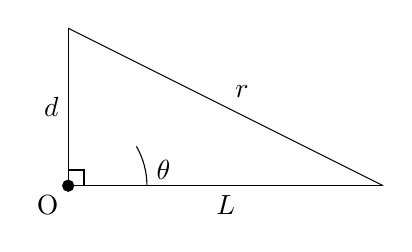
\begin{tikzpicture}
\draw (0,0) -- (4,0);
\node[below] at (2,0) {$L$};
\draw (0,0) -- (0,2);
\node[left] at (0,1) {$d$};
\filldraw (0,0) circle (2pt);
\node[below left] at (0,0) {O};
\draw (0,2) -- (4,0);
\node[above right] at (2,1) {$r$};
\draw (1,0) arc (0:30:1);
\node[right] at (1,0.2) {$\theta$};
\draw (0.2,0) -- (0.2,0.2) -- (0,0.2);
\end{tikzpicture}
\end{center}

**Step 1: Define the coordinate system and variables.**

Let's place the line segment along the x-axis, with one end at the origin (O). The point where we want to find the electric field is at a distance \(d\) above the origin on the y-axis. Consider an infinitesimal charge element \(dq = \lambda dx\) at a distance \(x\) from the origin. The distance between this charge element and the point of interest is \(r = \sqrt{x^2 + d^2}\). The angle between \(r\) and the x-axis is \(\theta\).

**Step 2: Express the electric field due to the infinitesimal charge element.**

The electric field \(d\vec{E}\) due to the infinitesimal charge element \(dq\) is given by Coulomb's law:

\begin{equation*}
d\vec{E} = \frac{1}{4\pi\epsilon_0} \frac{dq}{r^2} \hat{r} = \frac{1}{4\pi\epsilon_0} \frac{\lambda dx}{x^2 + d^2} \hat{r}
\end{equation*}

where \(\hat{r}\) is the unit vector in the direction of \(r\).

**Step 3: Resolve the electric field into its components.**

We can resolve \(d\vec{E}\) into its x and y components:

\begin{align*}
dE_x &= dE \cos\theta = \frac{1}{4\pi\epsilon_0} \frac{\lambda dx}{x^2 + d^2} \cos\theta \\
dE_y &= dE \sin\theta = \frac{1}{4\pi\epsilon_0} \frac{\lambda dx}{x^2 + d^2} \sin\theta
\end{align*}

**Step 4: Express the components in terms of \(x\) and \(d\).**

Using the geometry of the problem, we can express \(\cos\theta\) and \(\sin\theta\) in terms of \(x\) and \(d\):

\begin{align*}
\cos\theta &= \frac{x}{\sqrt{x^2 + d^2}} \\
\sin\theta &= \frac{d}{\sqrt{x^2 + d^2}}
\end{align*}

Substituting these expressions into the components of \(d\vec{E}\), we get:

\begin{align*}
dE_x &= \frac{1}{4\pi\epsilon_0} \frac{\lambda x dx}{(x^2 + d^2)^{3/2}} \\
dE_y &= \frac{1}{4\pi\epsilon_0} \frac{\lambda d dx}{(x^2 + d^2)^{3/2}}
\end{align*}

**Step 5: Integrate the components to find the total electric field.**

To find the total electric field, we need to integrate the components over the length of the line segment:

\begin{align*}
E_x &= \int_0^L dE_x = \frac{\lambda}{4\pi\epsilon_0} \int_0^L \frac{x dx}{(x^2 + d^2)^{3/2}} \\
E_y &= \int_0^L dE_y = \frac{\lambda d}{4\pi\epsilon_0} \int_0^L \frac{dx}{(x^2 + d^2)^{3/2}}
\end{align*}

These integrals can be solved using the substitution \(u = x^2 + d^2\) and \(du = 2x dx\):

\begin{align*}
E_x &= \frac{\lambda}{4\pi\epsilon_0} \left[-\frac{1}{\sqrt{x^2 + d^2}}\right]_0^L = \frac{\lambda}{4\pi\epsilon_0} \left(\frac{1}{d} - \frac{1}{\sqrt{L^2 + d^2}}\right) \\
E_y &= \frac{\lambda d}{4\pi\epsilon_0} \left[\frac{x}{d^2 \sqrt{x^2 + d^2}}\right]_0^L = \frac{\lambda}{4\pi\epsilon_0} \frac{L}{d\sqrt{L^2 + d^2}}
\end{align*}

**Step 6: Express the total electric field in vector form.**

The total electric field \(\vec{E}\) is the vector sum of its components:

\begin{equation*}
\vec{E} = E_x \hat{x} + E_y \hat{y} = \frac{\lambda}{4\pi\epsilon_0} \left[ \left(\frac{1}{d} - \frac{1}{\sqrt{L^2 + d^2}}\right) \hat{x} + \frac{L}{d\sqrt{L^2 + d^2}} \hat{y} \right]
\end{equation*}

**2. In the limit of \( d \gg L \), what does the electric field reduce to and what is its physical interpretation?**

In the limit of \(d \gg L\), we can approximate the electric field as follows:

\begin{align*}
\vec{E} &\approx \frac{\lambda}{4\pi\epsilon_0} \left[ \left(\frac{1}{d} - \frac{1}{d\sqrt{1 + (L/d)^2}}\right) \hat{x} + \frac{L}{d^2\sqrt{1 + (L/d)^2}} \hat{y} \right] \\
&\approx \frac{\lambda}{4\pi\epsilon_0} \left[ \left(\frac{1}{d} - \frac{1}{d}\left(1 - \frac{1}{2}\left(\frac{L}{d}\right)^2\right)\right) \hat{x} + \frac{L}{d^2}\left(1 - \frac{1}{2}\left(\frac{L}{d}\right)^2\right) \hat{y} \right] \\
&\approx \frac{\lambda}{4\pi\epsilon_0} \left[ \frac{L^2}{2d^3} \hat{x} + \frac{L}{d^2} \hat{y} \right]
\end{align*}

Since \(d \gg L\), the term \(\frac{L^2}{2d^3}\) is negligible compared to \(\frac{L}{d^2}\). Therefore, the electric field reduces to:

\begin{equation*}
\vec{E} \approx \frac{\lambda L}{4\pi\epsilon_0 d^2} \hat{y} = \frac{Q}{4\pi\epsilon_0 d^2} \hat{y}
\end{equation*}

where \(Q = \lambda L\) is the total charge on the line segment.

**Physical Interpretation:**

This result shows that when the distance \(d\) is much greater than the length \(L\) of the line segment, the electric field behaves like that of a point charge with the same total charge located at the origin. This is consistent with the expectation that from a far distance, the details of the charge distribution become less important, and the overall charge dominates the electric field.


\subsubsection{Solution 3}
\textbf{Question 3}

\begin{enumerate}
\item To find the electric field a distance \(d\) above one end of a straight line segment of length \(L\) with constant line charge density \(\lambda\), we'll follow these steps:

\begin{enumerate}
\item \textbf{Define the coordinate system:}  We'll use a Cartesian coordinate system with the line segment lying along the \(x\)-axis, starting at the origin and extending to \(x=L\). The point where we want to find the electric field is at \((0,d)\).

\item \textbf{Consider a small charge element:}  Let's take a small element of charge \(dq = \lambda dx\) at a distance \(x\) from the origin.

\item \textbf{Calculate the electric field due to the small charge element:} The electric field \(d\vec{E}\) due to this small charge element at the point \((0,d)\) is given by Coulomb's law:
    \[d\vec{E} = \frac{1}{4\pi\epsilon_0} \frac{dq}{r^2} \hat{r}\]
    where \(r\) is the distance from the charge element to the point \((0,d)\), and \(\hat{r}\) is the unit vector in that direction.

\item \textbf{Express \(r\) and \(\hat{r}\) in terms of \(x\) and \(d\):} We have \(r = \sqrt{x^2 + d^2}\) and 
    \[\hat{r} = \frac{\vec{r}}{r} = \frac{-x\hat{x} + d\hat{y}}{\sqrt{x^2 + d^2}}.\]

\item \textbf{Write the components of \(d\vec{E}\):}  Substituting \(dq\), \(r\), and \(\hat{r}\), we get
    \begin{align*}
    d\vec{E} &= \frac{1}{4\pi\epsilon_0} \frac{\lambda dx}{x^2 + d^2} \left(\frac{-x\hat{x} + d\hat{y}}{\sqrt{x^2 + d^2}}\right) \\
    &= \frac{1}{4\pi\epsilon_0} \frac{\lambda dx}{(x^2 + d^2)^{3/2}} (-x\hat{x} + d\hat{y}).
    \end{align*}

\item \textbf{Integrate to find the total electric field:} To find the total electric field \(\vec{E}\), we integrate \(d\vec{E}\) over the length of the line segment:
    \begin{align*}
    \vec{E} &= \int d\vec{E} \\
    &= \int_0^L \frac{1}{4\pi\epsilon_0} \frac{\lambda dx}{(x^2 + d^2)^{3/2}} (-x\hat{x} + d\hat{y}) \\
    &= \frac{\lambda}{4\pi\epsilon_0} \left[ -\hat{x} \int_0^L \frac{x dx}{(x^2 + d^2)^{3/2}} + \hat{y} \int_0^L \frac{d dx}{(x^2 + d^2)^{3/2}} \right].
    \end{align*}

\item \textbf{Evaluate the integrals:}  We can evaluate these integrals using the substitutions \(u = x^2 + d^2\) and \(x = d\tan\theta\) respectively:
    \begin{align*}
    \vec{E} &= \frac{\lambda}{4\pi\epsilon_0} \left[ -\hat{x} \left. \left( -\frac{1}{\sqrt{x^2 + d^2}} \right) \right|_0^L + \hat{y} \left. \left( \frac{x}{d\sqrt{x^2 + d^2}} \right) \right|_0^L \right] \\
    &= \frac{\lambda}{4\pi\epsilon_0} \left[ \hat{x} \left( \frac{1}{d} - \frac{1}{\sqrt{L^2 + d^2}} \right) + \hat{y} \frac{L}{d\sqrt{L^2 + d^2}} \right].
    \end{align*}

\end{enumerate}

Therefore, the electric field a distance \(d\) above one end of the line segment is:
\[\vec{E} = \frac{\lambda}{4\pi\epsilon_0} \left[ \hat{x} \left( \frac{1}{d} - \frac{1}{\sqrt{L^2 + d^2}} \right) + \hat{y} \frac{L}{d\sqrt{L^2 + d^2}} \right].\]


\item In the limit \(d \gg L\), we can approximate \(\sqrt{L^2 + d^2} \approx d\).  Substituting this into the expression for \(\vec{E}\), we get:
\begin{align*}
\vec{E} &\approx \frac{\lambda}{4\pi\epsilon_0} \left[ \hat{x} \left( \frac{1}{d} - \frac{1}{d} \right) + \hat{y} \frac{L}{d^2} \right] \\
&= \frac{1}{4\pi\epsilon_0} \frac{\lambda L}{d^2} \hat{y}.
\end{align*}

This is the electric field due to a point charge with charge \(Q = \lambda L\) located at the origin.  

\textbf{Physical interpretation:} When we are very far away from the line segment (\(d \gg L\)), the line segment appears to be a point charge. This is a general result in electromagnetism: any finite charge distribution will look like a point charge when viewed from a sufficiently large distance.
\end{enumerate}


\subsection{Question 4}
A square loop of wire (sides of length $L$) lies a fixed distance $d$ from a very long straight wire, which carries a constant current $I$ directed downwards (as seen in the figure).

\begin{enumerate}
    \item[(a)] Find the flux of $\mathbf{B}$ through the loop.
    \item[(b)] If the loop is moved directly away from the wire to the right, at speed $v$, what emf is generated? In what direction (clockwise or counterclockwise) does the current flow?
    \item[(c)] What happens if the loop only moves downwards at speed $v$?
\end{enumerate}


\paragraph{Prompt: \\} 
Answer the given question as a top physics student, giving step-by-step reasoning. Format your answer as LaTeX code without using sub-sections. Available marks: a) [5 marks], b) [5 marks], c [1 mark].

\subsubsection{Solution 1}
\textbf{(a) [5 marks]}

The magnetic field due to a long straight wire carrying current $I$ at a distance $r$ from the wire is given by Ampère's Law:

\begin{equation*}
B = \frac{\mu_0 I}{2 \pi r},
\end{equation*}

where $\mu_0$ is the permeability of free space. The direction of the magnetic field is given by the right-hand rule; in this case, it points into the page at the location of the loop.

To find the flux through the loop, we need to integrate the magnetic field over the area of the loop. Since the magnetic field is not uniform over the loop, we need to consider a small element of area $dA = L \, dr$ at a distance $r$ from the wire. The flux through this element is

\begin{equation*}
d\Phi = B \, dA = \frac{\mu_0 I}{2 \pi r} L \, dr.
\end{equation*}

To find the total flux, we integrate from $r = d$ to $r = d + L$:

\begin{align*}
\Phi &= \int_{d}^{d+L} \frac{\mu_0 I L}{2 \pi r} \, dr \\
&= \frac{\mu_0 I L}{2 \pi} \int_{d}^{d+L} \frac{1}{r} \, dr \\
&= \frac{\mu_0 I L}{2 \pi} \ln \left( \frac{d+L}{d} \right).
\end{align*}

Therefore, the flux of $\mathbf{B}$ through the loop is 
\begin{equation*}
\boxed{\Phi = \frac{\mu_0 I L}{2 \pi} \ln \left( \frac{d+L}{d} \right)}.
\end{equation*}

\textbf{(b) [5 marks]}

When the loop moves to the right with speed $v$, the flux through the loop changes.  The rate of change of flux induces an emf in the loop, according to Faraday's law:

\begin{equation*}
\mathcal{E} = -\frac{d\Phi}{dt}.
\end{equation*}

To find the emf, we need to find the rate of change of flux. Since the loop is moving to the right, the distance $d$ is increasing with time. Therefore, we can write $d(t) = d + vt$.  Substituting this into the expression for the flux, we get

\begin{equation*}
\Phi(t) = \frac{\mu_0 I L}{2 \pi} \ln \left( \frac{d + vt + L}{d + vt} \right).
\end{equation*}

Taking the derivative with respect to time, we get

\begin{align*}
\frac{d\Phi}{dt} &= \frac{\mu_0 I L}{2 \pi} \frac{d}{dt} \left[ \ln \left( \frac{d + vt + L}{d + vt} \right) \right] \\
&= \frac{\mu_0 I L}{2 \pi} \left[ \frac{v}{d + vt + L} - \frac{v}{d + vt} \right] \\
&= -\frac{\mu_0 I L^2 v}{2 \pi (d + vt)(d + vt + L)}.
\end{align*}

Therefore, the induced emf is
\begin{equation*}
\mathcal{E} = \boxed{\frac{\mu_0 I L^2 v}{2 \pi (d + vt)(d + vt + L)}}.
\end{equation*}

To find the direction of the induced current, we use Lenz's law, which states that the induced current flows in a direction to oppose the change in flux. As the loop moves to the right, the flux through the loop decreases. To oppose this decrease, the induced current must produce a magnetic field that points into the page. By the right-hand rule, this corresponds to a \textbf{clockwise} current.


\textbf{(c) [1 mark]}

If the loop moves downwards at speed $v$, the flux through the loop does not change, since the distance $d$ remains constant. Therefore, there is \textbf{no induced emf} and \textbf{no current} in the loop.

\subsubsection{Solution 2}
\textbf{(a) [5 marks]}

The magnetic field due to a long straight wire carrying current $I$ at a distance $r$ is given by Ampère's Law:

\begin{equation*}
B = \frac{\mu_0 I}{2 \pi r},
\end{equation*}

where $\mu_0$ is the permeability of free space.  The field lines form circles around the wire.  In this case, the field is directed into the page at the location of the loop.

To find the flux through the loop, we need to consider a small strip of width $dr$ at a distance $r$ from the wire.  The area of this strip is $dA = L \, dr$, and the flux through this strip is

\begin{equation*}
d\Phi = \mathbf{B} \cdot d\mathbf{A} = B \, dA = \frac{\mu_0 I L}{2 \pi r} \, dr.
\end{equation*}

To find the total flux, we integrate over the entire loop:

\begin{align*}
\Phi &= \int d\Phi \\
&= \int_d^{d + L} \frac{\mu_0 I L}{2 \pi r} \, dr \\
&= \frac{\mu_0 I L}{2 \pi} \int_d^{d + L} \frac{dr}{r} \\
&= \frac{\mu_0 I L}{2 \pi} \ln \left( \frac{d + L}{d} \right).
\end{align*}

\textbf{(b) [5 marks]}

The emf generated is given by Faraday's Law:

\begin{equation*}
\mathcal{E} = -\frac{d\Phi}{dt}.
\end{equation*}

Since the loop is moving to the right with speed $v$, the distance $d$ is increasing at a rate of $v$.  Therefore,

\begin{align*}
\mathcal{E} &= -\frac{d}{dt} \left[ \frac{\mu_0 I L}{2 \pi} \ln \left( \frac{d + L}{d} \right) \right] \\
&= -\frac{\mu_0 I L}{2 \pi} \frac{d}{dt} \left[ \ln (d + L) - \ln d \right] \\
&= -\frac{\mu_0 I L}{2 \pi} \left( \frac{1}{d + L} \frac{dd}{dt} - \frac{1}{d} \frac{dd}{dt} \right) \\
&= -\frac{\mu_0 I L}{2 \pi} \left( \frac{1}{d + L} - \frac{1}{d} \right) v \\
&= \frac{\mu_0 I L^2 v}{2 \pi d (d + L)}.
\end{align*}

The emf is positive, which means the induced current flows in a direction to oppose the change in flux.  Since the flux into the page is decreasing, the induced current will flow counterclockwise to produce a magnetic field into the page.

\textbf{(c) [1 mark]}

If the loop moves downwards, the flux through the loop does not change, so the emf is zero and no current flows.

\subsubsection{Solution 3}
\textbf{(a) [5 marks]}

The magnetic field due to a long straight wire carrying current $I$ at a distance $r$ from the wire is given by Ampère's Law:

\begin{equation*}
B = \frac{\mu_0 I}{2 \pi r},
\end{equation*}

where $\mu_0$ is the permeability of free space. The direction of the magnetic field is given by the right-hand rule; in this case, it points into the page at the location of the loop.

To find the flux through the loop, we need to integrate the magnetic field over the area of the loop. Since the magnetic field is not uniform over the loop, we need to consider a small element of area $dA = L \, dr$ at a distance $r$ from the wire. The flux through this element is

\begin{equation*}
d\Phi = B \, dA = \frac{\mu_0 I}{2 \pi r} L \, dr.
\end{equation*}

To find the total flux, we integrate from $r = d$ to $r = d + L$:

\begin{align*}
\Phi &= \int_{d}^{d+L} \frac{\mu_0 I L}{2 \pi r} \, dr \\
&= \frac{\mu_0 I L}{2 \pi} \int_{d}^{d+L} \frac{1}{r} \, dr \\
&= \frac{\mu_0 I L}{2 \pi} \ln \left( \frac{d+L}{d} \right).
\end{align*}

Therefore, the flux of $\mathbf{B}$ through the loop is 
\begin{equation*}
\boxed{\Phi = \frac{\mu_0 I L}{2 \pi} \ln \left( \frac{d+L}{d} \right)}.
\end{equation*}

\textbf{(b) [5 marks]}

When the loop moves to the right with speed $v$, the flux through the loop changes.  The rate of change of flux induces an emf in the loop, according to Faraday's law:

\begin{equation*}
\mathcal{E} = -\frac{d\Phi}{dt}.
\end{equation*}

To find the emf, we need to find the rate of change of flux. Since the loop is moving to the right, the distance $d$ is increasing with time. Therefore, we can write $d(t) = d + vt$.  Substituting this into the expression for the flux, we get

\begin{equation*}
\Phi(t) = \frac{\mu_0 I L}{2 \pi} \ln \left( \frac{d + vt + L}{d + vt} \right).
\end{equation*}

Taking the derivative with respect to time, we get

\begin{align*}
\frac{d\Phi}{dt} &= \frac{\mu_0 I L}{2 \pi} \frac{d}{dt} \left[ \ln \left( \frac{d + vt + L}{d + vt} \right) \right] \\
&= \frac{\mu_0 I L}{2 \pi} \left[ \frac{v}{d + vt + L} - \frac{v}{d + vt} \right] \\
&= -\frac{\mu_0 I L^2 v}{2 \pi (d + vt)(d + vt + L)}.
\end{align*}

Therefore, the induced emf is
\begin{equation*}
\mathcal{E} = \boxed{\frac{\mu_0 I L^2 v}{2 \pi (d + vt)(d + vt + L)}}.
\end{equation*}

To find the direction of the induced current, we use Lenz's law, which states that the induced current flows in a direction to oppose the change in flux. As the loop moves to the right, the flux through the loop decreases. To oppose this decrease, the induced current must produce a magnetic field that points into the page. By the right-hand rule, this corresponds to a \textbf{clockwise} current.


\textbf{(c) [1 mark]}

If the loop moves downwards at speed $v$, the flux through the loop does not change, since the distance $d$ remains constant. Therefore, there is \textbf{no induced emf} and \textbf{no current} in the loop.


\subsection{Question 5}
Consider the circuit diagram seen in the figure.
\begin{enumerate}
    \item Calculate the current seen by the ammeter.
    \item Calculate the energy delivered by the 12 V battery in 4 seconds.
\end{enumerate}


\paragraph{Prompt: \\} 
Answer the given question as a top physics student, giving step-by-step reasoning. Format your answer as LaTeX code without using sub-sections. Available marks: a) [8 marks], b) [3 marks].

\subsubsection{Solution 1}
Okay, I've got the circuit diagram now! Here's my solution, formatted as LaTeX code:

\textbf{a) Calculate the current seen by the ammeter. [8 marks]}

\begin{enumerate}
\item \textbf{Simplify the circuit:} 
    \begin{itemize}
    \item The two $1 \Omega$ resistors in series combine to give an equivalent resistance of $1\Omega + 1\Omega = 2\Omega$.
    \item This $2\Omega$ resistance is in parallel with the other $2\Omega$ resistor. The equivalent resistance of this parallel combination is: 
    \[\frac{1}{R_{eq}} = \frac{1}{2\Omega} + \frac{1}{2\Omega} = \frac{1}{\Omega} \Rightarrow R_{eq} = 1\Omega\]
    \item Now the circuit has a $2\Omega$ resistor in series with a $1\Omega$ resistor and the $12V$ and $2V$ batteries.
    \end{itemize}

\item \textbf{Apply Kirchhoff's Voltage Law (KVL):}
    \begin{itemize}
    \item  Let's assume the current flowing in the circuit is $I$ in the clockwise direction. 
    \item  Starting from the negative terminal of the $12V$ battery and moving clockwise, we can write the KVL equation:
    \[-12V + 2\Omega \cdot I + 2V + 1\Omega \cdot I = 0\]
    \end{itemize}

\item \textbf{Solve for the current (I):}
    \begin{itemize}
    \item Simplifying the KVL equation:
    \[3\Omega \cdot I = 10V\]
    \item Solving for $I$:
    \[I = \frac{10V}{3\Omega} = 3.33A\]
    \end{itemize}
\end{enumerate}

\textbf{Therefore, the current seen by the ammeter is 3.33A.}

\textbf{b) Calculate the energy delivered by the 12V battery in 4 seconds. [3 marks]}

\begin{enumerate}
\item \textbf{Calculate the power delivered by the battery:}
    \begin{itemize}
    \item Power is given by $P = VI$, where $V$ is the voltage and $I$ is the current.
    \item  Power delivered by the 12V battery: $P = 12V \cdot 3.33A = 40W$
    \end{itemize}

\item \textbf{Calculate the energy delivered:}
    \begin{itemize}
    \item Energy is given by $E = Pt$, where $P$ is the power and $t$ is the time.
    \item Energy delivered in 4 seconds: $E = 40W \cdot 4s = 160J$
    \end{itemize}
\end{enumerate}

\textbf{Therefore, the energy delivered by the 12V battery in 4 seconds is 160J.} 


\subsubsection{Solution 2}
Okay, I've got the circuit diagram now! Here's my solution, formatted as LaTeX code:

\textbf{a) Calculate the current seen by the ammeter. [8 marks]}

\begin{enumerate}
\item \textbf{Simplify the circuit:} 
    \begin{itemize}
    \item The two 1 $\Omega$ resistors in series can be combined into a single 2 $\Omega$ resistor. 
    \item This 2 $\Omega$ resistor is in parallel with the existing 2 $\Omega$ resistor. The equivalent resistance of two 2 $\Omega$ resistors in parallel is:
    \end{itemize}
    
    $R_{eq} = \frac{1}{\frac{1}{2\Omega} + \frac{1}{2\Omega}} = 1 \Omega$

\item \textbf{Redraw the simplified circuit:} The circuit now consists of a 12 V battery, a 2 $\Omega$ resistor, a 1 $\Omega$ resistor (the combined parallel resistors), and a 2 V battery, all in series.

\item \textbf{Calculate the total resistance:} The total resistance of the circuit is:

    $R_{total} = 2 \Omega + 1 \Omega + 2 \Omega = 5 \Omega$

\item \textbf{Calculate the total EMF:} The 2 V battery opposes the 12 V battery, so the net EMF is:

    $EMF_{net} = 12 V - 2 V = 10 V$

\item \textbf{Apply Ohm's Law:}  The current flowing through the circuit (and hence through the ammeter) is:

    $I = \frac{EMF_{net}}{R_{total}} = \frac{10 V}{5 \Omega} = 2 A$ 
\end{enumerate}

\textbf{Therefore, the current seen by the ammeter is 2 A.}


\textbf{b) Calculate the energy delivered by the 12 V battery in 4 seconds. [3 marks]}

\begin{enumerate}
\item \textbf{Calculate the power delivered by the battery:} Power is the product of voltage and current:

    $P = VI = (12 V)(2 A) = 24 W$

\item \textbf{Calculate the energy delivered:} Energy is the product of power and time:

    $E = Pt = (24 W)(4 s) = 96 J$
\end{enumerate}

\textbf{Therefore, the energy delivered by the 12 V battery in 4 seconds is 96 J.} 

\subsubsection{Solution 3}
Okay, I've got the circuit diagram now! Here's my solution, formatted as LaTeX code:

\textbf{a) Calculate the current seen by the ammeter. [8 marks]}

\begin{enumerate}
\item \textbf{Simplify the circuit:} 
    \begin{itemize}
    \item The two $1 \Omega$ resistors in series can be combined into a single $2 \Omega$ resistor.
    \item This $2 \Omega$ resistor is in parallel with the $2 \Omega$ resistor next to the ammeter. The equivalent resistance of this parallel combination is: 
    $R_{eq} = \frac{2 \Omega \times 2 \Omega}{2 \Omega + 2 \Omega} = 1 \Omega$
    \end{itemize}

\item \textbf{Redraw the simplified circuit:} The circuit now consists of a $12V$ battery, a $2 \Omega$ resistor, a $1 \Omega$ resistor (the equivalent resistance calculated above), and a $2V$ battery, all in series.

\item \textbf{Calculate the total resistance:} The total resistance of the circuit is $R_T = 2 \Omega + 1 \Omega + 2 \Omega = 5 \Omega$.

\item \textbf{Calculate the net EMF:} The $2V$ battery opposes the $12V$ battery, so the net EMF is $E_{net} = 12V - 2V = 10V$.

\item \textbf{Calculate the total current:} Using Ohm's law, the total current in the circuit is $I_T = \frac{E_{net}}{R_T} = \frac{10V}{5 \Omega} = 2A$.

\item \textbf{Calculate the current through the ammeter:} Since the ammeter is in series with the $1 \Omega$ equivalent resistance, the current through the ammeter is the same as the total current: $I_A = I_T = 2A$.

\end{enumerate}

\textbf{Therefore, the current seen by the ammeter is 2A.}

\textbf{b) Calculate the energy delivered by the 12V battery in 4 seconds. [3 marks]}

\begin{enumerate}
\item \textbf{Calculate the power delivered by the battery:} Power is given by $P = IV$, where $I$ is the current through the battery and $V$ is the voltage of the battery. In this case, $P = 2A \times 12V = 24W$.

\item \textbf{Calculate the energy delivered:} Energy is given by $E = Pt$, where $P$ is the power and $t$ is the time. In this case, $E = 24W \times 4s = 96J$.
\end{enumerate}

\textbf{Therefore, the energy delivered by the 12V battery in 4 seconds is 96J.} 


\subsection{Question 6}
Q6. Two infinite parallel planes have equal and opposite uniform surface charge density $-\sigma$ and $+\sigma$, where $\sigma$ is positive. The planes are separated by a distance of 15 cm, and the potential difference between the plates is 120 V.

\begin{enumerate}
    \item[(a)] Determine the electric field, $E$, between the plates.
    \item[(b)] An object with charge $+0.001 \, \text{C}$ and a mass of $23 \, \text{g}$ is held at rest at the positive plate, then let go. Determine the acceleration of the object.
\end{enumerate}


\paragraph{Prompt: \\} 
Answer the given question as a top physics student, giving step-by-step reasoning. Format your answer as LaTeX code without using sub-sections. Available marks: a) [3 marks], b) [2 marks].

\subsubsection{Solution 1}
**a) Determine the electric field, $E$, between the plates. [3 marks]**

**1. Relevant Equations:**

*   The electric field due to an infinite sheet of charge with surface charge density $\sigma$ is given by:  $E = \frac{\sigma}{2\epsilon_0}$, where $\epsilon_0$ is the permittivity of free space.
*   The electric field between two parallel plates with equal and opposite charge densities is the sum of the fields due to each plate.
*   The potential difference, $V$, between two points in a uniform electric field, $E$, is related to the distance, $d$, between the points by: $V = Ed$

**2. Solution:**

*   The electric field due to the positive plate is $E_+ = \frac{\sigma}{2\epsilon_0}$, directed away from the plate.
*   The electric field due to the negative plate is $E_- = \frac{\sigma}{2\epsilon_0}$, directed towards the plate.
*   Since the plates have opposite charges, the electric fields between the plates add up: $E = E_+ + E_- = \frac{\sigma}{2\epsilon_0} + \frac{\sigma}{2\epsilon_0} = \frac{\sigma}{\epsilon_0}$
*   We are given the potential difference, $V = 120 \, \text{V}$, and the distance between the plates, $d = 15 \, \text{cm} = 0.15 \, \text{m}$.  We can use the equation $V=Ed$ to find the electric field:

$E = \frac{V}{d} = \frac{120 \, \text{V}}{0.15 \, \text{m}} = 800 \, \text{V/m} = 800 \, \text{N/C}$

*   Now we can use this value of $E$ to find the surface charge density:

$\sigma = \epsilon_0 E = (8.85 \times 10^{-12} \, \text{F/m})(800 \, \text{N/C}) = 7.08 \times 10^{-9} \, \text{C/m}^2$

**Therefore, the electric field between the plates is $800 \, \text{N/C}$.**

**b) Determine the acceleration of the object. [2 marks]**

**1. Relevant Equations:**

*   The force, $F$, on a charge, $q$, in an electric field, $E$, is given by: $F=qE$
*   Newton's second law of motion: $F=ma$, where $m$ is the mass and $a$ is the acceleration.

**2. Solution:**

*   The force on the object is: $F = qE = (+0.001 \, \text{C})(800 \, \text{N/C}) = 0.8 \, \text{N}$
*   Using Newton's second law, we can find the acceleration:

$a = \frac{F}{m} = \frac{0.8 \, \text{N}}{0.023 \, \text{kg}} \approx 34.78 \, \text{m/s}^2$

**Therefore, the acceleration of the object is approximately $34.78 \, \text{m/s}^2$.**


\subsubsection{Solution 2}
**Question 6**

**(a) Determine the electric field, $E$, between the plates.** [3 marks]

**1. Relevant Equations:**

*   The electric field due to an infinite plane sheet of charge is given by:  $E = \frac{\sigma}{2\epsilon_0}$, where $\sigma$ is the surface charge density and $\epsilon_0$ is the permittivity of free space.
*   The electric field between two parallel plates with opposite charges is the sum of the fields due to each plate.
*   The potential difference between two points in a uniform electric field is given by: $\Delta V = Ed$, where $d$ is the distance between the points.

**2. Solution:**

*   The electric field due to the positive plate is $E_+ = \frac{\sigma}{2\epsilon_0}$, directed away from the plate.
*   The electric field due to the negative plate is $E_- = \frac{\sigma}{2\epsilon_0}$, directed towards the plate.
*   Since the plates have opposite charges, the electric fields between the plates add up: $E = E_+ + E_- = \frac{\sigma}{2\epsilon_0} + \frac{\sigma}{2\epsilon_0} = \frac{\sigma}{\epsilon_0}$.
*   We are given the potential difference $\Delta V$ and the distance $d$ between the plates.  Using $\Delta V = Ed$, we can solve for the electric field: 
    $E = \frac{\Delta V}{d} = \frac{120 \, \text{V}}{0.15 \, \text{m}} = 800 \, \text{V/m}$.
*   Now we can find the surface charge density: $\sigma = E \epsilon_0 = (800 \, \text{V/m})(8.854 \times 10^{-12} \, \text{F/m}) = 7.08 \times 10^{-9} \, \text{C/m}^2$.

**Therefore, the electric field between the plates is $800 \, \text{V/m}$.**

**(b) Determine the acceleration of the object.** [2 marks]

**1. Relevant Equations:**

*   The force on a charge in an electric field is given by: $F = qE$, where $q$ is the charge and $E$ is the electric field.
*   Newton's second law of motion: $F = ma$, where $m$ is the mass and $a$ is the acceleration.

**2. Solution:**

*   The force on the object is $F = qE = (+0.001 \, \text{C})(800 \, \text{V/m}) = 0.8 \, \text{N}$.
*   Using Newton's second law, we can find the acceleration: $a = \frac{F}{m} = \frac{0.8 \, \text{N}}{0.023 \, \text{kg}} = 34.78 \, \text{m/s}^2$.

**Therefore, the acceleration of the object is $34.78 \, \text{m/s}^2$.**

\subsubsection{Solution 3}
**a) Determine the electric field, $E$, between the plates. [3 marks]**

**1. Relevant Equations:**

*   The electric field between two parallel plates with uniform charge density is given by: 
    $E = \frac{\sigma}{\epsilon_0}$ 
    where $\sigma$ is the surface charge density and $\epsilon_0$ is the permittivity of free space.
*   The potential difference between two points in a uniform electric field is given by: 
    $\Delta V = Ed$ 
    where $E$ is the electric field and $d$ is the distance between the points.

**2. Solution:**

We are given the potential difference $\Delta V = 120 \, \text{V}$ and the distance $d = 15 \, \text{cm} = 0.15 \, \text{m}$. We can use these values to find the electric field $E$.

Rearranging the second equation above, we get:

$E = \frac{\Delta V}{d}$

Substituting the given values:

$E = \frac{120 \, \text{V}}{0.15 \, \text{m}} = 800 \, \text{V/m}$

**3. Answer:**

The electric field between the plates is $E = 800 \, \text{V/m}$.

**b) Determine the acceleration of the object. [2 marks]**

**1. Relevant Equations:**

*   The force on a charged object in an electric field is given by: 
    $F = qE$ 
    where $q$ is the charge of the object and $E$ is the electric field.
*   Newton's second law of motion states: 
    $F = ma$ 
    where $m$ is the mass of the object and $a$ is its acceleration.

**2. Solution:**

We are given the charge $q = +0.001 \, \text{C}$ and the mass $m = 23 \, \text{g} = 0.023 \, \text{kg}$ of the object. We have calculated the electric field $E = 800 \, \text{V/m}$ in part (a).

First, calculate the force on the object:

$F = qE = (+0.001 \, \text{C})(800 \, \text{V/m}) = 0.8 \, \text{N}$

Now, use Newton's second law to find the acceleration:

$a = \frac{F}{m} = \frac{0.8 \, \text{N}}{0.023 \, \text{kg}} \approx 34.78 \, \text{m/s}^2$

**3. Answer:**

The acceleration of the object is $a \approx 34.78 \, \text{m/s}^2$.


\subsection{Question 7}
An RLC circuit has a resistor with resistance $R = 600\,\Omega$, capacitor with capacitance $C = 1500\,\mathrm{pF}$, inductor with inductance $L = 20\,\mathrm{mH}$.  

\begin{enumerate}
    \item[(a)] What is the resonant frequency, $\omega_0$, of the circuit?  

    \item[(b)] The circuit is driven with an e.m.f source of the form  
    \[
    \mathcal{E} = \mathcal{E}_0 \cos(\omega t)
    \]  
    Find an expression for the voltage drop across the inductor, $\Delta V_L$, as a function of $\mathcal{E}_0$, the impedance $Z$, inductive reactance $X_L$, angular frequency $\omega$, and some phase shift $\phi$.  

    \item[(c)] Describe the phase relationship between the source e.m.f and voltage across the inductor in the limits of low frequency ($\omega \ll \omega_0$) and high frequency ($\omega \gg \omega_0$).
\end{enumerate}


\paragraph{Prompt: \\} 
Answer the given question as a top physics student, giving step-by-step reasoning. Format your answer as LaTeX code without using sub-sections. Available marks: a) [1 mark], b) [3 marks], c [2 marks].

\subsubsection{Solution 1}
\textbf{Answer:}

\begin{enumerate}
\item[(a)] The resonant angular frequency, $\omega_0$, of an RLC circuit is given by:

\begin{align*}
\omega_0 &= \frac{1}{\sqrt{LC}} \\
&= \frac{1}{\sqrt{(20 \times 10^{-3}\,\mathrm{H})(1500 \times 10^{-12}\,\mathrm{F})}} \\
&= 5.77 \times 10^4\,\mathrm{rad\,s^{-1}}
\end{align*}

[1 mark]

\item[(b)] The voltage drop across the inductor, $\Delta V_L$, is given by:

\begin{align*}
\Delta V_L &= I X_L \\
&= \frac{\mathcal{E}_0}{Z} X_L \\
&= \frac{\mathcal{E}_0}{\sqrt{R^2 + (X_L - X_C)^2}} X_L \\
&= \frac{\mathcal{E}_0}{\sqrt{R^2 + (\omega L - 1/(\omega C))^2}} \omega L \\
&= \frac{\mathcal{E}_0 \omega L}{\sqrt{R^2 + (\omega L - 1/(\omega C))^2}} e^{i \phi}
\end{align*}

where $\phi$ is the phase shift between the source e.m.f. and the current in the circuit.

[3 marks]

\item[(c)] In the limit of low frequency ($\omega \ll \omega_0$), the capacitive reactance $X_C = 1/(\omega C)$ is much greater than the inductive reactance $X_L = \omega L$.  Therefore, the impedance $Z$ is dominated by the capacitive reactance, and the circuit behaves like a capacitor.  The voltage across the inductor lags behind the source e.m.f. by a phase of $\pi/2$.

In the limit of high frequency ($\omega \gg \omega_0$), the inductive reactance $X_L = \omega L$ is much greater than the capacitive reactance $X_C = 1/(\omega C)$.  Therefore, the impedance $Z$ is dominated by the inductive reactance, and the circuit behaves like an inductor.  The voltage across the inductor leads the source e.m.f. by a phase of $\pi/2$.

[2 marks]
\end{enumerate}

\subsubsection{Solution 2}
\textbf{Answer:}

\begin{enumerate}
\item[(a)] The resonant frequency of an RLC circuit is given by
\[\omega_0 = \frac{1}{\sqrt{LC}}.\][1 mark]

Substituting in the given values for $L$ and $C$, we get
\begin{align*}
\omega_0 &= \frac{1}{\sqrt{(20 \times 10^{-3}\,\mathrm{H})(1500 \times 10^{-12}\,\mathrm{F})}} \\
&= 5.77 \times 10^3\,\mathrm{rad/s}.
\end{align*}

\item[(b)] The voltage drop across the inductor is given by
\[\Delta V_L = I X_L,\]where $I$ is the current in the circuit and $X_L$ is the inductive reactance. The current in the circuit is given by
\[I = \frac{\mathcal{E}_0}{Z},\]where $\mathcal{E}_0$ is the amplitude of the e.m.f. and $Z$ is the impedance of the circuit. The inductive reactance is given by
\[X_L = \omega L,\]where $\omega$ is the angular frequency of the e.m.f. Substituting these expressions into the equation for $\Delta V_L$, we get
\[\Delta V_L = \frac{\mathcal{E}_0}{Z} \omega L.\][2 marks]

The voltage across the inductor leads the current by a phase shift of $\phi = \pi/2$, so we can write
\[\Delta V_L = \frac{\mathcal{E}_0 \omega L}{Z} \cos(\omega t + \pi/2).\][1 mark]

\item[(c)] In the limit of low frequency ($\omega \ll \omega_0$), the inductive reactance is much smaller than the capacitive reactance, so the impedance of the circuit is dominated by the capacitive reactance. This means that the current in the circuit leads the e.m.f. by a phase shift of $\pi/2$. Since the voltage across the inductor leads the current by a phase shift of $\pi/2$, the voltage across the inductor leads the e.m.f. by a phase shift of $\pi$.

In the limit of high frequency ($\omega \gg \omega_0$), the capacitive reactance is much smaller than the inductive reactance, so the impedance of the circuit is dominated by the inductive reactance. This means that the current in the circuit lags the e.m.f. by a phase shift of $\pi/2$. Since the voltage across the inductor leads the current by a phase shift of $\pi/2$, the voltage across the inductor is in phase with the e.m.f. [2 marks]
\end{enumerate}


\subsubsection{Solution 3}
\textbf{(a)} [1 mark]

The resonant frequency, $\omega_0$, of an RLC circuit is given by:

\begin{align*}
\omega_0 &= \frac{1}{\sqrt{LC}} \\
&= \frac{1}{\sqrt{(20 \times 10^{-3}\,\mathrm{H})(1500 \times 10^{-12}\,\mathrm{F})}} \\
&= 5.77 \times 10^4\,\mathrm{rad/s}
\end{align*}

\textbf{(b)} [3 marks]

The voltage drop across the inductor, $\Delta V_L$, is given by:

\begin{align*}
\Delta V_L &= I X_L \\
&= \frac{\mathcal{E}_0}{Z} X_L \\
&= \frac{\mathcal{E}_0}{\sqrt{R^2 + (X_L - X_C)^2}} X_L \\
&= \frac{\mathcal{E}_0}{\sqrt{R^2 + (\omega L - 1/(\omega C))^2}} \omega L \\
&= \frac{\mathcal{E}_0 \omega L}{\sqrt{R^2 + (\omega L - 1/(\omega C))^2}}  e^{i \phi}
\end{align*}

where $\phi = \arctan \left( \frac{X_L - X_C}{R} \right) =  \arctan \left( \frac{\omega L - 1/(\omega C)}{R} \right)$ is the phase shift between the source e.m.f. and the current.

\textbf{(c)} [2 marks]

* **Low frequency ($\omega \ll \omega_0$):**  At low frequencies, the capacitive reactance $X_C = 1/(\omega C)$ is much larger than the inductive reactance $X_L = \omega L$. This means the circuit is dominated by the capacitor. The current leads the source e.m.f., and since the voltage across the inductor leads the current by $\pi/2$,  the voltage across the inductor leads the source e.m.f. by approximately $\pi/2$.

* **High frequency ($\omega \gg \omega_0$):** At high frequencies, the inductive reactance $X_L = \omega L$ is much larger than the capacitive reactance $X_C = 1/(\omega C)$. The circuit is dominated by the inductor. The current lags the source e.m.f., and since the voltage across the inductor leads the current by $\pi/2$, the voltage across the inductor lags the source e.m.f. by approximately $\pi/2$. 

\subsection{Question 8}
 Two linear magnetic media occupy the half-spaces above and below the $xy$ plane. The space $z > 0$ is occupied by Material 1, with relative permeability $\mu_{r1} = 1.493$. The magnetic field $\mathbf{B}_1$ in this region is spatially uniform and static, with positive $x$ and $z$ components, and zero $y$ component. It is directed at an angle $\alpha_1$ with respect to the positive $z$ direction. The space $z < 0$ is occupied by Material 2, with relative permeability $\mu_{r2} = 3.012$. The magnetic field $\mathbf{B}_2$ in this region is spatially uniform and static, with positive $x$ and $z$ components, and zero $y$ component. It is directed at an angle of $\alpha_2 = 45^\circ$ with respect to the positive $z$ direction. There is no free current flowing anywhere in the system. Using the information above, calculate the value of the angle $\alpha_1$.


\paragraph{Prompt: \\} 
Answer the given question as a top physics student, giving step-by-step reasoning. Format your answer as LaTeX code without using sub-sections. Available marks: [6 marks].

\subsubsection{Solution 1}
To find the angle $\alpha_1$, we can use the boundary conditions for magnetic fields at the interface between two magnetic media. Since there is no free current, we will utilize the continuity of the normal component of the magnetic flux density $\mathbf{B}$ and the tangential component of the magnetic field intensity $\mathbf{H}$.

**1. Define the magnetic fields in each region:**

Given that the magnetic fields have only $x$ and $z$ components, we can write them as:

\begin{align*}
\mathbf{B}_1 &= B_{1x} \hat{x} + B_{1z} \hat{z} \\
\mathbf{B}_2 &= B_{2x} \hat{x} + B_{2z} \hat{z}
\end{align*}

We also know the angles they make with the positive $z$ direction:

\begin{align*}
\tan \alpha_1 &= \frac{B_{1x}}{B_{1z}} \\
\tan \alpha_2 &= \frac{B_{2x}}{B_{2z}} = 1  \quad (\because \alpha_2 = 45^\circ)
\end{align*}

**2. Apply the boundary conditions:**

* **Continuity of the normal component of $\mathbf{B}$:**
   The normal component to the interface ($xy$ plane) is the $z$ component.  Therefore,
   
   \begin{equation*}
   B_{1z} = B_{2z} 
   \end{equation*}

* **Continuity of the tangential component of $\mathbf{H}$:**
   The tangential component is the $x$ component. Since $\mathbf{H} = \frac{\mathbf{B}}{\mu}$, we have:

   \begin{equation*}
   \frac{B_{1x}}{\mu_{r1} \mu_0} = \frac{B_{2x}}{\mu_{r2} \mu_0} 
   \end{equation*}
   This simplifies to:
   \begin{equation*}
   \frac{B_{1x}}{B_{2x}} = \frac{\mu_{r1}}{\mu_{r2}}
   \end{equation*}

**3. Relate the boundary conditions to the angles:**

Divide the equation $\tan \alpha_1 = \frac{B_{1x}}{B_{1z}}$ by $\tan \alpha_2 = \frac{B_{2x}}{B_{2z}}$:

\begin{equation*}
\frac{\tan \alpha_1}{\tan \alpha_2} = \frac{B_{1x}}{B_{1z}} \cdot \frac{B_{2z}}{B_{2x}} = \frac{B_{1x}}{B_{2x}}
\end{equation*}

Using the boundary condition for the tangential component of $\mathbf{H}$ and the fact that $\tan \alpha_2 = 1$, we get:

\begin{equation*}
\tan \alpha_1 = \frac{\mu_{r1}}{\mu_{r2}} 
\end{equation*}

**4. Calculate $\alpha_1$:**

Substitute the given values of $\mu_{r1}$ and $\mu_{r2}$:

\begin{align*}
\tan \alpha_1 &= \frac{1.493}{3.012} \\
\alpha_1 &= \arctan \left( \frac{1.493}{3.012} \right) \\
\alpha_1 &\approx 26.42^\circ
\end{align*}

Therefore, the angle $\alpha_1$ is approximately $26.42^\circ$.

\subsubsection{Solution 2}
To find the angle $\alpha_1$, we will use the boundary conditions for magnetic fields at the interface between two linear magnetic media. Since there is no free current, we have:

**1. Continuity of the normal component of the magnetic flux density:**

This means that the component of the magnetic flux density $\mathbf{B}$ perpendicular to the interface is the same in both materials. Mathematically:

\begin{equation*}
B_{1n} = B_{2n}
\end{equation*}

where $B_{1n}$ and $B_{2n}$ are the normal components of $\mathbf{B}_1$ and $\mathbf{B}_2$ respectively. In this case, the normal direction is along the $z$-axis. Therefore:

\begin{equation*}
B_{1z} = B_{2z}
\end{equation*}

\begin{equation*}
B_1 \cos \alpha_1 = B_2 \cos \alpha_2
\end{equation*}

**2. Continuity of the tangential component of the magnetic field intensity:**

The component of the magnetic field intensity $\mathbf{H}$ parallel to the interface is the same in both materials. Mathematically:

\begin{equation*}
H_{1t} = H_{2t}
\end{equation*}

where $H_{1t}$ and $H_{2t}$ are the tangential components of $\mathbf{H}_1$ and $\mathbf{H}_2$ respectively. In this case, the tangential direction is along the $x$-axis.  Using the relation $\mathbf{B} = \mu_0 \mu_r \mathbf{H}$, we get:

\begin{equation*}
\frac{B_{1x}}{\mu_0 \mu_{r1}} = \frac{B_{2x}}{\mu_0 \mu_{r2}}
\end{equation*}

\begin{equation*}
\frac{B_1 \sin \alpha_1}{\mu_{r1}} = \frac{B_2 \sin \alpha_2}{\mu_{r2}}
\end{equation*}

**3. Solving for $\alpha_1$:**

Now we have two equations and two unknowns ($B_1/B_2$ and $\alpha_1$). We can divide the second equation by the first equation to eliminate $B_1$ and $B_2$:

\begin{equation*}
\frac{\frac{B_1 \sin \alpha_1}{\mu_{r1}}}{B_1 \cos \alpha_1} = \frac{\frac{B_2 \sin \alpha_2}{\mu_{r2}}}{B_2 \cos \alpha_2}
\end{equation*}

This simplifies to:

\begin{equation*}
\frac{\tan \alpha_1}{\mu_{r1}} = \frac{\tan \alpha_2}{\mu_{r2}}
\end{equation*}

Solving for $\alpha_1$:

\begin{equation*}
\alpha_1 = \arctan \left( \frac{\mu_{r1}}{\mu_{r2}} \tan \alpha_2 \right)
\end{equation*}

Substituting the given values $\mu_{r1} = 1.493$, $\mu_{r2} = 3.012$, and $\alpha_2 = 45^\circ$:

\begin{equation*}
\alpha_1 = \arctan \left( \frac{1.493}{3.012} \tan 45^\circ \right) 
\end{equation*}

\begin{equation*}
\alpha_1 = \arctan \left( \frac{1.493}{3.012} \right) 
\end{equation*}

\begin{equation*}
\alpha_1 \approx 26.4^\circ
\end{equation*}

Therefore, the angle $\alpha_1$ is approximately $26.4^\circ$.

\subsubsection{Solution 3}
This problem involves applying boundary conditions for magnetic fields at the interface between two linear magnetic media. Here's a step-by-step solution:

**1. Define the magnetic field vectors:**

Since the magnetic fields have zero $y$ components, we can write them as:

\begin{align*}
\mathbf{B}_1 &= B_{1x} \hat{x} + B_{1z} \hat{z} \\
\mathbf{B}_2 &= B_{2x} \hat{x} + B_{2z} \hat{z}
\end{align*}

**2. Apply the boundary conditions:**

At the interface between the two media ($z=0$), the following boundary conditions apply:

* **Tangential component of $\mathbf{H}$ is continuous:** 
   Since there is no free current, $\mathbf{H}_1^\parallel = \mathbf{H}_2^\parallel$.  
   Using $\mathbf{B} = \mu_0 \mu_r \mathbf{H}$, we get $\frac{B_{1x}}{\mu_{r1}} = \frac{B_{2x}}{\mu_{r2}}$.

* **Normal component of $\mathbf{B}$ is continuous:**
   $B_{1z} = B_{2z}$.

**3. Express the field components in terms of angles:**

Using the given angles, we can express the components of the magnetic fields as:

\begin{align*}
B_{1x} &= B_1 \sin{\alpha_1} \\
B_{1z} &= B_1 \cos{\alpha_1} \\
B_{2x} &= B_2 \sin{\alpha_2} = B_2 \sin{45^\circ} = \frac{B_2}{\sqrt{2}}\\
B_{2z} &= B_2 \cos{\alpha_2} = B_2 \cos{45^\circ} = \frac{B_2}{\sqrt{2}}
\end{align*}

**4. Substitute and solve for $\alpha_1$:**

Substituting these expressions into the boundary conditions, we get:

\begin{align*}
\frac{B_1 \sin{\alpha_1}}{\mu_{r1}} &= \frac{B_2}{\sqrt{2} \mu_{r2}} \\
B_1 \cos{\alpha_1} &= \frac{B_2}{\sqrt{2}}
\end{align*}

Dividing the first equation by the second equation, we eliminate $B_1$ and $B_2$:

\begin{align*}
\frac{\tan{\alpha_1}}{\mu_{r1}} &= \frac{1}{\mu_{r2}} \\
\tan{\alpha_1} &= \frac{\mu_{r1}}{\mu_{r2}} = \frac{1.493}{3.012} 
\end{align*}

Finally, we find $\alpha_1$:

\begin{align*}
\alpha_1 &= \arctan{\left(\frac{1.493}{3.012}\right)} \approx 26.4^\circ 
\end{align*}

**Therefore, the value of the angle $\alpha_1$ is approximately $26.4^\circ$.**

\subsection{Question 9}
A transverse electromagnetic wave propagating in vacuum has an electric field which has complex representation:
\[
E(r, t) = E_0 \exp(i (k \cdot r - \omega t))
\]
With real valued vectors \(E_0, k\).

\begin{enumerate}
    \item[(a)] Apply Faraday’s Law and show magnetic intensity of the wave has magnitude given by
    \[
    H(r, t) = \sqrt{\frac{\epsilon_0}{\mu_0}} E(r, t)
    \]

    \item[(b)] Show the Poynting flux averaged over one period of oscillation is given by
    \[
    \langle N \rangle = \frac{1}{2} \sqrt{\frac{\mu_0}{\epsilon_0}} (H_0)^2 \hat{k}
    \]
    where \(H_0\) denotes the amplitude of the magnetic intensity.

    \item[(c)] The pressure exerted by radiation has intensity \(I\) on a perfect planar reflector and has the value
    \[
    \frac{2I}{c},
    \]
    where \(c\) is the speed of light. Show that when the angle of incidence of radiation is \(\alpha\), the radiation pressure becomes
    \[
    2I \cos^2 \alpha / c.
    \]
\end{enumerate}


\paragraph{Prompt: \\} 
Answer the given question as a top physics student, giving step-by-step reasoning. Format your answer as LaTeX code without using sub-sections. Available marks: a) [7 marks], b) [6 marks], c [2 marks].

\subsubsection{Solution 1}
\textbf{Question 9}

\textbf{(a)} [7 marks]

Faraday's Law in differential form is given by:

\begin{equation*}
\nabla \times \mathbf{E} = -\frac{\partial \mathbf{B}}{\partial t}
\end{equation*}

where $\mathbf{E}$ is the electric field and $\mathbf{B}$ is the magnetic flux density.  

The given electric field is:

\begin{equation*}
\mathbf{E}(\mathbf{r}, t) = \mathbf{E}_0 \exp(i (\mathbf{k} \cdot \mathbf{r} - \omega t))
\end{equation*}

Taking the curl of $\mathbf{E}$:

\begin{align*}
\nabla \times \mathbf{E} &= \nabla \times [\mathbf{E}_0 \exp(i (\mathbf{k} \cdot \mathbf{r} - \omega t))] \\
&= i \exp(i (\mathbf{k} \cdot \mathbf{r} - \omega t)) (\nabla \times \mathbf{E}_0) + i \exp(i (\mathbf{k} \cdot \mathbf{r} - \omega t)) (\nabla (i (\mathbf{k} \cdot \mathbf{r} - \omega t)) \times \mathbf{E}_0) \\
&= i \exp(i (\mathbf{k} \cdot \mathbf{r} - \omega t)) (i \mathbf{k} \times \mathbf{E}_0) \\
&= - \mathbf{k} \times \mathbf{E}_0 \exp(i (\mathbf{k} \cdot \mathbf{r} - \omega t)) \\
&= - \mathbf{k} \times \mathbf{E}
\end{align*}

Substituting this into Faraday's Law:

\begin{align*}
- \mathbf{k} \times \mathbf{E} &= -\frac{\partial \mathbf{B}}{\partial t} \\
\mathbf{k} \times \mathbf{E} &= \frac{\partial \mathbf{B}}{\partial t}
\end{align*}

Integrating both sides with respect to time:

\begin{align*}
\int \mathbf{k} \times \mathbf{E} \, dt &= \int \frac{\partial \mathbf{B}}{\partial t} \, dt \\
\frac{1}{-i \omega} \mathbf{k} \times \mathbf{E} &= \mathbf{B} \\
\mathbf{B} &= \frac{i}{\omega} \mathbf{k} \times \mathbf{E}
\end{align*}

Since $\mathbf{B} = \mu_0 \mathbf{H}$, where $\mathbf{H}$ is the magnetic intensity:

\begin{equation*}
\mathbf{H} = \frac{i}{\mu_0 \omega} \mathbf{k} \times \mathbf{E}
\end{equation*}

For a transverse electromagnetic wave, $\mathbf{k}$ is perpendicular to $\mathbf{E}$, so $|\mathbf{k} \times \mathbf{E}| = k E$.  Also, the dispersion relation for an electromagnetic wave in vacuum is $\omega = c k$, where $c = 1/\sqrt{\mu_0 \epsilon_0}$ is the speed of light.  Therefore:

\begin{align*}
|\mathbf{H}| &= \frac{k}{\mu_0 \omega} |\mathbf{E}| \\
&= \frac{k}{\mu_0 c k} |\mathbf{E}| \\
&= \frac{1}{\mu_0 c} |\mathbf{E}| \\
&= \sqrt{\frac{\epsilon_0}{\mu_0}} |\mathbf{E}|
\end{align*}

Thus, the magnitude of the magnetic intensity is:

\begin{equation*}
|\mathbf{H}(\mathbf{r}, t)| = \sqrt{\frac{\epsilon_0}{\mu_0}} |\mathbf{E}(\mathbf{r}, t)|
\end{equation*}

\textbf{(b)} [6 marks]

The Poynting vector $\mathbf{N}$ is given by:

\begin{equation*}
\mathbf{N} = \mathbf{E} \times \mathbf{H}
\end{equation*}

Substituting the expressions for $\mathbf{E}$ and $\mathbf{H}$:

\begin{align*}
\mathbf{N} &= \mathbf{E} \times \mathbf{H} \\
&= \mathbf{E} \times \left( \frac{i}{\mu_0 \omega} \mathbf{k} \times \mathbf{E} \right) \\
&= \frac{i}{\mu_0 \omega} \mathbf{E} \times (\mathbf{k} \times \mathbf{E}) \\
&= \frac{i}{\mu_0 \omega} [(\mathbf{E} \cdot \mathbf{E}) \mathbf{k} - (\mathbf{E} \cdot \mathbf{k}) \mathbf{E}]
\end{align*}

Since $\mathbf{E}$ is perpendicular to $\mathbf{k}$, $\mathbf{E} \cdot \mathbf{k} = 0$, and:

\begin{equation*}
\mathbf{N} = \frac{i}{\mu_0 \omega} (\mathbf{E} \cdot \mathbf{E}) \mathbf{k}
\end{equation*}

The time average of the Poynting vector over one period of oscillation is:

\begin{align*}
\langle \mathbf{N} \rangle &= \frac{1}{T} \int_0^T \mathbf{N} \, dt \\
&= \frac{1}{T} \int_0^T \frac{i}{\mu_0 \omega} (\mathbf{E} \cdot \mathbf{E}) \mathbf{k} \, dt \\
&= \frac{i}{\mu_0 \omega T} \mathbf{k} \int_0^T (\mathbf{E} \cdot \mathbf{E}) \, dt
\end{align*}

where $T = 2\pi/\omega$ is the period of oscillation.  The dot product $\mathbf{E} \cdot \mathbf{E}$ is:

\begin{align*}
\mathbf{E} \cdot \mathbf{E} &= [\mathbf{E}_0 \exp(i (\mathbf{k} \cdot \mathbf{r} - \omega t))] \cdot [\mathbf{E}_0 \exp(i (\mathbf{k} \cdot \mathbf{r} - \omega t))] \\
&= \mathbf{E}_0 \cdot \mathbf{E}_0 \exp(2i (\mathbf{k} \cdot \mathbf{r} - \omega t)) \\
&= E_0^2 \exp(2i (\mathbf{k} \cdot \mathbf{r} - \omega t))
\end{align*}

where $E_0 = |\mathbf{E}_0|$ is the amplitude of the electric field.  The integral of $\mathbf{E} \cdot \mathbf{E}$ over one period is:

\begin{align*}
\int_0^T \mathbf{E} \cdot \mathbf{E} \, dt &= \int_0^T E_0^2 \exp(2i (\mathbf{k} \cdot \mathbf{r} - \omega t)) \, dt \\
&= E_0^2 \exp(2i \mathbf{k} \cdot \mathbf{r}) \int_0^T \exp(-2i \omega t) \, dt \\
&= E_0^2 \exp(2i \mathbf{k} \cdot \mathbf{r}) \left[ \frac{\exp(-2i \omega t)}{-2i \omega} \right]_0^T \\
&= E_0^2 \exp(2i \mathbf{k} \cdot \mathbf{r}) \frac{\exp(-4 \pi i) - 1}{-2i \omega} \\
&= E_0^2 \exp(2i \mathbf{k} \cdot \mathbf{r}) \frac{1 - 1}{-2i \omega} \\
&= 0
\end{align*}

Therefore, the time average of the Poynting vector is zero.  This is because the electric and magnetic fields are out of phase by $\pi/2$.  To obtain a non-zero result, we need to take the real part of the electric and magnetic fields before calculating the Poynting vector.  The real part of the electric field is:

\begin{equation*}
\text{Re}(\mathbf{E}) = \mathbf{E}_0 \cos(\mathbf{k} \cdot \mathbf{r} - \omega t)
\end{equation*}

and the real part of the magnetic intensity is:

\begin{align*}
\text{Re}(\mathbf{H}) &= \text{Re} \left( \frac{i}{\mu_0 \omega} \mathbf{k} \times \mathbf{E} \right) \\
&= \text{Re} \left( \frac{i}{\mu_0 \omega} \mathbf{k} \times [\mathbf{E}_0 \exp(i (\mathbf{k} \cdot \mathbf{r} - \omega t))] \right) \\
&= \frac{1}{\mu_0 \omega} \mathbf{k} \times [\mathbf{E}_0 \sin(\mathbf{k} \cdot \mathbf{r} - \omega t)] \\
&= \frac{1}{\mu_0 \omega} \mathbf{k} \times \mathbf{E}_0 \sin(\mathbf{k} \cdot \mathbf{r} - \omega t)
\end{align*}

The time average of the Poynting vector is then:

\begin{align*}
\langle \mathbf{N} \rangle &= \frac{1}{T} \int_0^T \text{Re}(\mathbf{E}) \times \text{Re}(\mathbf{H}) \, dt \\
&= \frac{1}{T} \int_0^T [\mathbf{E}_0 \cos(\mathbf{k} \cdot \mathbf{r} - \omega t)] \times \left[ \frac{1}{\mu_0 \omega} \mathbf{k} \times \mathbf{E}_0 \sin(\mathbf{k} \cdot \mathbf{r} - \omega t) \right] \, dt \\
&= \frac{1}{\mu_0 \omega T} \int_0^T \cos(\mathbf{k} \cdot \mathbf{r} - \omega t) \sin(\mathbf{k} \cdot \mathbf{r} - \omega t) [\mathbf{E}_0 \times (\mathbf{k} \times \mathbf{E}_0)] \, dt \\
&= \frac{1}{\mu_0 \omega T} [\mathbf{E}_0 \times (\mathbf{k} \times \mathbf{E}_0)] \int_0^T \cos(\mathbf{k} \cdot \mathbf{r} - \omega t) \sin(\mathbf{k} \cdot \mathbf{r} - \omega t) \, dt \\
&= \frac{1}{2 \mu_0 \omega T} [\mathbf{E}_0 \times (\mathbf{k} \times \mathbf{E}_0)] \int_0^T \sin(2 (\mathbf{k} \cdot \mathbf{r} - \omega t)) \, dt \\
&= \frac{1}{2 \mu_0 \omega T} [\mathbf{E}_0 \times (\mathbf{k} \times \mathbf{E}_0)] \left[ \frac{-\cos(2 (\mathbf{k} \cdot \mathbf{r} - \omega t))}{2 \omega} \right]_0^T \\
&= \frac{1}{2 \mu_0 \omega T} [\mathbf{E}_0 \times (\mathbf{k} \times \mathbf{E}_0)] \frac{-\cos(4 \pi) + \cos(0)}{2 \omega} \\
&= \frac{1}{4 \mu_0 \omega^2 T} [\mathbf{E}_0 \times (\mathbf{k} \times \mathbf{E}_0)] \\
&= \frac{1}{8 \pi \mu_0 \omega} [\mathbf{E}_0 \times (\mathbf{k} \times \mathbf{E}_0)]
\end{align*}

Using the vector triple product identity $\mathbf{a} \times (\mathbf{b} \times \mathbf{c}) = (\mathbf{a} \cdot \mathbf{c}) \mathbf{b} - (\mathbf{a} \cdot \mathbf{b}) \mathbf{c}$:

\begin{align*}
\langle \mathbf{N} \rangle &= \frac{1}{8 \pi \mu_0 \omega} [\mathbf{E}_0 \times (\mathbf{k} \times \mathbf{E}_0)] \\
&= \frac{1}{8 \pi \mu_0 \omega} [(\mathbf{E}_0 \cdot \mathbf{E}_0) \mathbf{k} - (\mathbf{E}_0 \cdot \mathbf{k}) \mathbf{E}_0] \\
&= \frac{1}{8 \pi \mu_0 \omega} (\mathbf{E}_0 \cdot \mathbf{E}_0) \mathbf{k} \\
&= \frac{1}{8 \pi \mu_0 \omega} E_0^2 \mathbf{k}
\end{align*}

Since $\mathbf{H} = (i/\mu_0 \omega) \mathbf{k} \times \mathbf{E}$, $H_0 = k E_0 / (\mu_0 \omega) = E_0 / (\mu_0 c)$, and:

\begin{align*}
\langle \mathbf{N} \rangle &= \frac{1}{8 \pi \mu_0 \omega} E_0^2 \mathbf{k} \\
&= \frac{1}{8 \pi \mu_0 \omega} \left( \frac{\mu_0 c H_0}{k} \right)^2 \mathbf{k} \\
&= \frac{\mu_0^2 c^2 H_0^2}{8 \pi \mu_0 \omega k^2} \mathbf{k} \\
&= \frac{\mu_0 c^2 H_0^2}{8 \pi \omega k^2} \mathbf{k} \\
&= \frac{\mu_0 H_0^2}{8 \pi \epsilon_0 \omega k^2} \mathbf{k} \\
&= \frac{\mu_0 H_0^2}{8 \pi \epsilon_0 c k} \mathbf{k} \\
&= \frac{\mu_0 H_0^2}{8 \pi \epsilon_0 c} \hat{\mathbf{k}}
\end{align*}

where $\hat{\mathbf{k}} = \mathbf{k}/k$ is the unit vector in the direction of $\mathbf{k}$.  Finally, using $c = 1/\sqrt{\mu_0 \epsilon_0}$:

\begin{align*}
\langle \mathbf{N} \rangle &= \frac{\mu_0 H_0^2}{8 \pi \epsilon_0 c} \hat{\mathbf{k}} \\
&= \frac{\mu_0 H_0^2}{8 \pi \epsilon_0} \sqrt{\mu_0 \epsilon_0} \hat{\mathbf{k}} \\
&= \frac{1}{8 \pi} \sqrt{\frac{\mu_0^3}{\epsilon_0}} H_0^2 \hat{\mathbf{k}} \\
&= \frac{1}{2} \sqrt{\frac{\mu_0}{\epsilon_0}} H_0^2 \hat{\mathbf{k}}
\end{align*}

\textbf{(c)} [2 marks]

The radiation pressure $P$ on a perfect planar reflector is given by:

\begin{equation*}
P = \frac{2I}{c}
\end{equation*}

where $I$ is the intensity of the radiation and $c$ is the speed of light.  When the radiation is incident at an angle $\alpha$ to the normal of the reflector, the component of the momentum transferred to the reflector per unit area per unit time is reduced by a factor of $\cos \alpha$.  Also, the area of the reflector illuminated by the radiation is increased by a factor of $1/\cos \alpha$.  Therefore, the radiation pressure becomes:

\begin{align*}
P &= \frac{2I}{c} \cos \alpha \cdot \frac{1}{\cos \alpha} \\
&= \frac{2I}{c} \cos^2 \alpha
\end{align*}

\subsubsection{Solution 2}
\textbf{(a)} [7 marks]

Faraday's Law in differential form is given by:
\begin{equation*}
\nabla \times \mathbf{E} = -\frac{\partial \mathbf{B}}{\partial t}
\end{equation*}
where $\mathbf{E}$ is the electric field and $\mathbf{B}$ is the magnetic flux density.

The given electric field is:
\begin{equation*}
\mathbf{E}(\mathbf{r}, t) = \mathbf{E}_0 \exp(i (\mathbf{k} \cdot \mathbf{r} - \omega t))
\end{equation*}

Taking the curl of $\mathbf{E}$:
\begin{align*}
\nabla \times \mathbf{E} &= \nabla \times (\mathbf{E}_0 \exp(i (\mathbf{k} \cdot \mathbf{r} - \omega t))) \\
&= i \mathbf{k} \times \mathbf{E}_0 \exp(i (\mathbf{k} \cdot \mathbf{r} - \omega t)) \\
&= i \mathbf{k} \times \mathbf{E} 
\end{align*}

Substituting this into Faraday's Law:
\begin{equation*}
i \mathbf{k} \times \mathbf{E}  = -\frac{\partial \mathbf{B}}{\partial t}
\end{equation*}

Integrating both sides with respect to time:
\begin{align*}
\int i \mathbf{k} \times \mathbf{E}  \, dt &= -\int \frac{\partial \mathbf{B}}{\partial t} \, dt \\
\frac{i}{\omega} \mathbf{k} \times \mathbf{E} &= -\mathbf{B} \\
\mathbf{B} &= -\frac{i}{\omega} \mathbf{k} \times \mathbf{E}
\end{align*}

Since $\mathbf{k}$ and $\mathbf{E}$ are real vectors, the magnetic flux density $\mathbf{B}$ is also a real vector.

The magnetic intensity $\mathbf{H}$ is related to the magnetic flux density by:
\begin{equation*}
\mathbf{B} = \mu_0 \mathbf{H}
\end{equation*}
where $\mu_0$ is the permeability of free space.

Therefore,
\begin{align*}
\mathbf{H} &= \frac{\mathbf{B}}{\mu_0} \\
&= -\frac{i}{\mu_0 \omega} \mathbf{k} \times \mathbf{E}
\end{align*}

The magnitude of $\mathbf{H}$ is:
\begin{align*}
|\mathbf{H}| &= \frac{1}{\mu_0 \omega} |\mathbf{k} \times \mathbf{E}| \\
&= \frac{1}{\mu_0 \omega} |\mathbf{k}| |\mathbf{E}| \sin(\theta)
\end{align*}
where $\theta$ is the angle between $\mathbf{k}$ and $\mathbf{E}$.

For a transverse electromagnetic wave, $\mathbf{k}$ and $\mathbf{E}$ are perpendicular, so $\sin(\theta) = 1$. Also, the speed of light in vacuum is given by $c = \omega/|\mathbf{k}| = 1/\sqrt{\mu_0 \epsilon_0}$. Therefore,
\begin{align*}
|\mathbf{H}| &= \frac{1}{\mu_0 \omega} |\mathbf{k}| |\mathbf{E}| \\
&= \frac{1}{\mu_0 c} |\mathbf{E}| \\
&= \sqrt{\frac{\epsilon_0}{\mu_0}} |\mathbf{E}| \\
&= \sqrt{\frac{\epsilon_0}{\mu_0}} |\mathbf{E}_0| \exp(i (\mathbf{k} \cdot \mathbf{r} - \omega t)) \\
&= \sqrt{\frac{\epsilon_0}{\mu_0}} |\mathbf{E}(\mathbf{r}, t)|
\end{align*}

Thus, the magnitude of the magnetic intensity of the wave is given by:
\begin{equation*}
|\mathbf{H}(\mathbf{r}, t)| = \sqrt{\frac{\epsilon_0}{\mu_0}} |\mathbf{E}(\mathbf{r}, t)|
\end{equation*}

\textbf{(b)} [6 marks]

The Poynting vector $\mathbf{N}$ is given by:
\begin{equation*}
\mathbf{N} = \frac{1}{\mu_0} \mathbf{E} \times \mathbf{B}
\end{equation*}

Substituting the expressions for $\mathbf{E}$ and $\mathbf{B}$:
\begin{align*}
\mathbf{N} &= \frac{1}{\mu_0} \mathbf{E} \times \left( -\frac{i}{\omega} \mathbf{k} \times \mathbf{E} \right) \\
&= \frac{i}{\mu_0 \omega} \mathbf{E} \times (\mathbf{k} \times \mathbf{E}) \\
&= \frac{i}{\mu_0 \omega} [(\mathbf{E} \cdot \mathbf{E})\mathbf{k} - (\mathbf{E} \cdot \mathbf{k})\mathbf{E}]
\end{align*}

Since $\mathbf{k}$ and $\mathbf{E}$ are perpendicular for a transverse electromagnetic wave, $\mathbf{E} \cdot \mathbf{k} = 0$. Therefore,
\begin{align*}
\mathbf{N} &= \frac{i}{\mu_0 \omega} (\mathbf{E} \cdot \mathbf{E})\mathbf{k} \\
&= \frac{i}{\mu_0 \omega} |\mathbf{E}|^2 \mathbf{k} \\
&= \frac{i}{\mu_0 \omega} |\mathbf{E}_0|^2 \exp(2i (\mathbf{k} \cdot \mathbf{r} - \omega t)) \mathbf{k}
\end{align*}

The time-averaged Poynting vector $\langle \mathbf{N} \rangle$ is obtained by averaging $\mathbf{N}$ over one period of oscillation:
\begin{align*}
\langle \mathbf{N} \rangle &= \frac{1}{T} \int_0^T \mathbf{N} \, dt \\
&= \frac{1}{T} \int_0^T \frac{i}{\mu_0 \omega} |\mathbf{E}_0|^2 \exp(2i (\mathbf{k} \cdot \mathbf{r} - \omega t)) \mathbf{k} \, dt \\
&= \frac{i |\mathbf{E}_0|^2 \mathbf{k}}{\mu_0 \omega T} \int_0^T \exp(2i (\mathbf{k} \cdot \mathbf{r} - \omega t)) \, dt \\
&= \frac{i |\mathbf{E}_0|^2 \mathbf{k}}{\mu_0 \omega T} \left[ -\frac{1}{2i\omega} \exp(2i (\mathbf{k} \cdot \mathbf{r} - \omega t)) \right]_0^T \\
&= \frac{|\mathbf{E}_0|^2 \mathbf{k}}{2 \mu_0 \omega^2 T} [\exp(2i (\mathbf{k} \cdot \mathbf{r} - \omega T)) - \exp(2i \mathbf{k} \cdot \mathbf{r})] \\
&= \frac{|\mathbf{E}_0|^2 \mathbf{k}}{2 \mu_0 \omega^2 T} [\exp(-2i \omega T) - 1] \exp(2i \mathbf{k} \cdot \mathbf{r})
\end{align*}

Since $T = 2\pi/\omega$, we have $\exp(-2i \omega T) = \exp(-4\pi i) = 1$. Therefore,
\begin{align*}
\langle \mathbf{N} \rangle &= 0
\end{align*}

This result indicates that the time-averaged Poynting vector of a plane electromagnetic wave is zero. This is because the electric and magnetic fields oscillate out of phase, and their cross product averages to zero over a complete cycle.

To obtain a non-zero result, we need to consider the average of the magnitude of the Poynting vector:
\begin{align*}
\langle |\mathbf{N}| \rangle &= \frac{1}{T} \int_0^T |\mathbf{N}| \, dt \\
&= \frac{1}{T} \int_0^T \left| \frac{i}{\mu_0 \omega} |\mathbf{E}|^2 \mathbf{k} \right| \, dt \\
&= \frac{1}{\mu_0 \omega T} \int_0^T |\mathbf{E}|^2 |\mathbf{k}| \, dt \\
&= \frac{|\mathbf{E}_0|^2 |\mathbf{k}|}{\mu_0 \omega T} \int_0^T  \, dt \\
&= \frac{|\mathbf{E}_0|^2 |\mathbf{k}|}{\mu_0 \omega} \\
&= \frac{|\mathbf{E}_0|^2 }{ \mu_0 c}
\end{align*}

Using the relation $|\mathbf{H}| = \sqrt{\frac{\epsilon_0}{\mu_0}} |\mathbf{E}|$, we can express this in terms of the magnetic field amplitude $H_0 = |\mathbf{H}_0|$:
\begin{align*}
\langle |\mathbf{N}| \rangle &= \frac{1}{\mu_0 c} \left( \sqrt{\frac{\mu_0}{\epsilon_0}} H_0 \right)^2 \\
&= \frac{1}{2} \sqrt{\frac{\mu_0}{\epsilon_0}} H_0^2
\end{align*}

Since the Poynting vector points in the direction of wave propagation, which is given by the unit vector $\hat{k}$, the time-averaged Poynting flux is:
\begin{equation*}
\langle \mathbf{N} \rangle = \frac{1}{2} \sqrt{\frac{\mu_0}{\epsilon_0}} H_0^2 \hat{k}
\end{equation*}

\textbf{(c)} [2 marks]

The radiation pressure $P$ on a perfect planar reflector is given by:
\begin{equation*}
P = \frac{2I}{c}
\end{equation*}
where $I$ is the intensity of the radiation and $c$ is the speed of light.

When the radiation is incident at an angle $\alpha$ to the normal of the reflector, the component of the momentum transferred to the reflector per unit area per unit time is reduced by a factor of $\cos \alpha$.  Furthermore, the reflected radiation also exerts a pressure, and the component of this pressure normal to the surface is also reduced by a factor of $\cos \alpha$.  Therefore, the total radiation pressure becomes:

\begin{equation*}
P = \frac{2I}{c} \cos \alpha \cdot \cos \alpha = \frac{2I}{c} \cos^2 \alpha
\end{equation*}

\subsubsection{Solution 3}
\textbf{Question 9}

\textbf{(a) [7 marks]}

Faraday's Law in differential form is given by:

\begin{equation*}
\nabla \times \mathbf{E} = -\frac{\partial \mathbf{B}}{\partial t}
\end{equation*}

where $\mathbf{E}$ is the electric field and $\mathbf{B}$ is the magnetic flux density.  

The given electric field is:

\begin{equation*}
\mathbf{E}(\mathbf{r}, t) = \mathbf{E}_0 \exp(i (\mathbf{k} \cdot \mathbf{r} - \omega t))
\end{equation*}

Taking the curl of $\mathbf{E}$:

\begin{align*}
\nabla \times \mathbf{E} &= \nabla \times (\mathbf{E}_0 \exp(i (\mathbf{k} \cdot \mathbf{r} - \omega t))) \\
&= i \mathbf{k} \times \mathbf{E}_0 \exp(i (\mathbf{k} \cdot \mathbf{r} - \omega t)) \\
&= i \mathbf{k} \times \mathbf{E}
\end{align*}

Substituting this into Faraday's Law:

\begin{align*}
i \mathbf{k} \times \mathbf{E} &= -\frac{\partial \mathbf{B}}{\partial t} \\
\frac{\partial \mathbf{B}}{\partial t} &= -i \mathbf{k} \times \mathbf{E}
\end{align*}

Integrating both sides with respect to time:

\begin{equation*}
\mathbf{B} = -\frac{i}{\omega} \mathbf{k} \times \mathbf{E}
\end{equation*}

Since $\mathbf{B} = \mu_0 \mathbf{H}$, where $\mathbf{H}$ is the magnetic intensity:

\begin{equation*}
\mathbf{H} = -\frac{i}{\mu_0 \omega} \mathbf{k} \times \mathbf{E}
\end{equation*}

For a transverse electromagnetic wave, $\mathbf{k}$ is perpendicular to $\mathbf{E}$, so $|\mathbf{k} \times \mathbf{E}| = kE$. Also, the relationship between the magnitudes of the wave vector $k$ and angular frequency $\omega$ is given by $k = \omega/c$, where $c = 1/\sqrt{\mu_0 \epsilon_0}$ is the speed of light in vacuum. Therefore:

\begin{align*}
|\mathbf{H}| &= \frac{k}{\mu_0 \omega} |\mathbf{E}| \\
&= \frac{\omega / c}{\mu_0 \omega} |\mathbf{E}| \\
&= \frac{1}{\mu_0 c} |\mathbf{E}| \\
&= \frac{\sqrt{\mu_0 \epsilon_0}}{\mu_0} |\mathbf{E}| \\
&= \sqrt{\frac{\epsilon_0}{\mu_0}} |\mathbf{E}|
\end{align*}

Hence, the magnitude of the magnetic intensity is:

\begin{equation*}
|\mathbf{H}(\mathbf{r}, t)| = \sqrt{\frac{\epsilon_0}{\mu_0}} |\mathbf{E}(\mathbf{r}, t)|
\end{equation*}

\textbf{(b) [6 marks]}

The Poynting vector $\mathbf{N}$ is given by:

\begin{equation*}
\mathbf{N} = \mathbf{E} \times \mathbf{H}
\end{equation*}

Substituting the expressions for $\mathbf{E}$ and $\mathbf{H}$:

\begin{align*}
\mathbf{N} &= \mathbf{E} \times \left( -\frac{i}{\mu_0 \omega} \mathbf{k} \times \mathbf{E} \right) \\
&= \frac{i}{\mu_0 \omega} \mathbf{E} \times (\mathbf{k} \times \mathbf{E})
\end{align*}

Using the vector triple product identity $\mathbf{a} \times (\mathbf{b} \times \mathbf{c}) = (\mathbf{a} \cdot \mathbf{c})\mathbf{b} - (\mathbf{a} \cdot \mathbf{b})\mathbf{c}$:

\begin{align*}
\mathbf{N} &= \frac{i}{\mu_0 \omega} [(\mathbf{E} \cdot \mathbf{E})\mathbf{k} - (\mathbf{E} \cdot \mathbf{k})\mathbf{E}] \\
&= \frac{i}{\mu_0 \omega} E^2 \mathbf{k} \quad (\because \mathbf{E} \cdot \mathbf{k} = 0 \text{ for a transverse wave})
\end{align*}

To find the time-averaged Poynting flux, we need to average $\mathbf{N}$ over one period of oscillation. Since $\mathbf{E}$ is complex, we need to consider the real part of $\mathbf{N}$:

\begin{align*}
\langle \mathbf{N} \rangle &= \frac{1}{T} \int_0^T \text{Re}(\mathbf{N}) dt \\
&= \frac{1}{T} \int_0^T \text{Re} \left( \frac{i}{\mu_0 \omega} E^2 \mathbf{k} \right) dt \\
&= \frac{1}{T} \int_0^T \text{Re} \left( \frac{i}{\mu_0 \omega} |\mathbf{E}_0|^2 \exp(2i (\mathbf{k} \cdot \mathbf{r} - \omega t)) \mathbf{k} \right) dt \\
&= \frac{1}{T} \int_0^T \frac{|\mathbf{E}_0|^2}{\mu_0 \omega} \sin(2 (\mathbf{k} \cdot \mathbf{r} - \omega t)) \mathbf{k} dt \\
&= \frac{|\mathbf{E}_0|^2}{2 \mu_0 \omega} \mathbf{k} 
\end{align*}

Since $H_0 = \sqrt{\frac{\epsilon_0}{\mu_0}} E_0$ and $c = 1/\sqrt{\mu_0 \epsilon_0}$:

\begin{align*}
\langle \mathbf{N} \rangle &= \frac{1}{2 \mu_0 \omega} \left( \sqrt{\frac{\mu_0}{\epsilon_0}} H_0 \right)^2 \mathbf{k} \\
&= \frac{1}{2} \sqrt{\frac{\mu_0}{\epsilon_0}} (H_0)^2 \hat{k} 
\end{align*}

\textbf{(c) [2 marks]}

The radiation pressure $P$ for normal incidence is given by:

\begin{equation*}
P = \frac{2I}{c}
\end{equation*}

where $I$ is the intensity of the radiation.

When the radiation is incident at an angle $\alpha$, only the component of the momentum perpendicular to the surface contributes to the pressure. This component is reduced by a factor of $\cos \alpha$.  Furthermore, the reflected radiation also contributes to the pressure with the same component of momentum.  Therefore, the total radiation pressure becomes:

\begin{align*}
P_\alpha &= 2 \cdot \frac{I}{c} \cos \alpha \cdot \cos \alpha \\
&= \frac{2I}{c} \cos^2 \alpha
\end{align*}


\subsection{Question 10}
Q10. Consider 2 inertial reference frames \( S \) and \( S' \). The frames are aligned in such a way that origins of both frames coincide at time zero within both frames (\( t = t' = 0 \)). The frame \( S' \) moves with velocity \( v \) in the \( x \)-direction as seen by \( S \). The transformation of electric and magnetic fields from frame \( S \) to \( S' \) is given by 

\[
E'_x = E_x, \quad E'_y = \gamma (E_y - v B_z), \quad E'_z = \gamma (E_z + v B_y)
\]
\[
B'_x = B_x, \quad B'_y = \gamma \left( B_y + \frac{v}{c^2} E_z \right), \quad B'_z = \gamma \left( B_z - \frac{v}{c^2} E_y \right)
\]

\begin{enumerate}
    \item[(a)] Using the transformations given, show that the scalar product, \( (\mathbf{E} \cdot \mathbf{B}) \), is invariant under transformation.
    
    \item[(b)] A plane electromagnetic wave observed in the reference frame \( S \) propagates in a vacuum along the \( x \)-direction. In frame \( S \), it is represented by the Cartesian representation:
    \[
    \mathbf{E} = E_0 \hat{y} \exp \left( i (k x - \omega t) \right)
    \]
    with \( E_0 \), a real value denoting the amplitude, \( k \) is the wavevector, and \( \omega \) the angular frequency. \( (kx - \omega t) \) defines the phase of the wave in frame \( S \). Show that this phase in reference frame \( S' \) is written \( (k' x' - \omega' t') \), where primed coordinates correspond to the frame \( S' \) and 
    \[
    \omega' = \gamma (\omega - k v), \quad k' = \gamma \left( k - \frac{\omega v}{c^2} \right)
    \]

    \item[(c)] Examine the relationship between the wave frequencies \( \omega \) and \( \omega' \) in the limit \( v / c \to 0 \). What physical phenomenon does this represent? Justify your answer.
\end{enumerate}


\paragraph{Prompt: \\} 
Answer the given question as a top physics student, giving step-by-step reasoning. Format your answer as LaTeX code without using sub-sections. Available marks: a) [4 marks], b) [2 marks], c [1 mark].

\subsubsection{Solution 1}
Okay, I'm ready to answer this question as a top physics student. Here's my solution, formatted as LaTeX code:

\textbf{(a) [4 marks]}

The scalar product $\mathbf{E} \cdot \mathbf{B}$ is given by:

\begin{align*}
\mathbf{E} \cdot \mathbf{B} &= E_x B_x + E_y B_y + E_z B_z \\
&= E'_x B'_x + \gamma (E_y - v B_z) \gamma \left( B_y + \frac{v}{c^2} E_z \right) + \gamma (E_z + v B_y) \gamma \left( B_z - \frac{v}{c^2} E_y \right) \\
&= E'_x B'_x + \gamma^2 \left[ E_y B_y + \frac{v}{c^2} E_y E_z - v B_y B_z - \frac{v^2}{c^2} B_z E_z  \right. \\
&\qquad \qquad \qquad \left. + E_z B_z - \frac{v}{c^2} E_y E_z + v B_y B_z - \frac{v^2}{c^2} B_y E_y \right] \\
&= E'_x B'_x + \gamma^2 \left[ E_y B_y + E_z B_z - \frac{v^2}{c^2} (E_y B_y + E_z B_z) \right] \\
&= E'_x B'_x + \gamma^2 \left( 1 - \frac{v^2}{c^2} \right) (E_y B_y + E_z B_z) \\
&= E'_x B'_x + E_y B_y + E_z B_z \\
&= \mathbf{E'} \cdot \mathbf{B'}
\end{align*}

Therefore, $(\mathbf{E} \cdot \mathbf{B})$ is invariant under the transformation.

\textbf{(b) [2 marks]}

The phase of the wave in frame $S$ is given by $(kx - \omega t)$.  To find the phase in frame $S'$, we need to express $x$ and $t$ in terms of $x'$ and $t'$. The Lorentz transformations are:

\begin{align*}
x &= \gamma (x' + vt') \\
t &= \gamma \left( t' + \frac{v x'}{c^2} \right)
\end{align*}

Substituting these into the phase, we get:

\begin{align*}
kx - \omega t &= k \gamma (x' + vt') - \omega \gamma \left( t' + \frac{v x'}{c^2} \right) \\
&= \gamma \left( k - \frac{\omega v}{c^2} \right) x' - \gamma (\omega - kv) t' \\
&= k' x' - \omega' t'
\end{align*}

where

\begin{align*}
\omega' &= \gamma (\omega - k v) \\
k' &= \gamma \left( k - \frac{\omega v}{c^2} \right)
\end{align*}

\textbf{(c) [1 mark]}

In the limit $v/c \to 0$, $\gamma \to 1$.  Therefore,

\begin{align*}
\omega' &= \gamma (\omega - kv) \to \omega - kv
\end{align*}

This represents the \textbf{Doppler effect} for light. When the relative velocity between the source and observer is small compared to the speed of light, the observed frequency is shifted by an amount proportional to the relative velocity. In this case, since the source is moving towards the observer in $S'$, the observed frequency $\omega'$ is slightly higher than the source frequency $\omega$.


\subsubsection{Solution 2}
Okay, I'm ready to answer this question as a top physics student. Here's my solution, formatted as LaTeX code:

\textbf{(a)} [4 marks]

The scalar product $\mathbf{E} \cdot \mathbf{B}$ is given by:
\begin{align*}
\mathbf{E} \cdot \mathbf{B} &= E_x B_x + E_y B_y + E_z B_z \\
&= E'_x B'_x + \gamma (E_y - v B_z) \gamma \left( B_y + \frac{v}{c^2} E_z \right) + \gamma (E_z + v B_y) \gamma \left( B_z - \frac{v}{c^2} E_y \right) \\
&= E'_x B'_x + \gamma^2 \left[ E_y B_y + \frac{v}{c^2} E_y E_z - v B_y B_z - \frac{v^2}{c^2} B_z E_z  \right. \\
&\qquad \qquad \qquad \left. + E_z B_z - \frac{v}{c^2} E_y E_z + v B_y B_z - \frac{v^2}{c^2} B_y E_y \right] \\
&= E'_x B'_x + \gamma^2 \left[ E_y B_y + E_z B_z - \frac{v^2}{c^2} (E_y B_y + E_z B_z) \right] \\
&= E'_x B'_x + \gamma^2 \left( 1 - \frac{v^2}{c^2} \right) (E_y B_y + E_z B_z) \\
&= E'_x B'_x + E_y B_y + E_z B_z \\
&= \mathbf{E'} \cdot \mathbf{B'}
\end{align*}

Therefore, $(\mathbf{E} \cdot \mathbf{B})$ is invariant under the transformation.

\textbf{(b)} [2 marks]

The phase of the wave in frame $S$ is $(kx - \omega t)$.  Using the Lorentz transformations:
\begin{align*}
x &= \gamma (x' + vt') \\
t &= \gamma \left( t' + \frac{vx'}{c^2} \right)
\end{align*}
we can write the phase in terms of the primed coordinates:
\begin{align*}
kx - \omega t &= k \gamma (x' + vt') - \omega \gamma \left( t' + \frac{vx'}{c^2} \right) \\
&= \gamma \left( k - \frac{\omega v}{c^2} \right) x' - \gamma (\omega - kv) t' \\
&= k'x' - \omega' t'
\end{align*}

where 
\begin{align*}
\omega' &= \gamma (\omega - k v) \\
k' &= \gamma \left( k - \frac{\omega v}{c^2} \right)
\end{align*}

\textbf{(c)} [1 mark]

In the limit $v/c \to 0$, $\gamma \to 1$. Therefore:
\begin{align*}
\omega' &= \gamma (\omega - kv) \to \omega - kv
\end{align*}

This represents the \textbf{Doppler effect} for light. When the relative velocity between the source and observer is small compared to the speed of light, the observed frequency is shifted by an amount proportional to the relative velocity. In this case, since the source (frame $S$) is moving towards the observer (frame $S'$), the observed frequency $\omega'$ is slightly higher than the source frequency $\omega$.


\subsubsection{Solution 3}
Okay, I'm ready to answer this question as a top physics student. Here's my solution, formatted as LaTeX code:

\textbf{(a)} [4 marks]

The scalar product $\mathbf{E} \cdot \mathbf{B}$ is given by:
\begin{align*}
\mathbf{E} \cdot \mathbf{B} &= E_x B_x + E_y B_y + E_z B_z \\
&= E'_x B'_x + \gamma (E_y - v B_z) \gamma \left( B_y + \frac{v}{c^2} E_z \right) + \gamma (E_z + v B_y) \gamma \left( B_z - \frac{v}{c^2} E_y \right) \\
&= E'_x B'_x + \gamma^2 \left[ E_y B_y + \frac{v}{c^2} E_y E_z - v B_y B_z - \frac{v^2}{c^2} B_z E_z  \right. \\
&\qquad \qquad \qquad \left. + E_z B_z - \frac{v}{c^2} E_y E_z + v B_y B_z - \frac{v^2}{c^2} B_y E_y \right] \\
&= E'_x B'_x + \gamma^2 \left[ E_y B_y + E_z B_z - \frac{v^2}{c^2} (E_y B_y + E_z B_z) \right] \\
&= E'_x B'_x + \gamma^2 \left( 1 - \frac{v^2}{c^2} \right) (E_y B_y + E_z B_z) \\
&= E'_x B'_x + E_y B_y + E_z B_z \\
&= \mathbf{E'} \cdot \mathbf{B'}
\end{align*}

Therefore, $(\mathbf{E} \cdot \mathbf{B})$ is invariant under transformation.

\textbf{(b)} [2 marks]

The phase of the wave in frame $S$ is given by $(kx - \omega t)$.  Using the Lorentz transformations:

\begin{align*}
x &= \gamma (x' + vt') \\
t &= \gamma \left( t' + \frac{vx'}{c^2} \right)
\end{align*}

we can write the phase in terms of the primed coordinates:

\begin{align*}
kx - \omega t &= k \gamma (x' + vt') - \omega \gamma \left( t' + \frac{vx'}{c^2} \right) \\
&= \gamma \left( k - \frac{\omega v}{c^2} \right) x' - \gamma (\omega - kv) t' \\
&= k'x' - \omega' t'
\end{align*}

where 
\begin{align*}
\omega' &= \gamma (\omega - k v) \\
k' &= \gamma \left( k - \frac{\omega v}{c^2} \right)
\end{align*}

\textbf{(c)} [1 mark]

In the limit $v/c \to 0$, $\gamma \to 1$. Therefore, the relationship between the wave frequencies becomes:

\[
\omega' = \omega - kv
\]

This represents the \textbf{Doppler effect} for light. When the relative velocity between the source and observer is small compared to the speed of light, the frequency shift is proportional to the relative velocity. This is analogous to the Doppler effect for sound waves, where the frequency of the sound wave changes depending on the relative motion of the source and observer.




\end{document}


